\documentclass{ieeeaccess}
% Fast compile mode for constrained cloud builds (set false for final PDF).
\newif\iffastcompile
\fastcompilefalse
\iffastcompile
\PassOptionsToPackage{draft}{graphicx}
\fi
\usepackage{cite}
\usepackage{amsmath,amssymb,amsfonts}
\usepackage{algorithmic}
\makeatletter
\let\@makecaption@backup\@makecaption
\makeatother
\usepackage{algorithm}
\makeatletter
\let\@makecaption\@makecaption@backup
% Fallback for environments where ieeeaccess doesn't predefine caption width dimen.
\@ifundefined{xfigwd}{\newdimen\xfigwd}{}
\makeatother
\usepackage{graphicx}
\usepackage{textcomp}
\usepackage{booktabs}
\usepackage{grffile}
\usepackage{float}
\usepackage{placeins}
\usepackage[colorlinks=true,linkcolor=blue,citecolor=blue,urlcolor=blue]{hyperref}
\def\BibTeX{{\rm B\kern-.05em{\sc i\kern-.025em b}\kern-.08em
    T\kern-.1667em\lower.7ex\hbox{E}\kern-.125emX}}

% Framework name macro — change once, updates everywhere
\newcommand{\sadrift}{FedSA-Drift}

% Tighter and more stable float placement in two-column layout.
\setcounter{topnumber}{5}
\setcounter{bottomnumber}{5}
\setcounter{totalnumber}{10}
\renewcommand{\topfraction}{0.95}
\renewcommand{\bottomfraction}{0.95}
\renewcommand{\textfraction}{0.05}
\renewcommand{\floatpagefraction}{0.85}
\setlength{\textfloatsep}{10pt plus 2pt minus 2pt}
\setlength{\floatsep}{8pt plus 2pt minus 2pt}
\setlength{\intextsep}{8pt plus 2pt minus 2pt}

% Suppress the "VOLUME X, YEAR" footer generated by ieeeaccess class.
\makeatletter
\AtBeginDocument{%
  \def\@oddfoot{}%
  \def\@evenfoot{}%
}
\makeatother

\begin{document}
\history{Date of publication xxxx 00, 0000, date of current version xxxx 00, 0000.}
\doi{10.1109/ACCESS.2017.DOI}

\title{FedSA-Drift: Structure-Aware Drift-Regularized Federated Vision Transformers for Multimodal Skin Lesion Classification Under Heterogeneous Clinical Distributions}
\author{\uppercase{Apurba Koirala}\authorrefmark{1},
\uppercase{Rajeshkannan Regunathan}\authorrefmark{1}, and
\uppercase{RA K Saravanaguru}\authorrefmark{1}}
\address[1]{School of Computer Science and Engineering, Vellore Institute of Technology,
Vellore 632014, India (e-mail: apurbakoirala33@gmail.com; rajeshkannan.r@vit.ac.in; saravanank@vit.ac.in)}
\tfootnote{This work was supported by the School of Computer Science and Engineering,
Vellore Institute of Technology, Vellore, India. This research received no external
funding; all GPU compute costs were borne entirely by the authors.}

\markboth
{A. Koirala \textit{et al.}: FedSA-Drift: Structure-Aware Drift-Regularized Federated Vision Transformers}
{A. Koirala \textit{et al.}: FedSA-Drift: Structure-Aware Drift-Regularized Federated Vision Transformers}

\corresp{Corresponding author: Rajeshkannan Regunathan (e-mail: rajeshkannan.r@vit.ac.in).}

\begin{abstract}
By using federated learning, healthcare organizations can work together to train their machine learning models with medical records while protecting patient privacy. In addition, federated learning supports compliance with privacy regulations such as GDPR and HIPAA, while enabling multi-institutional collaboration on heterogeneous medical data without sharing raw records. The diversity in the medical data collected by different organizations often leads to heterogeneity between clients, which can cause a number of challenges during the training process, including client drift, unstable convergence, and fairness issues. These challenges can become more pronounced when training on multimodal medical data, where structured clinical metadata is combined with high-capacity Vision Transformer models. This paper proposes a framework called \sadrift{} (Structure-Aware Drift-Regularized Federated Learning) for classifying skin lesions using multimodal medical data. We use ``drift-regularized'' to denote regularisation of the server-side aggregate: no penalty term is added to any local objective and no regularisation hyperparameter is introduced. \sadrift{} features a SwinV2-Base backbone fused with structured metadata, and it separates the parameters into three different categories: early vision layers, deeper Transformer layers, and client-specific multimodal heads. The framework also introduces a drift-aware inverse-distance aggregation method to reduce client divergence, without modifying local objectives or adding any additional hyperparameters. Our central result is obtained on the held-out ISIC 2019 test collection under severe heterogeneity ($\alpha = 0.1$, $K = 5$), where one client holds no samples at all for four of the eight classes. In this regime standard FedAvg attains the highest mean per-client accuracy of any configuration we tested (0.4702) yet abandons four of the eight diagnostic classes outright, recording \emph{zero} melanoma recall for every client---including the institution holding 3815 of the federation's 3844 melanoma cases---because size-weighted aggregation is dominated by a client that holds none (recall 0/1327, 95\% Wilson interval [0.000, 0.003]). Structure-aware decomposition restores all eight classes at a cost of 15.9 percentage points of mean accuracy, and drift-aware weighting then recovers 11.5 of those points while raising the worst-client floor by 21.5 points and reducing the inter-client standard deviation of accuracy by 67\%. For the client holding the melanoma cases, melanoma recall rises from 0.000 to 0.573 with the decomposition and to 0.727 with drift weighting, three mutually disjoint confidence intervals. Critically, balanced accuracy differs by roughly one point between FedAvg and \sadrift{} (0.3778 against 0.3681) despite these very different clinical profiles: aggregate metrics, balanced accuracy included, do not reveal complete class abandonment. At the milder settings evaluated on an internal validation split, drift-aware weighting raised worst-client accuracy from 0.4800 to 0.5705 at $\alpha = 0.5$ and reduced the inter-client standard deviation by approximately 39\%; centralized training on the same split reached 0.8867 balanced accuracy as a reference ceiling. We report that validation split is contaminated by same-lesion duplicates and quantify this in the paper, which is why the claims above rest on the held-out collection and on within-split differences rather than on absolute validation figures. These proof-of-concept results suggest improved class coverage, stability and fairness for multimodal Vision Transformer models in federated medical imaging, within the tested scope of three federated configurations on a single dataset.
\end{abstract}

\begin{keywords}
client drift, dermoscopy, federated learning, heterogeneous data, medical image analysis, multimodal learning, non-IID data, parameter decomposition, skin lesion classification, Swin Transformer, Vision Transformer
\end{keywords}

\titlepgskip=-15pt

\maketitle

\section{Introduction}
\label{sec:introduction}
\PARstart{M}{ELANOMA} is responsible for a disproportionate number of deaths from skin cancer. It is one of the most common cancers in the world \cite{Arnold2022,Hay2014}. To improve patient outcomes, early and accurate diagnosis is a must. Automated classification of skin lesions using dermoscopic images has greatly improved recently. Much of this improvement has been accomplished through deep learning and large-scale vision models such as Vision Transformers \cite{Aguirre2024}.

However, most highly effective models currently rely upon centralized environments where the model is created by pooling all of the data into one single repository. This assumption rarely applies to clinical environments, since due to extremely strict privacy laws and institutional policies, medical data is complex to share across hospitals. The CCPA and the GDPR both limit the direct ability to share the raw data collected by hospitals. Therefore, the laws that restrict the sending of data make multi-institutional collaborations for various medical purposes legally and ethically complex \cite{Voigt2017,Law2023}.

Federated learning (FL) is an alternative to this issue. Institutions can share model parameters with each other, but not their raw data. This allows multiple institutions to collaborate without sacrificing patient privacy \cite{McMahan2017,Rieke2020}. Nevertheless, FL has one major challenge in the medical realm: there is heterogeneity in the data from different hospitals. Medical data in the real world is not independently and identically distributed (that is, non-IID). All of the differences in patient demographics, the number of patients with a certain disease, the imaging devices and device settings used to image patients (metadata) all contribute to statistical heterogeneity in the datasets \cite{Zhao2018,Li2020}.

The complexity of multimodal learning tasks compounds the challenge. Analysis of skin lesions, for example, requires both imaging as well as clinical metadata which includes age, gender and anatomical location \cite{Nunnari2020,Gessert2020}. When done in a centralized setting, patient metadata typically increases diagnostic performance. Patient metadata contains information about the clinical context that cannot be derived from visual features only \cite{Gessert2020,Nunnari2020}.

The aggregation of multimodal data creates additional challenge due to heterogeneity when utilizing federated systems. Image distributions alone are already heterogeneous among various healthcare institutions due to many differences between imaging devices and patient characteristics. When considering the distribution of metadata, it is much more heterogeneous than image distributions. For example, within a paediatric clinic, there may be significant representation of a constrained age range. In a specialist centre or referral clinic, there may be substantial representation of only one or very few anatomical sites. The manner in which sex and body location are recorded may also vary across electronic health record systems. Thus, fusing two heterogeneous modalities and distributing them across clients through a shared model only serves to further exacerbate instability. Therefore, client drift is exacerbated in multimodal federated systems compared with those only containing imaging \cite{Zhu2025}.

The aggregation of all model parameters uniformly is not appropriate for multimodal architectures. The visual backbone of a model and the metadata fusion component perform different tasks within a model, and each modality may be subject to varying distributions among each of the clients. If these two different modalities are aggregated in the same manner, the visual representation will be corrupted. Likewise, the metadata components will not be allowed to acclimate or adapt to local institutional characteristics \cite{Zhu2025}. Therefore, in order to build a stable and equitable multimodal federated system, client drift must be addressed and the structural differences between model components must be respected. Figure~\ref{fig:intro_federated} illustrates this federated setup.

\begin{figure}[htbp]
\centering
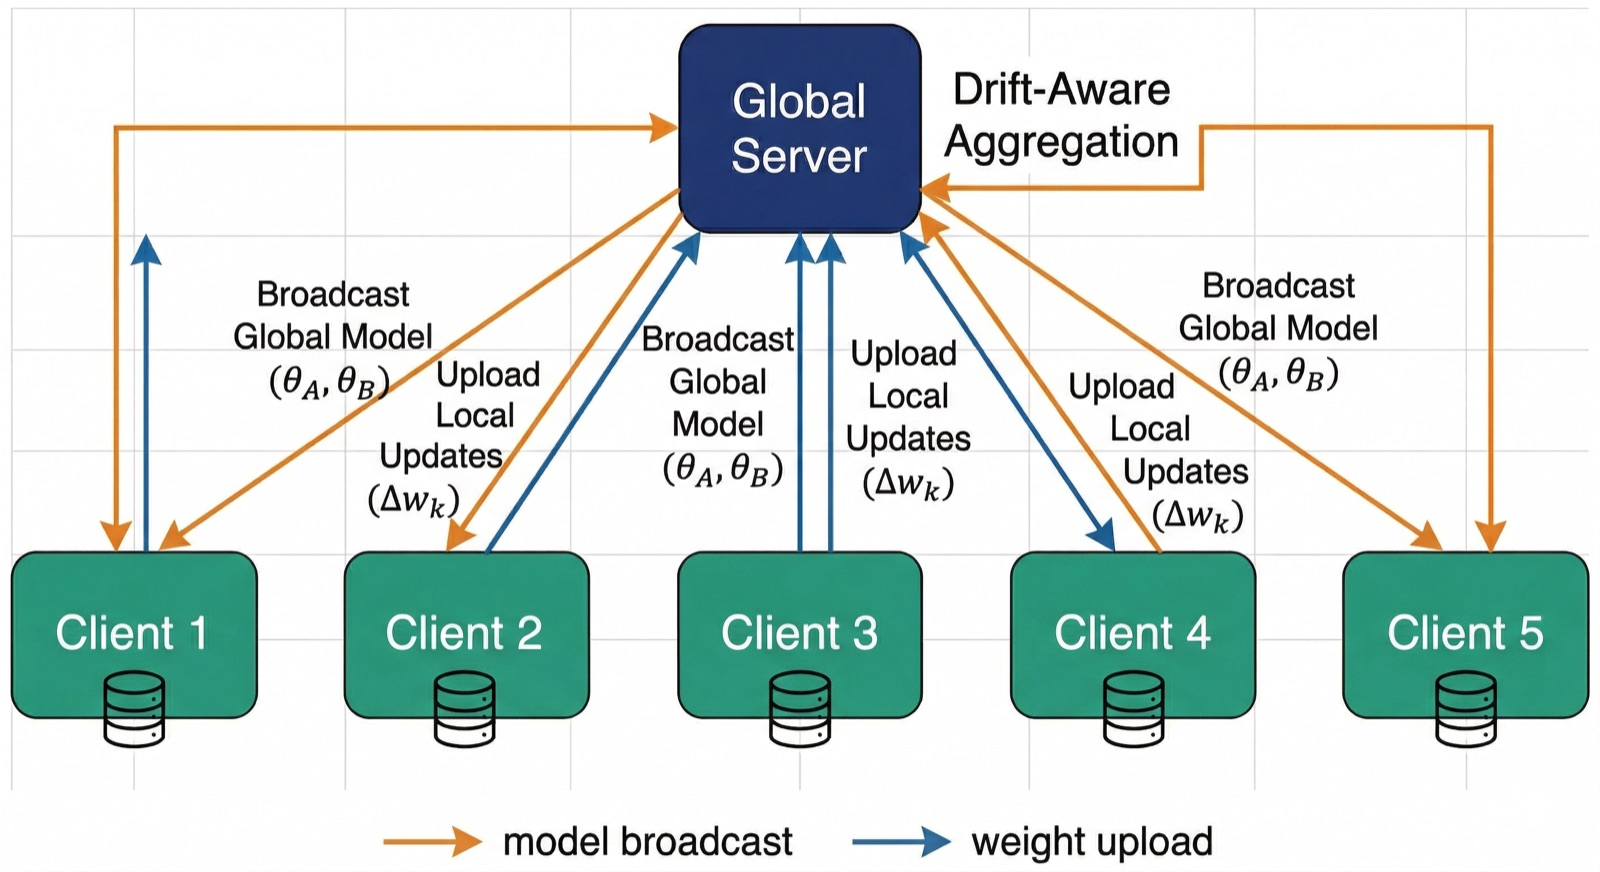
\includegraphics[width=0.82\columnwidth]{images/Intro.jpg}
\caption{Overview of the federated learning setup with 5 clients. Each client trains locally on private data and uploads model updates to the global server. The server aggregates updates via drift-aware inverse-distance weighting and broadcasts the updated global model parameters back to all clients.}
\label{fig:intro_federated}
\end{figure}

\subsection{Existing Solutions and Limitations}

Federated Averaging (FedAvg) is the de facto standard for federated optimization algorithms \cite{McMahan2017}. It averages the models from all clients weighted according to the size of the local dataset for each client. The FedAvg algorithm works well when local data distributions are similar to one another. However, when data is non-IID, the local models begin to drift; this means that the local models will converge toward different optimal points, resulting in a biased or unstable aggregate model \cite{Karimireddy2020,Li2020}.

Different methods have been proposed to address this problem. There are proximal regularization methods that introduce a penalty to any local update that deviates from the global model \cite{Li2020}. Alternatively, there are also methods that use control variates or partial personalization strategies \cite{Karimireddy2020,Collins2021}. However, using these additional methods typically requires the introduction of additional hyperparameters or a modification of the objectives that are normally employed to train local models.

For multimodal federated learning, the majority of approaches consider the model a single set of parameters. That is, all layers of all models are aggregated in the same way, regardless of the role of each layer. This does not take into account that the early feature extractors and the deep semantic layers will behave very differently under any change in distribution. As a result, uniform aggregation produces instability in shared representations and limits the ability of institutions to specialize \cite{Zhu2025}.

In addition to this, many researchers and practitioners tend to focus on global metrics such as overall accuracy or AUC. For clinical applications, however, global performance alone is not adequate. For example, a model that performs well on average, but fails at one institution, will create inequities and diminish trust \cite{Darzi2024,Li2021}.

\subsection{Research Gap}

There are still critical gaps that exist in federated medical learning despite past progress.

Sensitivity to layer-wise distributional heterogeneity: Compared to the earlier feature extraction layers, the performance of later deep Transformer model layers is more adversely impacted by distributional heterogeneity. Research on federated Vision Transformers indicates that if the multi-head attention remains misaligned across multiple client devices, the performance of the other clients will suffer due to feature collapse \cite{Darzi2024}. Studies evaluating partially personalized models show that uniformly aggregating shared model parameters negatively impacts the device drift experienced by clients \cite{Zhu2025}. Most current methods uniformly aggregate all shared model parameters while failing to take into account the different functional behaviours exhibited by the various layers of the model.

Multimodal personalization: Structured clinical metadata frequently varies greatly across hospitals (e.g., age, gender and body structure) \cite{Nunnari2020}. When using multimodal federated models, if the shared visual and the personalized components of the metadata are not kept separate from each other, the divergence of each will increase, thereby decreasing stability \cite{Zhu2025}. Most current methods do not appropriately enforce a separation between these two components.

Client-level stability under severe non-IID conditions: Individual clients may experience substantial drops in performance under conditions of severe non-IID distributional heterogeneity, even though the global metric remains satisfactory. Recent research on federated Vision Transformers shows that there is a critical requirement for the robustness of the worst client in order to stabilise client performance \cite{Darzi2024,Zhao2025}. The majority of current methods are primarily directed toward achieving a global objective and do not provide a mechanism for optimising worst-case client performance.

Moreover, many of the technical methods used to stabilise client performance impose extensive computation costs on client devices, while it is very important that efficiency be considered when developing practical applications for resource-limited environments \cite{Wu2024}. There is therefore a clear need for a federated method that stabilizes critical representation layers and improves fairness without complex local regularization.

\subsection{Objectives}

The objective of this research is to develop a federated multimodal skin lesion classification framework that incorporates the concept of data structure upon which it is designed. Additionally, the framework will be designed with the express intent of being resilient to the different forms of data distribution (heterogeneous data distributions).

This research will accomplish its objectives by developing:


\begin{itemize}
    \item A method to decompose parameters that separates global visual representations from client-specific multimodal heads.
    \item An aggregation mechanism to address client divergence using available data from clients on the server-side.
    \item An examination of how the model behaves under IID versus non-IID conditions, as simulated using a Dirichlet distribution.
    \item A comparison between the performance of federated learning versus the maximum achievable performance of centralized learning.
    \item An evaluation of fairness in terms of worst-case client accuracy and the inter-client standard deviation of accuracy for all models.
\end{itemize}

\subsection{Major Contributions}

This paper makes four algorithmic and design contributions and three empirical ones. We separate them because two of the strongest results below are findings about evaluation rather than new machinery. The algorithmic contributions are:

\begin{itemize}
    \item \textbf{Structure-Aware Parameter Decomposition:} Model parameters are decomposed in a manner that separates early backbone layers, deep Transformer layers, and client-specific multimodal heads. With this design, the server can selectively aggregate contributions from clients based on the functional role each parameter group plays.

    \item \textbf{Drift-Aware Inverse-Distance Aggregation:} The aggregation mechanism designed for the server-side reduces the overall contribution of outlier clients based on how far they have drifted from prior models. No changes to local training objectives need to be made, nor are any additional regularization hyperparameters required.




    \item \textbf{Fairness at the Client Level:} The results indicated that worst-performing clients benefited from drift-aware aggregation versus decomposition alone, while the overall variance between clients was significantly lower.

    \item \textbf{Practical Viability:} The computational overhead incurred by \sadrift{} versus FedAvg was very minor; therefore, it can be practically implemented to facilitate medical-based deployment at multiple institutions.

\end{itemize}

The empirical contributions are:

\begin{itemize}
    \item \textbf{Class Abandonment Under Severe Skew:} We show that standard FedAvg can drive recall on a clinically critical class to exactly zero under severe label skew while retaining competitive aggregate accuracy, and that this failure is invisible to overall and balanced accuracy alike. This argues for reporting per-class coverage as a first-class metric in federated medical imaging.
    \item \textbf{Component Decomposition Ablation:} A three-way comparison at $\alpha = 0.1$---no decomposition, decomposition only, and full \sadrift{}---separates the roles of the two mechanisms. The parameter decomposition is responsible for preserving class coverage, while drift-aware weighting is responsible for recovering utility and reducing client dispersion. Neither component is redundant and neither is sufficient alone.
    \item \textbf{Proof-of-Concept Heterogeneity Study:} The performance of \sadrift{} was evaluated from near-IID through severely heterogeneous data distributions using three Dirichlet concentration parameters ($\alpha \in \{0.1, 0.5, 1.0\}$) and two client counts ($K \in \{3, 5\}$) on the ISIC 2019 dataset, with the severe setting additionally validated on a held-out test split. This constitutes an initial empirical characterization; evaluation at larger client counts is left to future work.


\end{itemize}

\section{Literature Survey}
\subsection{Survey of Existing Methods}
\subsubsection{Transformer-Based Vision Models}
Automated classification of skin lesions has moved from CNN methods to Vision Transformers (ViTs) that leverage self-attention to capture long-range dependencies. ViTs outperform traditional CNN methods, especially when the class distribution is imbalanced \cite{Aguirre2024}. Hybrid models are now the most common state-of-the-art methods due to their ability to combine local and global features. Strong attention-based fusion models combining ConvNeXt and ViT have produced state-of-the-art performance on ISIC datasets \cite{Naeem2025}. Multi-stream architectures using transformers can extract multi-scale patterns in dermatology \cite{Alshdaifat2025}. Other approaches include segmentation/classification fusion \cite{HyperFusionNet2025}, ensemble models that take into account metadata \cite{HasanRifat2024}, and transformer ensembles that utilize uncertainty as part of the fusion process \cite{Zoravar2024}.
\subsubsection{Skin Lesion Datasets and Benchmarking}
ISIC 2019 and ISIC 2020 are recognized as the standard benchmarks for skin lesion classification because they provide a number of challenges, such as class imbalance, heterogeneous quality of the images, and the presence of out-of-distribution samples. The top-performing methods typically utilize multi-resolution architectures, extensive augmentation of the training data, and a loss function that balances the classes \cite{Gessert2020}. Additionally, incorporating structured demographic information into the classification process increases diagnostic performance \cite{Nunnari2020}. However, the presence of artifacts such as occlusions caused by hair or measurement markers makes the preprocessing of the data more complex \cite{Wegley2026}. Finally, the presence of demographic imbalances in the datasets implies that there may be issues with classification fairness or generalizability \cite{SkinDiversity2024}.
\subsubsection{Federated Learning in Medical Imaging}
Federated Learning (FL) allows for private, cooperative training that meets the GDPR and HIPAA laws \cite{Guan2024}. Initial implementations used small convolutional neural networks that ran Federated Averaging to learn from multiple institutions \cite{Subramanian2025}. By utilizing communication-efficient techniques, such as asynchronous updates at the layer level, the amount of bandwidth required was significantly reduced \cite{Yaqoob2023}. However, there are still issues with data being non-independent and identically distributed (non-IID) between the various participating institutions, and class imbalance exists as well. Dynamic Adaptive Focal Loss is one method of correcting for class imbalance, but it also increases the computational burden and sensitivity to hyperparameters involved \cite{Zhao2025}.
\subsubsection{Federated Vision Transformers}
Federated settings with Vision Transformers create additional computation and communication challenges compared to Federated Convolutional Neural Networks, due in part to their architecture. Strategies to increase efficiency include masking patches during training \cite{Wu2024} and pruning layers in the ViT architecture \cite{Paxton2024}. In addition to being adversely affected by non-IID data, feature collapse is also an issue with Federated ViT learning. Some alignment-based methods have been developed to ensure consistent representation of local and global attention \cite{Darzi2024}. Lastly, personalization and continual learning strategies are being investigated to improve the adaptability of the Federated ViT learning process \cite{Zuo2024,Yao2024}.
\subsubsection{Explainability, Security and System Architectures}
Concerns regarding the robustness, privacy, and interpretability of federated systems have been documented. One way to improve the stability of representations in a federated system is through self-ensembling \cite{Almalik2022}. Techniques for mitigating the effects of adversarial attacks include diffusion-based defenses \cite{Imam2023}. Privacy-preserving techniques, such as random projection, have been suggested as a way to improve communication security between federated clients and providers \cite{Narimani2024}. In multimodal systems, partial personalization leads to better adaptation at the local client; however, it increases the potential for client drift, and thus optimization-based corrections are required \cite{Zhu2025}.
\subsection{Comparative Analysis}
Standalone architectures have consistently been outperformed by hybrid CNN–Transformer models when used in centralized cases \cite{Naeem2025,Alshdaifat2025}. In federated environments, a trade-off exists between model consistency and computational resource efficiency. Alignment-based approaches result in improved model stability but come with a very high overhead cost. Efficiency-based methods reduce the amount of computational resources required to run the models, but at the expense of representational fidelity.
\subsection{Relation to Personalized and Drift-Corrected Federated Learning}
\label{sec:positioning}

\sadrift{} combines partial parameter personalization with adaptive server-side aggregation. Neither ingredient is new, and we do not claim otherwise. What follows states precisely what is and is not different from the established alternatives, since the combination is the contribution rather than either component.

\textbf{Partial personalization.} FedPer~\cite{Collins2021} and FedRep~\cite{Collins2021} keep a classification head local and share a representation; FedBABU trains the body with the head frozen and personalizes only at the end; FedBN keeps normalisation statistics local. \sadrift{}'s Group~C is the same idea as FedPer's private head, extended to a multimodal head that also carries the metadata branch. The difference from all four is not the existence of a private head but that the \emph{shared} portion is itself split, with early and deep layers aggregated by different rules---FedPer, FedRep, FedBABU and FedBN all apply one aggregation rule to everything they share.

\textbf{Drift correction.} FedProx adds a proximal term to the local objective; SCAFFOLD maintains per-client control variates that correct the local update direction; FedDyn adds a dynamic regulariser; FedNova normalises for unequal local step counts. All four act on the client. \sadrift{} leaves the local objective and optimiser untouched and acts only on the aggregate. This is the practical distinction we emphasise: no additional hyperparameter is tuned, no auxiliary state of model size is stored per client, and clients require no modification. It is also a weaker form of correction, since the server cannot see the trajectory that produced a client's parameters.

\textbf{What is genuinely new here is narrow.} Applying depth-dependent aggregation rules within a Vision Transformer backbone---plain averaging for early layers, drift-weighted averaging for deep layers---together with a private multimodal head, is a configuration we have not found in the prior work. Our empirical finding about class abandonment is independent of that configuration and would apply to any comparison of aggregation schemes.

\textbf{We have not measured against these methods.} None of FedProx, SCAFFOLD, FedBN, FedRep, FedPer, FedBABU, FedNova or FedDyn was re-implemented under our conditions. Our comparisons are to FedAvg, to the decomposition without drift weighting, and to a no-decomposition variant. We therefore cannot state whether the gains reported here would persist against a strong personalized baseline such as FedRep or FedBN, and we do not claim they would. Section~\ref{sec:threeway} isolates the contribution of each of our own components, which is a different and narrower question than superiority over the personalized federated learning literature. Establishing the latter requires the comparison set above and is the primary item of future work.

\subsection{Limitations in Prior Work}
\begin{enumerate}
\item \textbf{Client Drift in Heterogeneous Settings:} The client drift phenomenon refers to a non-IID data distribution present in heterogeneous settings, which may cause instability in convergence and thus reduce global performance \cite{Zhu2025}.
\item \textbf{Destructive Efficiency Techniques:} Aggressive masking and/or pruning can cause disruption of the representation of hierarchical aspects of transformer models \cite{Wu2024}.

\item \textbf{Complex Loss Engineering:} Because of the introduction of adaptive loss functions, the number of hyperparameters has increased, which adds computational overhead in the form of extra computation \cite{Zhao2025}.

\item \textbf{Feature Collapse under Uniform Aggregation:} Due to the standard aggregation process used in federated learning, the diversity of hierarchical features will not be maintained under uniform aggregation \cite{Darzi2024}.

\subsection{Mathematical and Computational Complexity Analysis}
\subsubsection{Formal Computational Complexity}
The use of large Vision Transformer models in federated learning can require a lot of extra computational resources due to their size, especially when the device is an edge device \cite{Wu2024}. For a model with parameter size $|w|$, local training complexity scales as:
\begin{equation}
\mathcal{O}(E \cdot |w|),
\end{equation}
where $E$ is the number of local epochs. Optimization-based approaches further increase this cost due to additional penalty terms and dual-variable updates. Alignment-based methods also introduce overhead proportional to the attention dimensions, typically $\mathcal{O}(h d^2)$ \cite{Darzi2024}.
\subsubsection{Communication Efficiency Considerations}
Standard federated learning models transmit all the parameters of the model for every round of training, which results in a very high communication cost. Therefore, due to the full parameter transmission of large transformer models, communication costs are high as well. Compression and selective updates can help reduce bandwidth usage, but typically reduce the performance and representational capacity of the model.

\end{enumerate}
\begin{table*}[h]
\centering
\small
\caption{Comparison of hybrid and federated skin lesion classification methods and their limitations.}
\label{tab:literature_comparison}
\begin{tabular}{@{}p{0.14\linewidth} p{0.16\linewidth} p{0.32\linewidth} p{0.30\linewidth}@{}}
\toprule
\textbf{Author(s)} & \textbf{Model / Framework} & \textbf{Key Innovation} & \textbf{Limitation} \\
\midrule
Naeem et al.~\cite{Naeem2025}
& MedFusionNet
& Attention-based fusion of ConvNeXt and ViT
& Centralized architecture; does not address federated privacy constraints \\[4pt]
Gessert et al.~\cite{Gessert2020}
& Multi-Resolution EfficientNets
& Ensemble with metadata fusion (ISIC 2019 winner)
& Requires centralized metadata aggregation \\[4pt]
Zhao et al.~\cite{Zhao2025}
& FL with DAFL
& Dynamic loss adaptation for class imbalance
& Hyperparameter-sensitive; increased computational overhead \\[4pt]
Wu et al.~\cite{Wu2024}
& EFTViT
& Patch masking for efficient federated ViT training
& Disrupts spatial and hierarchical representations \\[4pt]
Darzi et al.~\cite{Darzi2024}
& FedMHA
& Attention alignment to mitigate feature collapse
& Computationally expensive regularization \\[4pt]
Zhu et al.~\cite{Zhu2025}
& FedAPM
& ADMM-based personalization to reduce drift
& High optimization complexity \\[4pt]
Yaqoob et al.~\cite{Yaqoob2023}
& Async-FL-CNN
& Asynchronous updates for communication efficiency
& Limited to CNNs \\[4pt]
Paxton et al.~\cite{Paxton2024}
& Skewness-Guided Pruning
& Model compression for edge deployment
& Reduces model capacity \\[4pt]
Narimani et al.~\cite{Narimani2024}
& FedRP
& Random projection for privacy preservation
& Does not address data heterogeneity \\
\bottomrule
\end{tabular}
\end{table*}

\section{Methodology}

\subsection{Methodology Overview}

This part discusses how to create the \sadrift{} training workflow step by step.
\begin{enumerate}
\item Set up the federated multimodal problem and notation.
\item Create heterogeneous client datasets with Dirichlet partitions.
\item Create a centralized upper bound baseline.
\item Decompose the parameters of the model into groups that preserve the structure of the data.
\item Train the model using local computation and then aggregate the results globally using drift-aware weighting.
\end{enumerate}

Figure~\ref{fig:framework} shows the structure-aware federated aggregation architecture.

\subsection{Problem Setup and System View}

The goal of \sadrift{} is to train a shared model across $K$ clients without exchanging any raw data between clients. Each client holds their own local dataset:

\begin{equation}
\label{eq:local_dataset}
\mathcal{D}_k = \{(x_i^k, m_i^k, y_i^k)\}_{i=1}^{n_k}
\end{equation}

where $x_i^k$ represents the $i$-th dermoscopic image, $m_i^k$ represents the clinical metadata associated with that image in structured format, and $y_i^k \in \{1,\ldots,C\}$ represents the label or class of the lesion in the image. The total number of samples across $K$ clients is $N = \sum_{k=1}^{K} n_k$.

The common goal is to develop a multimodal classifier defined as:
\begin{equation}
\label{eq:classifier}
f_\theta : (x,m) \mapsto \hat{y}
\end{equation}

where $\theta$ is the parameter vector of the model and $\hat{y}$ is the predicted classification label.

\begin{figure}[t]
\centering
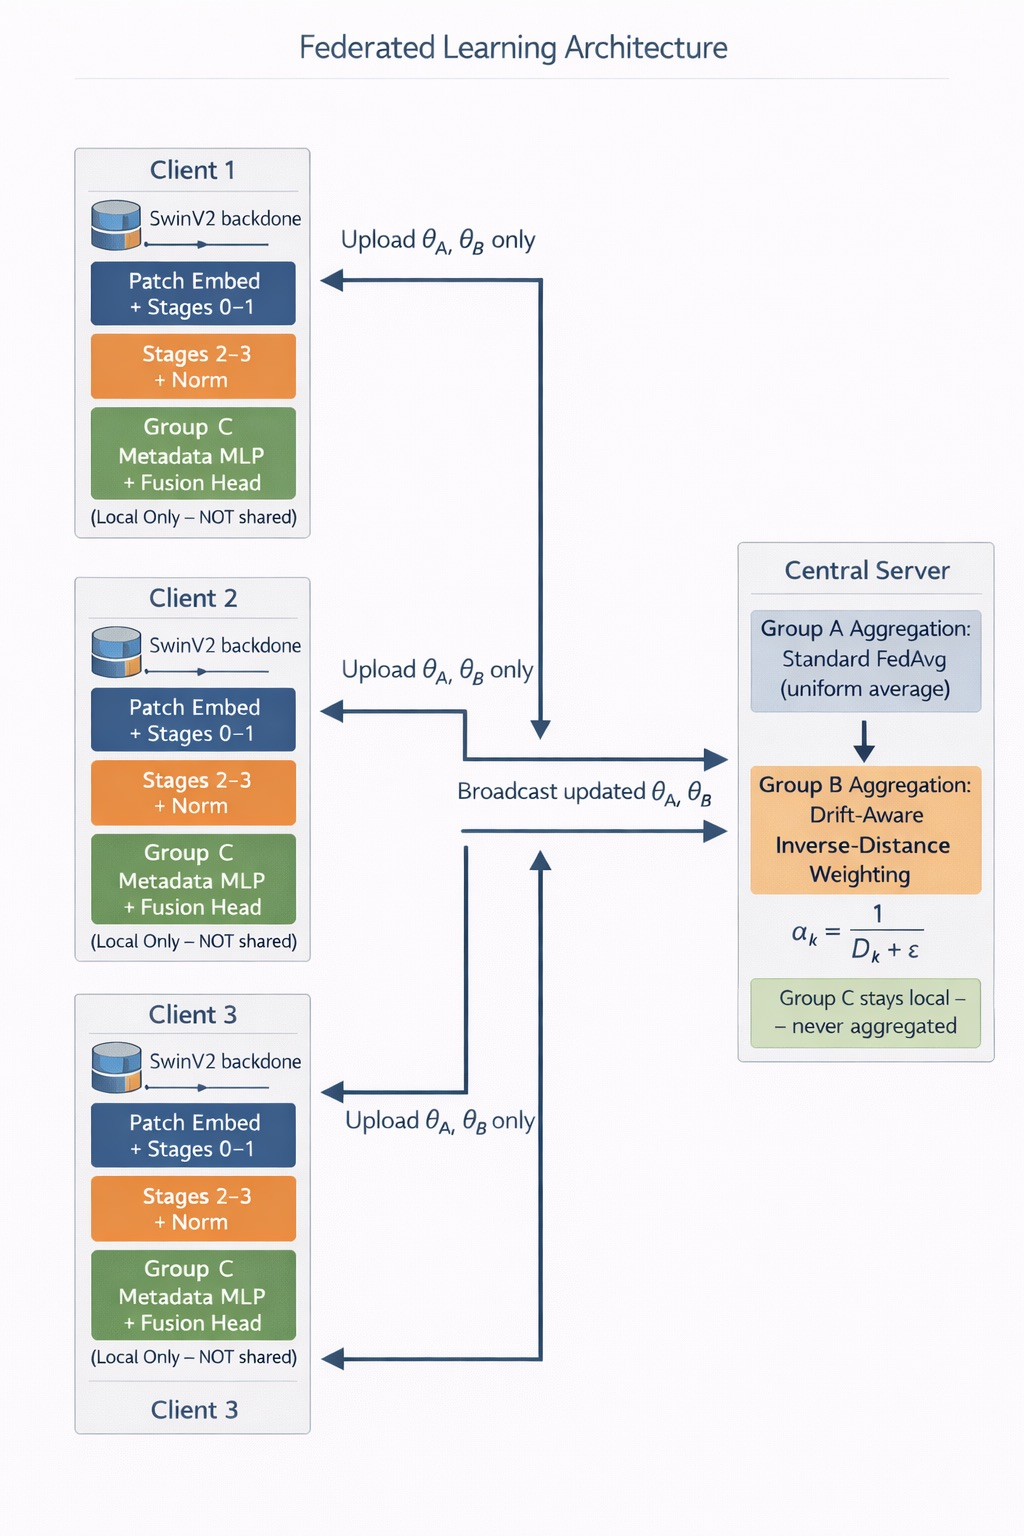
\includegraphics[width=0.90\columnwidth]{images/federated learning.jpg}
\caption{Structure-aware federated aggregation architecture.}
\label{fig:framework}
\end{figure}

\subsection{Step 1: Dirichlet Non-IID Data Partitioning}

Each client's data is sampled from a Dirichlet prior to simulate the true heterogeneity that exists across multiple clients:

\begin{equation}
\label{eq:dirichlet}
\pi_k \sim \text{Dir}(\alpha)
\end{equation}

where $\pi_k \in \Delta^{C-1}$ is the class-proportion vector for client $k$ and $\alpha > 0$ is the concentration parameter. A smaller value for $\alpha$ gives more skewed class distributions across clients, and a larger value provides more uniform ones. We evaluate $\alpha \in \{1.0, 0.5, 0.1\}$. At $\alpha = 0.1$ the draw is degenerate in a way that matters for the results: with $K = 5$ one client receives no samples whatsoever for four of the eight classes, two more are missing three and two classes respectively, and that same largest client receives 53\% of the federation's data. A partition is accepted only if every client holds at least two classes and at least 100 samples; this admits the $\alpha = 0.1$ draw used here, whose per-client class counts are listed in Section~\ref{sec:severe_setting}.

The fraction of class-$c$ samples at client $k$ is:

\begin{equation}
\label{eq:class_proportion}
p_{kc} = \frac{n_{kc}}{n_k}
\end{equation}

The variance of these proportions across multiple clients is given by:

\begin{equation}
\label{eq:dirichlet_variance}
\text{Var}(p_{kc}) =
\frac{\alpha (C\alpha - \alpha)}
{(C\alpha)^2 (C\alpha + 1)}
\end{equation}

As $\alpha \to 0$, the variance increases, which represents the degree to which distributions across multiple clients will diverge based on the value assigned to the alpha parameter, leading to client gradients diverging:

\begin{equation}
\label{eq:gradient_divergence}
\nabla F_k(\theta) \neq \nabla F_j(\theta), \quad k \neq j
\end{equation}

This gradient misalignment is the core challenge in the federated learning scenario.

\subsection{Step 2: Centralized Training Baseline}

The data of all clients must be pooled together in order to create a reference upper bound:

\begin{equation}
\label{eq:pooled_data}
\mathcal{D} = \bigcup_{k=1}^{K} \mathcal{D}_k
\end{equation}

Empirical risk minimization (ERM) is used as the central target:

\begin{equation}
\label{eq:centralized_objective}
F(\theta)
=
\frac{1}{N}
\sum_{k=1}^{K}
\sum_{i=1}^{n_k}
\ell(f_\theta(x_i^k,m_i^k), y_i^k)
\end{equation}

where $\ell(\cdot,\cdot)$ is the per-sample cross-entropy loss. Written schematically as gradient descent, the update dynamics are:

\begin{equation}
\label{eq:centralized_update}
\theta^{t+1} = \theta^t - \eta \nabla F(\theta^t)
\end{equation}

All reported experiments use AdamW rather than plain gradient descent; Equation~\eqref{eq:centralized_update} is written in this form only to define the objective being descended.

where $\nabla F(\theta^t) = \frac{1}{N}\sum_{k}\sum_{i} \nabla \ell(f_\theta(x_i^k,m_i^k), y_i^k)$.

The model is trained for $E$ epochs using AdamW with a cosine learning rate schedule:

\begin{equation}
\label{eq:centralized_admw}
\theta^{E} = \text{AdamW}(\theta^0, \mathcal{D})
\end{equation}

In a centralized context, there is no client drift and therefore no communication overhead. As such, the performance of this model acts as a reference upper bound for all subsequent federated experiments.

\begin{figure}[htbp]
\centering
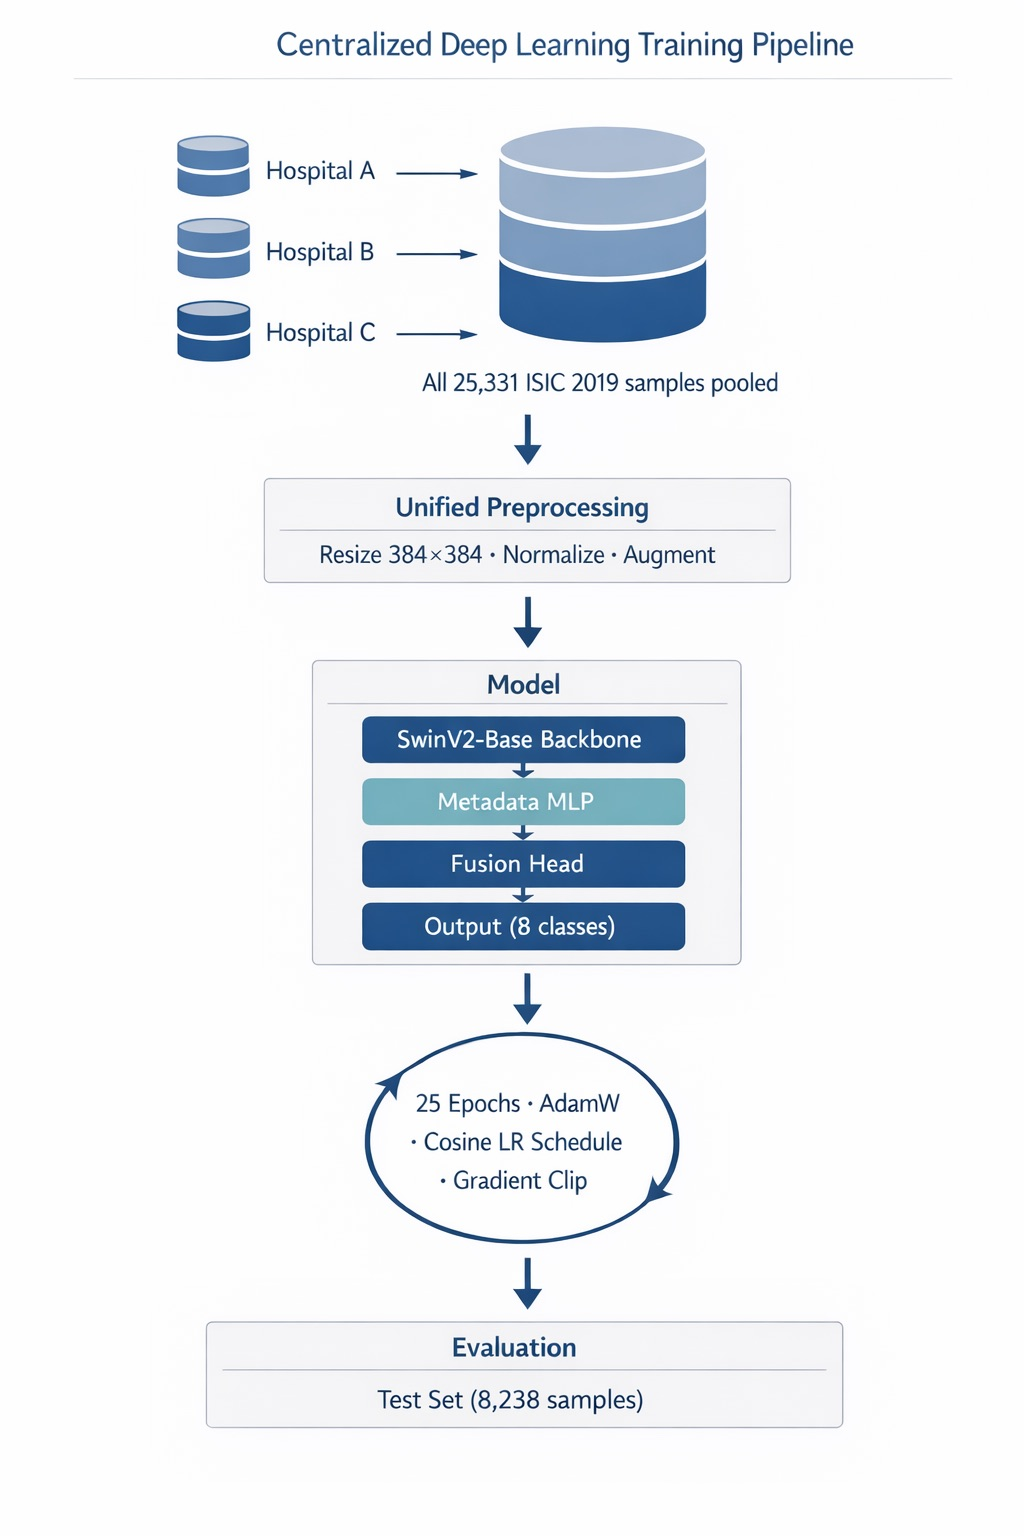
\includegraphics[width=0.45\textwidth]{images/centralized.jpg}
\caption{Centralized training pipeline using pooled multimodal data.}
\label{fig:centralized_flow}
\end{figure}

\subsection{Step 3: Federated Optimization Objective}

In federated learning, the global goal is the weighted average of all of the local objectives:

\begin{equation}
\label{eq:fed_objective}
F(\theta) = \sum_{k=1}^{K} \frac{n_k}{N} F_k(\theta)
\end{equation}

where $F_k(\theta)$ is the risk value for each client and is defined as:

\begin{equation}
\label{eq:local_risk}
F_k(\theta) = \frac{1}{n_k} \sum_{i=1}^{n_k} \ell(f_\theta(x_i^k,m_i^k), y_i^k)
\end{equation}

The server averages the gradients of all clients to generate the global gradient:

\begin{equation}
\label{eq:fed_gradient}
\nabla F(\theta) = \sum_{k=1}^{K} \frac{n_k}{N} \nabla F_k(\theta)
\end{equation}

When there are differences between the distributions of clients, this approximation becomes biased due to client drift.

\subsection{Step 4: Structure-Aware Parameter Decomposition}

To mitigate drift, \sadrift{} assigns each parameter to one of three functional groups:

\begin{equation}
\label{eq:param_decomp}
\theta = \{\theta_A, \theta_B, \theta_{C,k}\}
\end{equation}

\begin{itemize}
\item \textbf{Group A} ($\theta_A$) contains the patch embedding and early SwinV2 stages (0--1). These capture low-level visual features that generalize across institutions, and are aggregated by standard FedAvg.
\item \textbf{Group B} ($\theta_B$) contains the late SwinV2 stages (2--3) and layer normalization. These encode high-level semantics that are most sensitive to distribution shifts, and are aggregated with drift-aware weighting.
\item \textbf{Group C} ($\theta_{C,k}$) contains the client-specific metadata MLP and fusion head. These are never transmitted to the server.
\end{itemize}

The predicted output for sample $i$ at client $k$ is:

\begin{equation}
\label{eq:prediction}
\hat{y}_i^k = g_{\theta_{C,k}}\!\left(h_{\theta_A,\theta_B}(x_i^k),\, m_i^k\right)
\end{equation}

where $h_{\theta_A,\theta_B}$ is the shared SwinV2 backbone and $g_{\theta_{C,k}}$ is the local fusion head. As long as Group C is maintained locally, this enables the models to be personalized for each institution while still securing the confidentiality of the metadata.

\subsection{Step 5: Local Client Optimization}

Clients apply local training of the models via AdamW, where the backbone is trained at a $0.1\eta$ learning rate and the metadata MLP and fusion head use the $\eta$ learning rate. In addition, a cosine schedule with linear warmup is used for all parameters in both groups. The update rule is:

\begin{equation}
\label{eq:local_update}
\theta_k^{t+1} = \text{AdamW}(\theta^t, \nabla F_k(\theta^t), \eta)
\end{equation}

For the structured (grouped) parameters:

\begin{equation}
\label{eq:groupA_update}
\theta_{A,k}^{t+1} = \text{AdamW}\!\left(\theta_A^t,\, \nabla_{\theta_A} F_k,\, 0.1\eta\right)
\end{equation}

\begin{equation}
\label{eq:groupB_update}
\theta_{B,k}^{t+1} = \text{AdamW}\!\left(\theta_B^t,\, \nabla_{\theta_B} F_k,\, 0.1\eta\right)
\end{equation}

where $\nabla_{\theta_A} F_k$ and $\nabla_{\theta_B} F_k$ are the partial gradients of local risk at the clients. These per-client updates diverge across institutions under non-IID conditions. It is for this reason that drift-aware aggregation is needed, as described in Section~\ref{sec:drift_agg}.

\subsection{Step 6: Server-Side Drift-Aware Aggregation}
\label{sec:drift_agg}

Once local training is complete, the parameters for Groups A and B are uploaded to the server, where standard FedAvg is used to aggregate Group A and drift-aware weighting is used to de-emphasise updates from clients in Group B that deviate from the consensus. Furthermore, there are no changes to the local training objectives or the addition of hyperparameters.

\subsubsection{Distance Computation}

The server computes the mean across clients for every parameter tensor $l \in \theta_B$:

\begin{equation}
\label{eq:consensus_mean}
\bar{w}_l = \frac{1}{K} \sum_{k=1}^{K} w_{k,l}
\end{equation}

where $w_{k,l}$ is the tensor uploaded by client $k$. To calculate the client drift from the mean across clients, the Euclidean distance between the client update and the mean is computed:

\begin{equation}
\label{eq:drift_distance}
D_{k,l} = \| w_{k,l} - \bar{w}_l \|_2
\end{equation}

The $L_2$ norm is used here because model parameters exist within a Euclidean space. It is computationally efficient and gives an accurate measurement of how far every client update deviates from the mean across clients.

\subsubsection{Inverse-Distance Weighting}

Each client receives an unnormalised weight calculated using its drift:

\begin{equation}
\label{eq:inv_weight}
\alpha_{k,l} = \frac{1}{D_{k,l} + \epsilon}
\end{equation}

where $\epsilon = 10^{-6}$ avoids division by zero. This therefore gives more weight to clients that are near consensus and proportionally less weight to clients that are far from consensus.

The inverse approach is preferred to an exponential, e.g., $\exp(-\beta D_{k,l})$, as it has the following advantages:
\begin{itemize}
\item It does not require any additional sensitivity parameter $\beta$.
\item It will not cause a complete collapse of weights toward 0 in the case of large values of $D_{k,l}$.
\item A smooth heavy-tailed profile of decay in the weights is achieved.
\end{itemize}

Weights are normalized so that they sum to 1:

\begin{equation}
\label{eq:norm_weight}
\hat{\alpha}_{k,l} = \frac{\alpha_{k,l}}{\sum_{j=1}^{K} \alpha_{j,l}}
\end{equation}

The total combined Group B tensor is:

\begin{equation}
\label{eq:groupB_agg}
\theta_{B,l}^{t+1} = \sum_{k=1}^{K} \hat{\alpha}_{k,l} \cdot w_{k,l}
\end{equation}

\subsubsection{Convergence Analysis (Informal Argument)}

\noindent\textbf{Assumptions.}
The following informal argument assumes that each local objective $F_k$ is $L$-smooth (i.e., $\|\nabla F_k(\mathbf{u}) - \nabla F_k(\mathbf{v})\| \le L\|\mathbf{u}-\mathbf{v}\|$ for all $\mathbf{u},\mathbf{v}$) and that stochastic gradient noise has bounded second moment. This analysis is not a formal convergence proof and does not derive a rate; its purpose is to make precise the intuitive stability benefit of drift-aware attenuation under standard conditions.

Let $\Delta_k^t = \mathbf{w}_k^t - \mathbf{w}^t$ denote the local update of client $k$ at round $t$. Standard FedAvg combines updates as:

\begin{equation}
\label{eq:fedavg_agg}
\mathbf{w}^{t+1} = \mathbf{w}^t + \sum_{k=1}^{K} p_k \Delta_k^t
\end{equation}

where $p_k = n_k / N$. In \sadrift{}, each Group~B update is attenuated by a scalar factor $\gamma_k^t \in (0,1]$ derived from the inverse-distance weight $\hat{\alpha}_{k,l}$, giving an effective update $\tilde{\Delta}_k^t = \gamma_k^t \Delta_k^t$:

\begin{equation}
\label{eq:sadrift_agg}
\mathbf{w}^{t+1} = \mathbf{w}^t + \sum_{k=1}^{K} p_k \tilde{\Delta}_k^t
\end{equation}

Since $\gamma_k^t \le 1$ for all $k$, the $\ell_2$ norm of the aggregate step is bounded:

\begin{equation}
\label{eq:stability_bound}
\left\|\sum_{k=1}^K p_k \tilde{\Delta}_k^t\right\|_2
\;\le\;
\left\|\sum_{k=1}^K p_k \Delta_k^t\right\|_2
\end{equation}

Clients with the largest drift (large $D_{k,l}$, hence small $\gamma_k^t$) receive the smallest weight, pulling the aggregate toward the cross-client consensus.

We must be explicit about the gap between this expression and Algorithm~\ref{alg:federated}. Equation~\eqref{eq:stability_bound} holds for an aggregate of the form $\sum_k p_k \gamma_k \Delta_k$ with size weights $p_k = n_k/N$ retained and $\gamma_k \le 1$ applied on top. The implemented Group~B rule does not do this: it \emph{replaces} the size weights with normalised inverse-distance weights $\hat{\alpha}_{k,l}$ that sum to one, so a client close to consensus can receive a weight substantially larger than its $p_k$. The contraction in Equation~\eqref{eq:stability_bound} therefore does not follow for the algorithm as implemented, and we do not claim it does. A second gap is that the aggregation rules of Equation~\eqref{eq:groupB_agg} and its Group~A counterpart combine parameters $\mathbf{w}_{k,l}$ whereas Equations~\eqref{eq:stability_bound} onward reason about updates $\Delta_k$; these coincide only when every client starts the round from the same point, which holds for Groups~A and~B but not for the personalized Group~C.

What follows below should accordingly be read as motivation for why down-weighting divergent clients is expected to reduce round-to-round oscillation, not as a proof about the deployed procedure. A convergence analysis of normalised inverse-distance aggregation is left to future work.

\subsubsection{Properties and Failure Modes of the Weighting}
\label{sec:weight_analysis}

The weight assigned to client $k$ for parameter tensor $l$ is
$\hat{\alpha}_{k,l} = (D_{k,l}+\epsilon)^{-1} / \sum_j (D_{j,l}+\epsilon)^{-1}$
with $\epsilon = 10^{-6}$. Three properties follow directly and should be stated, since two of them are potential failure modes.

\emph{The scheme can be dominated by a single client.} Writing $D_{\min}$ and $D_{\max}$ for the smallest and largest drift among the $K$ clients,
\begin{equation}
\hat{\alpha}_{\max} \;\le\; \left[1 + (K-1)\frac{D_{\min}+\epsilon}{D_{\max}+\epsilon}\right]^{-1} .
\end{equation}
As $D_{\min} \to 0$ with $\epsilon \ll D_{\max}$, this bound approaches 1: a client whose Group~B parameters coincide with the cross-client mean absorbs essentially the entire aggregate. Because $\bar{\mathbf{w}}_l$ is the unweighted mean, $\sum_k (\mathbf{w}_{k,l} - \bar{\mathbf{w}}_l) = 0$, so $D_{\min}$ cannot vanish unless all clients are identical; but it can become small, and the guard against this is $\epsilon$ alone. We did not observe divergence at any setting tested, including $\alpha{=}0.1$, but we have not characterised the regime in which it would occur, and a bounded or temperature-controlled variant would be the natural remedy.

\emph{Dataset size is discarded, and the resulting bias must be stated.} Unlike FedAvg, the Group~B rule does not weight by $n_k$: a client holding 1,015 samples and one holding 11,339 are treated identically if their drift is equal. This is deliberate, but it changes the objective being optimised and warrants a formal statement.

Federated averaging with $p_k = n_k/N$ is the natural estimator for the pooled empirical risk $F(\mathbf{w}) = \sum_k p_k F_k(\mathbf{w})$, in the sense that the aggregate is an unbiased combination of per-client quantities under that weighting. Replacing $p_k$ with $\hat{\alpha}_{k,l}$ introduces a per-tensor bias
\begin{equation}
\label{eq:agg_bias}
\mathbf{b}_l \;=\; \sum_{k=1}^{K} \left(\hat{\alpha}_{k,l} - p_k\right)\mathbf{w}_{k,l},
\end{equation}
so the aggregate no longer estimates the minimiser of $F$. The magnitude of $\mathbf{b}_l$ is governed by the relationship between drift and dataset size. Where the two are positively associated---large clients producing more stable, near-consensus updates because they hold more data---the reweighting is mild and $\hat{\alpha}_{k,l} \approx p_k$. Where they are negatively associated, the reweighting is large and deliberate.

The $\alpha{=}0.1$ partition is the second case, and it is the case the method is built for. Client~2 holds 52.7\% of the federation's data yet contains only four of the eight classes and no melanoma at all. Under size weighting it determines the aggregate, which is precisely the mechanism producing the zero melanoma recall documented in Section~\ref{sec:threeway}; under inverse-distance weighting its influence is reduced to the extent that its parameters diverge from consensus. The bias in Equation~\eqref{eq:agg_bias} is therefore not incidental---it is the effect being sought. What \sadrift{} optimises is closer to a robust consensus among clients than to the pooled empirical risk, and we should describe it that way rather than as an unbiased federated estimator.

Clinically, this is a defensible trade in a specific circumstance and a poor one in others. A federation containing a large referral centre with a skewed case mix is the motivating case: size weighting hands that centre the model, and the resulting model can fail silently on categories it rarely sees. Where instead the largest site is also the most representative---a plausible and common situation---discarding $n_k$ discards genuine statistical information, and \sadrift{} would be expected to underperform FedAvg. We have not tested that regime. Combined with the concentration bound above, the failure mode to be aware of is a small site whose parameters sit near the mean acquiring influence disproportionate to the evidence it contributes.

An obvious middle ground, $\hat{\alpha}_{k,l} \propto n_k / (D_{k,l}+\epsilon)$, retains size information while still suppressing divergence and would interpolate between the two objectives. We did not evaluate it, and we do not claim the size-free form is optimal.

\emph{On the choice of Euclidean distance.} The reviewer question of whether cosine similarity would serve better admits a partly analytical answer, because the two are not interchangeable in this formulation.

Every client begins the round from the same broadcast point, so $\mathbf{w}_{k,l} = \mathbf{w}_l^t + \Delta_{k,l}$ where $\Delta_{k,l}$ is client $k$'s local update. The cross-client mean is $\bar{\mathbf{w}}_l = \mathbf{w}_l^t + \bar{\Delta}_l$, and therefore
\begin{equation}
\label{eq:drift_equiv}
D_{k,l} = \left\|\mathbf{w}_{k,l} - \bar{\mathbf{w}}_l\right\|_2
        = \left\|\Delta_{k,l} - \bar{\Delta}_l\right\|_2 .
\end{equation}
The shared component cancels exactly. Although the rule is written over parameters, it measures the deviation of each client's \emph{update} from the mean update, which is the quantity of interest.

Cosine similarity has no such property. Since $\|\Delta_{k,l}\| \ll \|\mathbf{w}_l^t\|$ after a single local epoch, $\cos(\mathbf{w}_{k,l}, \bar{\mathbf{w}}_l) = 1 - \mathcal{O}\!\left(\|\Delta\|^2/\|\mathbf{w}^t\|^2\right)$ for every client: the measure is dominated by the shared broadcast point and is near-degenerate. In a numerical check with $\|\Delta\|/\|\mathbf{w}^t\| = 0.04$, representative of one local epoch at our learning rates, the spread of cosine similarities across five clients was $1.4\times10^{-5}$, against a spread of $1.7\times10^{-2}$ for the same quantity computed on the updates. Substituting cosine for Euclidean in Equation~\eqref{eq:drift_equiv} without also re-centring would therefore produce weights that are essentially uniform, and the method would degenerate to plain averaging over Group~B.

The meaningful alternative is cosine similarity on the updates, $\cos(\Delta_{k,l}, \bar{\Delta}_l)$, which discards magnitude and penalises only directional disagreement. This is a substantively different criterion: it would treat a client that moved far along the consensus direction as undrifted, whereas the Euclidean rule penalises it. Which is preferable is an empirical question we have not settled, and we make no claim of optimality for the Euclidean form. We note only that it is not arbitrary---by Equation~\eqref{eq:drift_equiv} it is the natural metric on updates---and that the naive substitution the question suggests would not work. Softmax, exponential and inverse-square weightings likewise remain untested.

Applying the standard descent lemma for $L$-smooth objectives and taking expectations over the stochastic gradient noise:

\begin{equation}
\label{eq:convergence}
\mathbb{E}[F(\mathbf{w}^{t+1})]
\;\le\;
F(\mathbf{w}^t)
- \eta \|\nabla F(\mathbf{w}^t)\|^2
+ \frac{\eta^2 L}{2}\,\mathbb{E}\!\left\|\sum_k p_k \tilde{\Delta}_k^t\right\|^2
\end{equation}

The third term—the noise amplification from the aggregate step—is bounded above by the corresponding FedAvg quantity via Eq.~\eqref{eq:stability_bound}. Intuitively, by suppressing drifted updates, \sadrift{} reduces the round-to-round oscillation of the global model without altering local training objectives. Deriving tight convergence rates under non-IID data and formally bounding gradient divergence under this aggregation scheme are left to future theoretical analysis.

\subsection{Step 7: End-to-End Federated Training Process}

Algorithm~\ref{alg:centralized} shows the centralized baseline. Algorithm~\ref{alg:federated} shows the full \sadrift{} federated procedure across $T$ communication rounds.

% ---- Algorithm 1: Centralized Training -------------------------------- %
\begin{algorithm}[t]
\caption{Centralized Training Baseline}
\label{alg:centralized}
\begin{algorithmic}[1]
\REQUIRE Dataset $\mathcal{D} = \bigcup_{k=1}^{K} \mathcal{D}_k$, pretrained backbone weights $\theta_A^0, \theta_B^0$, total epochs $E$, learning rate $\eta$
\ENSURE Trained model parameters $\theta^E$
\STATE Initialize model: $\theta^0 \leftarrow \{\theta_A^0,\, \theta_B^0,\, \theta_C^0\}$
\FOR{epoch $e = 1$ to $E$}
    \FOR{each mini-batch $(x_i, m_i, y_i) \in \mathcal{D}$}
        \STATE Compute logits: $\hat{y}_i = f_\theta(x_i, m_i)$
        \STATE Compute class-weighted CE loss with label smoothing:
               \[ \mathcal{L} = \mathcal{L}_{CE}^{\text{weighted}}(\hat{y}_i,\, y_i) \]
        \STATE Update via AdamW with cosine LR schedule:
               \[ \theta \leftarrow \theta - \eta\,\nabla_\theta\,\mathcal{L} \]
    \ENDFOR
    \STATE Evaluate on test set; record Balanced Accuracy, F1, ROC-AUC
\ENDFOR
\RETURN $\theta^E$
\end{algorithmic}
\end{algorithm}

% ---- Algorithm 2: FedSA-Drift Federated Training ---------------------- %
\begin{algorithm}[t]
\caption{\sadrift{}: Structure-Aware Drift-Regularized Federated Training}
\label{alg:federated}
\begin{algorithmic}[1]
\REQUIRE $K$ clients with local datasets $\{\mathcal{D}_k\}_{k=1}^K$, rounds $T$, local epochs $E$, learning rate $\eta$, $\epsilon = 10^{-6}$
\ENSURE Global shared parameters $\theta_A^T,\, \theta_B^T$; local parameters $\{\theta_{C,k}^T\}$
\STATE \textbf{Server:} Initialize $\theta_A^0,\, \theta_B^0$ from pretrained SwinV2-Base
\STATE Each client $k$ initializes local head $\theta_{C,k}^0$ independently
\FOR{round $t = 1$ to $T$}
    \STATE \textbf{Server} broadcasts $\theta_A^t,\, \theta_B^t$ to all $K$ clients
    \FOR{each client $k = 1$ to $K$ \textbf{(in parallel)}}
        \STATE Load received backbone: $\theta_{A,k} \leftarrow \theta_A^t$,\; $\theta_{B,k} \leftarrow \theta_B^t$
        \FOR{local epoch $e = 1$ to $E$}
            \FOR{each mini-batch $(x_i^k, m_i^k, y_i^k) \in \mathcal{D}_k$}
                \STATE $\hat{y}_i^k = g_{\theta_{C,k}}\!\left(h_{\theta_{A,k},\theta_{B,k}}(x_i^k),\, m_i^k\right)$
                \STATE $\mathcal{L}_k = \mathcal{L}_{CE}^{\text{weighted}}(\hat{y}_i^k,\, y_i^k)$
                \STATE Update all local params via AdamW (diff.\ LR):
                       $\theta_{A,k},\, \theta_{B,k},\, \theta_{C,k} \leftarrow \text{AdamW}(\mathcal{L}_k,\,\eta)$
            \ENDFOR
        \ENDFOR
        \STATE Upload $\theta_{A,k}^{t+1},\, \theta_{B,k}^{t+1}$ to server \quad \textit{(Group C stays local)}
    \ENDFOR
    \STATE \textbf{Server: Group A aggregation} (standard FedAvg):
           \[ \theta_A^{t+1} = \sum_{k=1}^{K} \frac{n_k}{N}\, \theta_{A,k}^{t+1} \]
    \STATE \textbf{Server: Group B drift-aware aggregation:}
    \FOR{each parameter tensor $l \in \theta_B$}
        \STATE Compute cross-client mean:
               $\bar{w}_l = \frac{1}{K}\sum_{k=1}^{K} w_{k,l}$
        \STATE Compute per-client drift:
               $D_{k,l} = \|w_{k,l} - \bar{w}_l\|_2$
        \STATE Compute inverse-drift weights:
               $\alpha_{k,l} = \frac{1}{D_{k,l} + \epsilon}$
        \STATE Normalize:
               $\hat{\alpha}_{k,l} = \alpha_{k,l} \big/ \sum_{j=1}^{K} \alpha_{j,l}$
        \STATE Aggregate:
               $\theta_{B,l}^{t+1} = \sum_{k=1}^{K} \hat{\alpha}_{k,l}\, w_{k,l}$
    \ENDFOR
    \STATE Evaluate global model $(\theta_A^{t+1}, \theta_B^{t+1})$ on test set
\ENDFOR
\RETURN $\theta_A^T,\, \theta_B^T,\; \{\theta_{C,k}^T\}_{k=1}^K$
\end{algorithmic}
\end{algorithm}

Compared to the centralized system (Algorithm~\ref{alg:centralized}), the federated implementation (Algorithm~\ref{alg:federated}) is structurally different. In centralized training, optimization runs directly on the pooled data, while in federated training, clients perform on-site training and the server enforces a global consensus over the shared backbone. The Group~C parameters that clients create using their on-site data are never sent to the server. This structure preserves the privacy of institutional metadata while still providing the capability for institutional specialisation.

\subsubsection{Training Flow Diagram}

Figure~\ref{fig:flow} illustrates one communication round of the training process.

\begin{figure}[t]
\centering
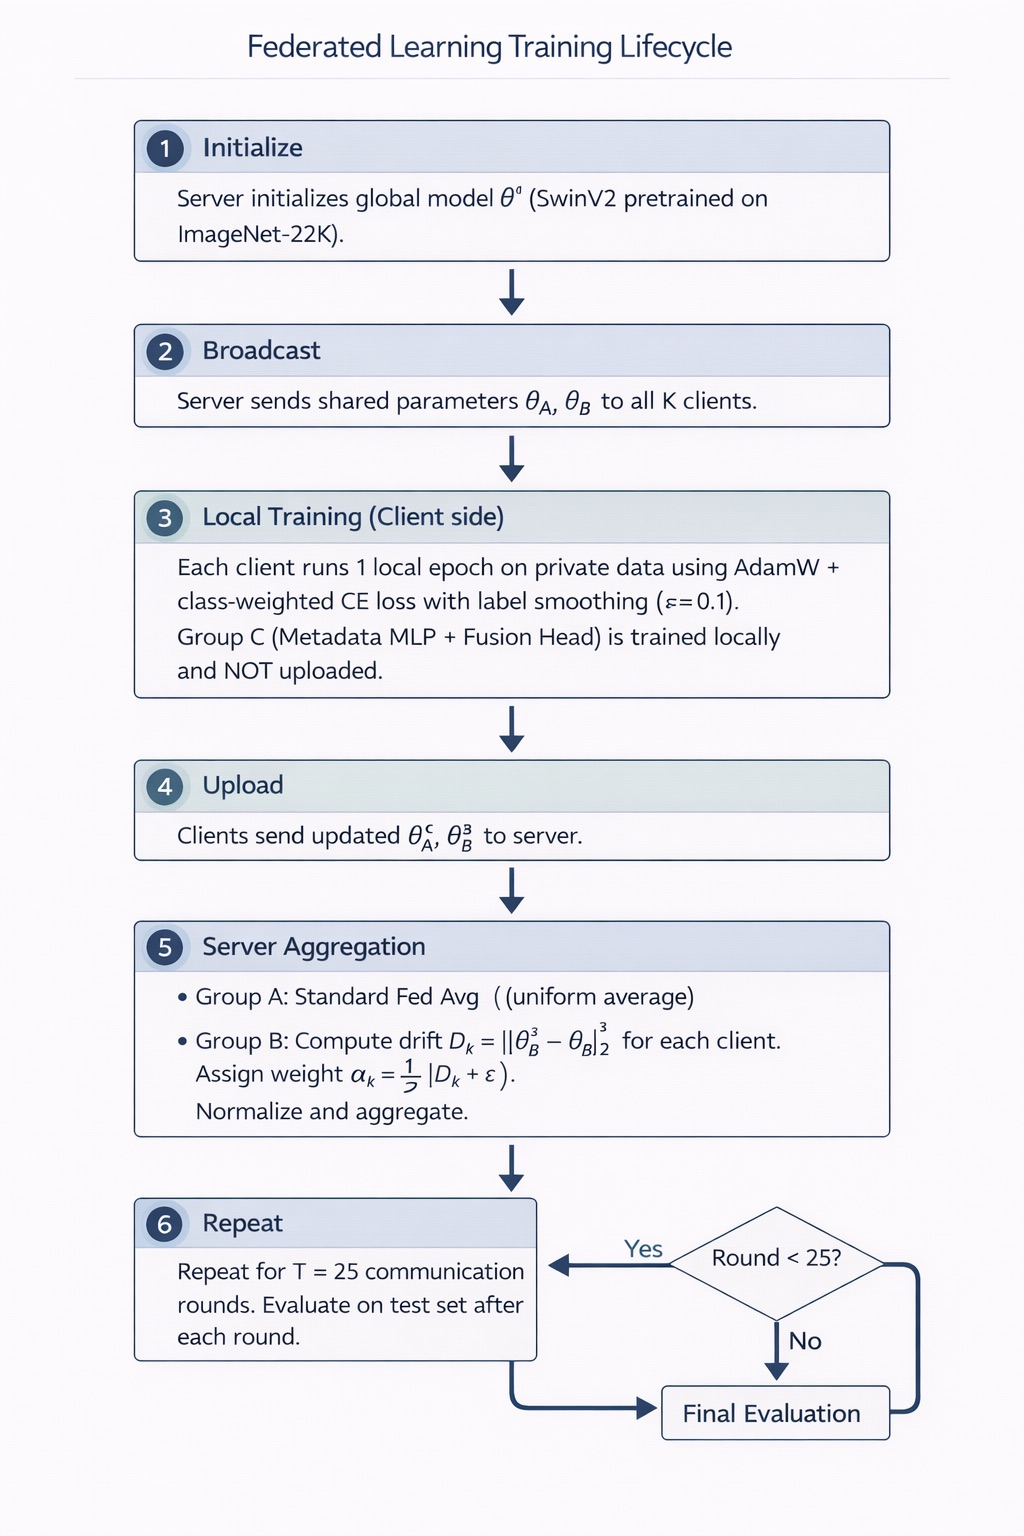
\includegraphics[width=0.72\columnwidth]{images/flowing.jpg}
\caption{Federated training lifecycle across communication rounds.}
\label{fig:flow}
\end{figure}
% Experiments

\subsection{Dataset}

\sadrift{} is evaluated on the ISIC 2019 dataset, which consists of 25,331 dermoscopic images that encompass eight categories: Melanoma (MEL), Melanocytic Nevus (NV), Basal Cell Carcinoma (BCC), Actinic Keratosis (AK), Benign Keratosis (BKL), Dermatofibroma (DF), Vascular Lesion (VASC) and Squamous Cell Carcinoma (SCC). The unknown \texttt{UNK} class was removed before training. A separate test set of 8,238 images is available for final evaluation.

\subsection{Data Accounting}
\label{sec:data_accounting}

Because several reported quantities depend on exactly which images are used where, we state the split arithmetic in full.

The ISIC 2019 training archive contains 25,331 labelled dermoscopic images across the eight classes. We hold out a stratified 15\% validation split of 3,800 images; the remaining \textbf{21,531} images form the training partition that is distributed across clients by the Dirichlet procedure. Summing the per-client class counts reported in Section~\ref{sec:severe_setting} reproduces this figure exactly ($1015 + 2687 + 11339 + 4945 + 1545 = 21{,}531$), and the per-class totals reconcile with the archive: for example melanoma contributes 3,844 images to the training partition and 678 to the validation split, together the 4,522 melanoma images the archive contains. No image appears in more than one split, although sibling images of the same lesion do; this is quantified in the Limitations section and bounds how the validation figures should be read.

The ISIC 2019 \emph{test} collection is a separate set of 8,238 images and is not drawn from the 25,331. Its released ground truth assigns 2,047 of those images to an \texttt{UNK} (outlier) category that lies outside our eight-class label space; since the model has no \texttt{UNK} output, these are excluded and all test-split results are computed on the remaining \textbf{6,191} labelled images. Melanoma accounts for 1,327 of them. These 1,327 test melanomas are distinct from the 4,522 in the training archive; the two collections are disjoint, and the melanoma counts should not be summed against the archive total.

One consequence is worth stating plainly. The centralized balanced accuracy of 0.8867 is measured on the internal validation split, which is drawn from the same archive as the training data. It is therefore not comparable with balanced accuracies reported on the ISIC 2019 test collection by challenge entries, and we do not present it as such. Our own test-split figures are substantially lower than our validation figures across every configuration---for example 0.3681 against 0.4382 for \sadrift{} at $\alpha{=}0.1$---which is the expected consequence of evaluating on a genuinely held-out collection.

The images are resized to $384 \times 384$ pixels and normalised using ImageNet statistics ($\mu = [0.485, 0.456, 0.406]$, $\sigma = [0.229, 0.224, 0.225]$). The augmentation applied to the training images varies and includes random resized crops, random horizontal and vertical flips, rotations up to 45\textdegree, color jittering, RandAugment (2 ops, magnitude 9) and random erasing ($p=0.3$). All augmentations are applied during the training process only.

\subsection{Federated Data Partitioning}

The 21,531 samples of the training partition (Section~\ref{sec:data_accounting}) are distributed across $K$ clients in accordance with a Dirichlet distribution centered at the concentration parameter $\alpha$. For instance, $\alpha = 1.0$ simulates near-IID conditions, $\alpha = 0.5$ simulates moderately heterogeneous class distributions, and $\alpha = 0.1$ simulates severe skew in which individual clients may hold no samples at all for several classes. All three values are evaluated in this work. Each client is allocated a minimum of 2 class labels and at least 100 samples. If the partition does not pass these criteria, a new random seed is attempted, for a maximum of 50 times.

\subsection{Model Architecture}

The model architecture consists of a SwinV2-Base (\texttt{swinv2\_base\_window12to24\_192to384}, pre-trained on ImageNet-22K) backbone combined with a metadata branch. The SwinV2-Base implements shifted-window self-attention using 4 hierarchical levels to produce a 1024-dimensional feature representation from images. A two-layer metadata MLP ($13 \to 128 \to 128$ with GELU activation and dropout) provides a 128-dimensional feature representation of the age, sex, and anatomical site of each patient. This gives a total of 1152 dimensions as a concatenation of 1024 dimensions from the images and 128 dimensions from the metadata. The combined 1152-dimensional representation is then input to a fusion head that reduces the representation from $1152 \to 512 \to 8$ to classify each lesion into one of eight categories.

\subsection{Training Protocol}

The centralized baseline is trained on the same 21,531-image training partition with no client split, for 25 epochs, and is evaluated on the same 3,800-image validation split. It therefore serves as an upper bound under identical data conditions, not as a comparison against externally reported numbers.

Using federated training, FedAvg is used as the baseline aggregation method. The process for each communication round is as follows:
\begin{enumerate}
    \item The global model is broadcast from the server to all $K$ clients.
    \item Each client performs local training on its own data.
    \item Each client uploads the parameters to the server for both Group A and Group B.
    \item The server combines the updates and sends out a new global model.
\end{enumerate}
A total of 25 communication rounds are completed. The local training loss is computed using class-weighted cross-entropy with label smoothing ($\epsilon_s = 0.1$):

\begin{equation}
\label{eq:local_loss}
\mathcal{L}_k = \mathcal{L}_{CE}^{\text{weighted}}(f_{\theta}(x^k, m^k),\, y^k)
\end{equation}

Both drift correction and aggregation updates are completed only at the server; therefore, all local training objectives remain unchanged.

\subsection{Optimization Details}

The AdamW optimizer is configured via hyperparameters ($\beta_1=0.9$, $\beta_2=0.999$, weight decay $10^{-2}$) with differential learning rates. The SwinV2 backbone uses $0.1\eta$, while $\eta = 4 \times 10^{-4}$ is used for the metadata MLP and the fusion head. The learning rate schedule consists of a cosine decay following a linear warmup of 2 epochs. Gradient clipping is applied so that gradients remain at most 1.0.

Each class is weighted by the inverse of its class frequency. At every round, the \texttt{WeightedRandomSampler} oversamples the low-frequency classes at each client. A single batch size of 32 (16 per optimizer step with 2 gradient accumulation steps (effective batch 32 on one device)) is used during centralized training. The batch size is set to 16 with 1 local epoch per round at each federated client.

All experiments were completed using FP16 mixed precision on a single NVIDIA A40 GPU with 48~GB of RAM. All federated experiments are simulated rather than deployed: clients are trained sequentially within a single process, so no network communication takes place. The $\alpha \in \{0.5, 1.0\}$ configurations were each run on one NVIDIA A40; the three $\alpha{=}0.1$ configurations were run concurrently on three A40s, one configuration per device, which affects wall-clock time only.

\subsection{Evaluation Metrics}

Two evaluation sets are used and are kept distinct throughout. Round-by-round metrics during training, and every figure reporting communication rounds, are computed on the 3,800-image \emph{validation} split. Results labelled \emph{test} are computed on the separate ISIC 2019 test collection, restricted to its 6,191 labelled images as described in Section~\ref{sec:data_accounting}. The following metrics are reported:
\begin{itemize}
    \item Top-1 Accuracy and Balanced Accuracy
    \item Macro F1-Score and Macro ROC-AUC
    \item Macro Average Precision
    \item Per-class classification report and confusion matrix
\end{itemize}

In addition to the above metrics, fairness evaluation is performed using:
\begin{itemize}
    \item Worst-case client accuracy (minimum across all clients)
    \item Inter-client standard deviation of accuracy
\end{itemize}
Every dispersion percentage reported in this paper is a reduction in this \emph{standard deviation}, not in its square. For reference, a 39\% reduction in standard deviation corresponds to a 62.4\% reduction in variance; we quote the former throughout.

\section{Results and Discussion}

The performance of \sadrift{} is assessed along three dimensions: global classification accuracy, worst-client fairness and computational efficiency. Numerical comparisons with recent state-of-the-art methods are also provided.

\subsection{Centralized Upper Bound Performance}

\sadrift{} was trained in a centralized fashion on the 21,531-image training partition for 25 epochs, reaching a peak Balanced Accuracy of \textbf{0.8867} at Epoch~21 on the internal validation split. This figure serves only as a reference ceiling obtained under data conditions identical to the federated runs. It is not a generalization estimate: the validation split shares lesions with the training partition (see Limitations), and it is not comparable with balanced accuracies reported on the official ISIC 2019 test collection. Top-1 Accuracy at this point was 0.8566, Macro ROC-AUC was 0.9607 and Macro F1-score was 0.8237. Epoch~21 is the maximum rather than the onset of a plateau: balanced accuracy is lower at Epochs 22--25. We also note that this epoch is selected on the same validation split on which the figure is reported, so 0.8867 is an optimistically selected value and is used here only as a reference ceiling under matched data conditions. Training curves can be found in Figure~\ref{fig:centralized_curves}. The terminal output is also available in Figure~\ref{fig:cent_terminal}.

The centralized baseline is reported here only as an internal reference ceiling; we make no comparison against externally reported figures, for the reasons given in Section~\ref{sec:data_accounting} and the Limitations.

\begin{figure*}[t]
\centering
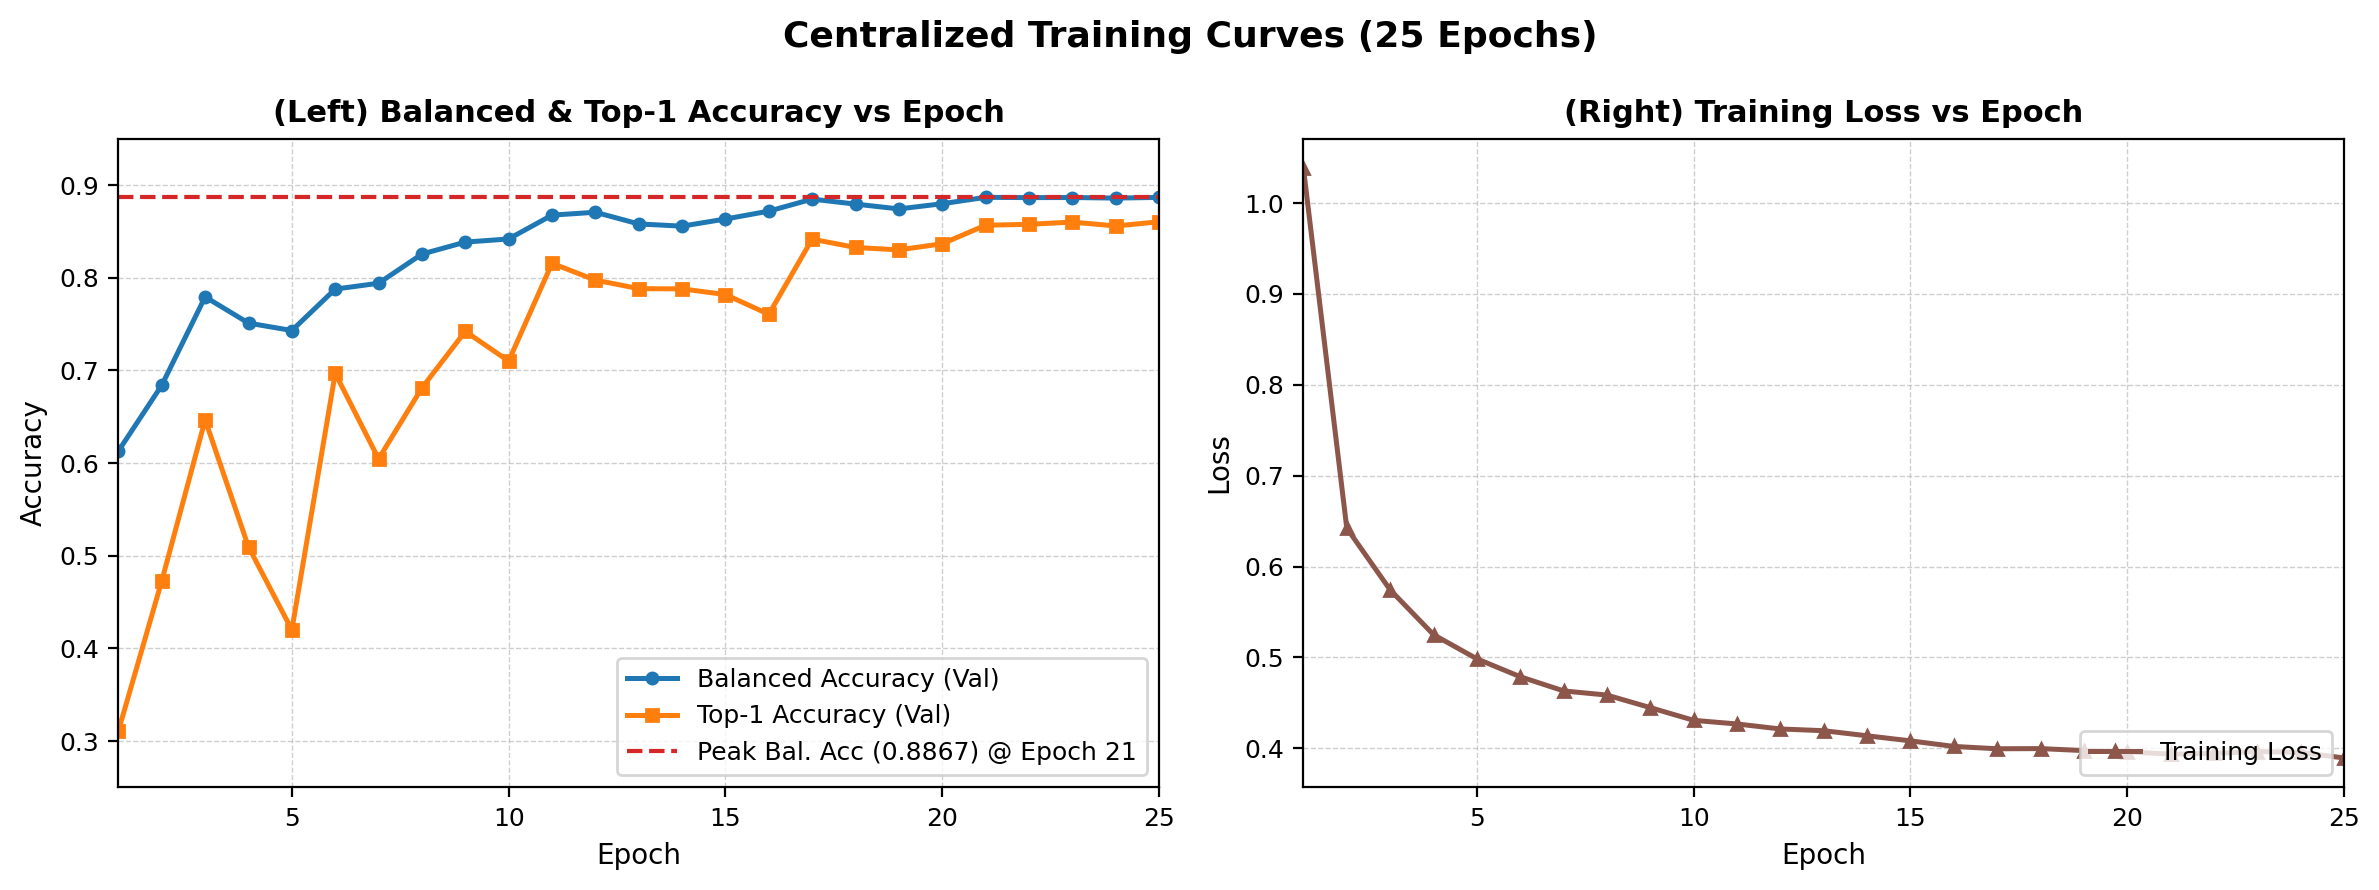
\includegraphics[width=\textwidth]{images/centralized_training_curves.png}
\caption{Centralized training curves over 25 epochs: (Left) Balanced Accuracy and Top-1 Accuracy; (Right) Training Loss. Peak Balanced Accuracy of 0.8867 is reached at Epoch~21.}
\label{fig:centralized_curves}
\end{figure*}

\begin{figure*}[t]
\centering
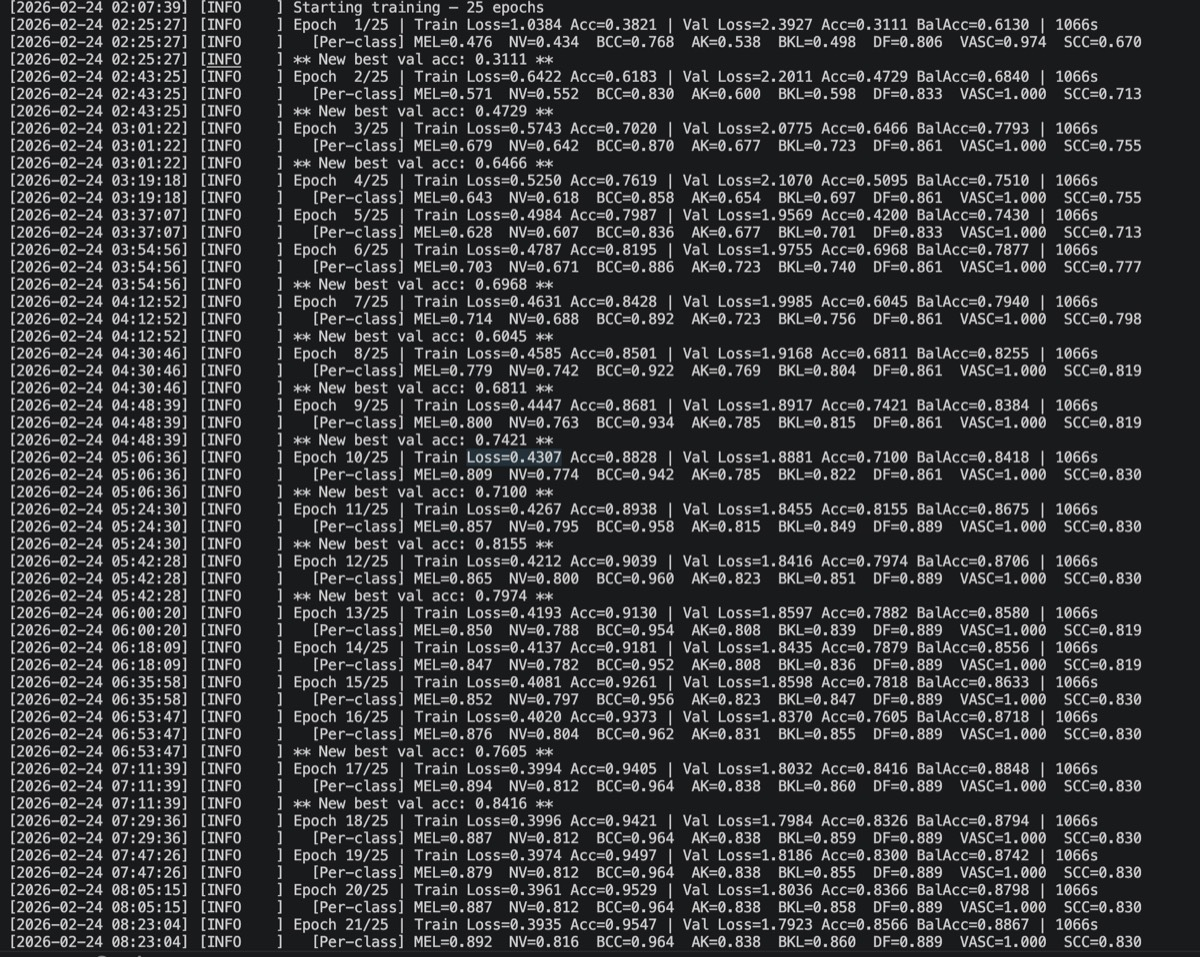
\includegraphics[width=0.80\textwidth]{images/centralized-run1.jpg}\\[4pt]
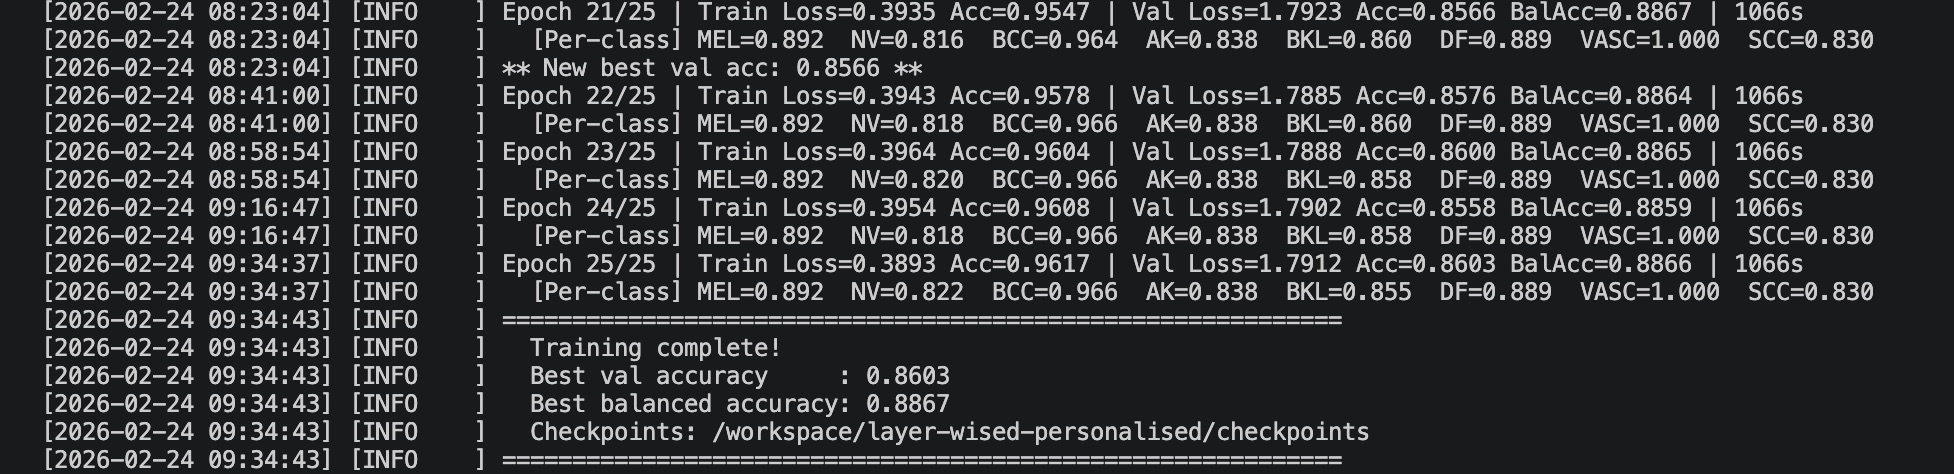
\includegraphics[width=0.80\textwidth]{images/centralized-run2.jpg}
\caption{Centralized training run terminal output (NVIDIA A40, RunPod): (Top) Epochs~1--13 showing progressive improvement in validation Balanced Accuracy; (Bottom) Epochs~14--25 converging to peak Balanced Accuracy of 0.8867 at Epoch~21, with per-class recall and final training summary.}
\label{fig:cent_terminal}
\end{figure*}

\subsection{Consolidated Federated Performance}

The results from each experimental configuration have been summarized in Table~\ref{tab:consolidated_performance}. These summary results consist of the centralized upper bound together with the three levels of Dirichlet heterogeneity ($\alpha \in \{1.0, 0.5, 0.1\}$) and the aggregation schemes evaluated at each, including the no-decomposition FedAvg baseline added at $\alpha{=}0.1$. All comparisons made after this step reference Table~\ref{tab:consolidated_performance}.

\begin{table*}[t]
\centering
\caption{Consolidated Performance of \sadrift{} Across All Experimental Configurations}
\label{tab:consolidated_performance}
\begin{tabular}{llccccc}
\toprule
Experiment & Config ($\alpha$, $K$) & Drift Strategy & Global Bal.\ Acc & Worst Client Acc & Std Dev (Acc) & Avg Round Time \\
\midrule
Centralized & N/A & N/A & 0.8867 & N/A & N/A & 1066\,s \\
Fed-2 (Baseline) & $\alpha{=}1.0$, $K{=}3$ & Uniform (Off) & \textbf{0.8314} & 0.6479 & 0.0182 & 1297\,s \\
Fed-1 (Ours) & $\alpha{=}1.0$, $K{=}3$ & Adaptive (On) & 0.8209 & \textbf{0.7850} & \textbf{0.0076} & 1301\,s \\
Fed-4 (Baseline) & $\alpha{=}0.5$, $K{=}5$ & Uniform (Off) & \textbf{0.7622} & 0.4800 & 0.0833 & 1439\,s \\
Fed-3 (Ours) & $\alpha{=}0.5$, $K{=}5$ & Adaptive (On) & 0.7066 & \textbf{0.5705} & \textbf{0.0511} & 1450\,s \\
\midrule
Fed-7 (FedAvg)\textsuperscript{$\dagger$} & $\alpha{=}0.1$, $K{=}5$ & No decomposition & 0.4460 & --- & --- & 1229\,s \\
Fed-6 (Baseline) & $\alpha{=}0.1$, $K{=}5$ & Uniform (Off) & 0.4477 & 0.1953 & 0.1294 & 1398\,s \\
Fed-5 (Ours) & $\alpha{=}0.1$, $K{=}5$ & Adaptive (On) & \textbf{0.5196} & \textbf{0.4297} & \textbf{0.0551} & 1397\,s \\
\bottomrule
\end{tabular}

\vspace{2pt}
{\footnotesize \textsuperscript{$\dagger$}Fed-7 removes the A/B/C decomposition entirely, so no client-specific head exists and every client evaluates an identical model; worst-client accuracy and inter-client dispersion are undefined for this configuration rather than favourable. Its Global Bal.\ Acc is also the only entry in this column produced by a fully aggregated network: for the decomposed arms the shared model carries the common initial Group~C head rather than an aggregated one (see Limitations). The column is comparable within the decomposed family but not across it; Table~\ref{tab:threeway} gives the like-for-like per-client comparison.}
\end{table*}

\subsection{Mitigating Exacerbated Drift and Ensuring Client Fairness}

In multimodal federated networks that keep metadata heads local but share a common backbone, client drift can be exacerbated as the visual backbone is driven toward different local optima \cite{Zhu2025}. This paper confirms this through experiments with \sadrift{} and describes it in more detail below.

\subsubsection{Near-IID Setting ($\alpha = 1.0$, $K = 3$)}

With $K{=}3$ clients and $\alpha{=}1.0$, the class distributions are nearly uniform across clients. Two different aggregation methodologies are compared: 1) standard FedAvg, and 2) \sadrift{} that uses drift-aware weighting on Group~B.

Under these mild levels of client heterogeneity, FedAvg achieves a balanced global accuracy of 0.8314; however, the worst-performing client drops to 0.6479, which would not be apparent from the global average. Using \sadrift{}, the worst-client accuracy increases by \textbf{+13.71 points} to 0.7850, and the inter-client standard deviation decreases by \textbf{58\%} from 0.0182 to 0.0076 (observed in a single experimental trial). Measured on the shared global model, \sadrift{} reaches 92.6\% and the uniform-aggregation baseline 93.8\% of the centralized balanced accuracy, both on the same internal validation split.

The round-by-round training curves and terminal outputs (Figures~\ref{fig:near_iid_sadrift_bundle} and~\ref{fig:near_iid_fedavg_bundle}) clearly demonstrate that the two methodologies converge toward the centralized upper bound, and that \sadrift{} achieves a tighter client accuracy band and a higher worst-client floor compared to FedAvg.

\begin{figure*}[!t]
\centering
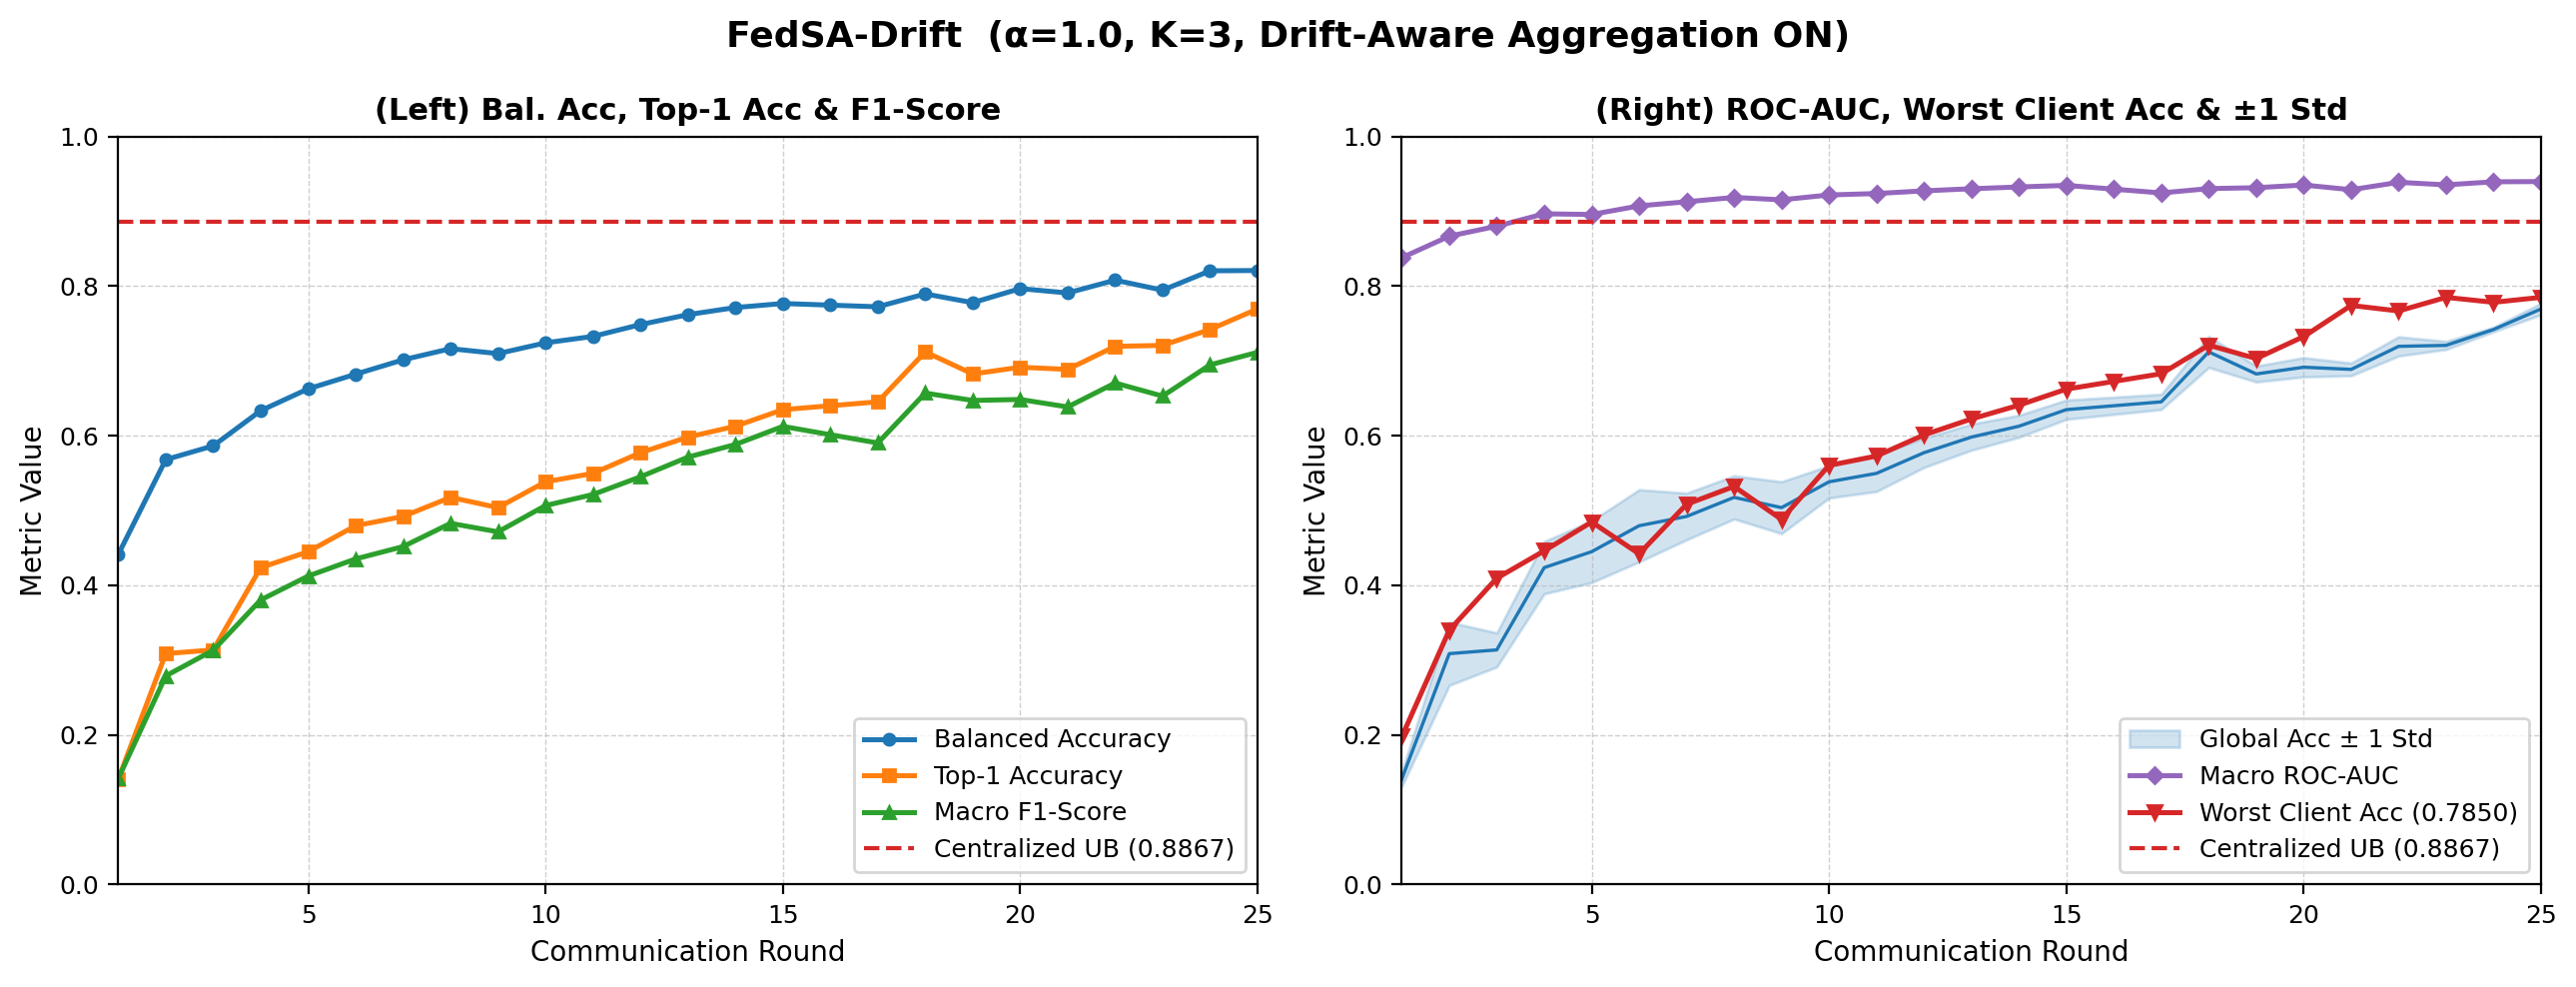
\includegraphics[width=0.80\textwidth]{images/sa_drift_near_iid_curves.png}\\[4pt]
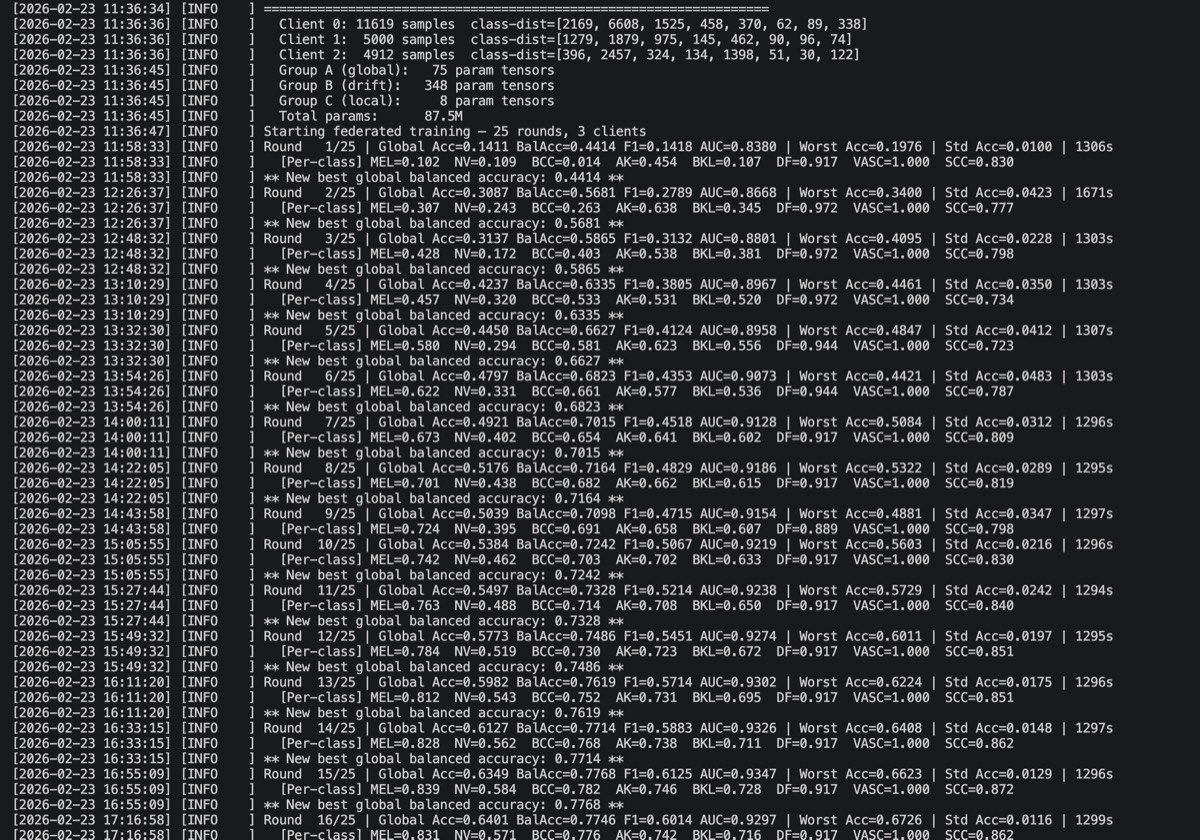
\includegraphics[width=0.80\textwidth]{images/a=1, client=3, drift= True1.jpg}\\[4pt]
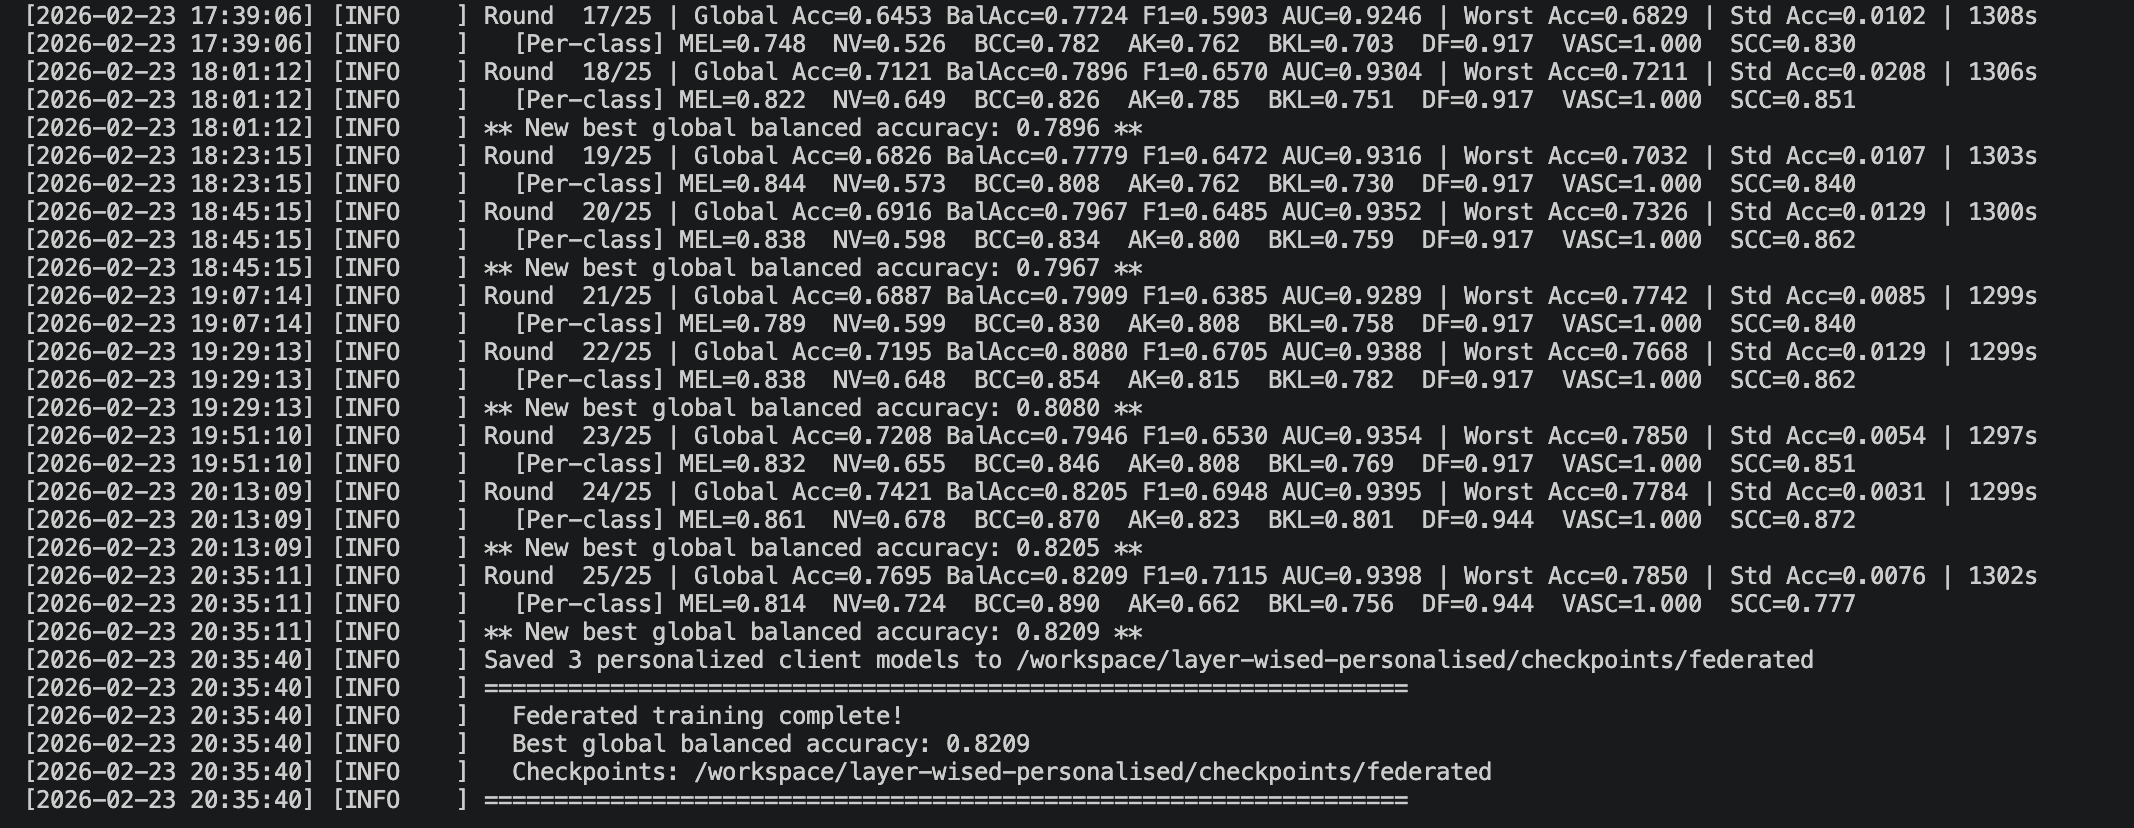
\includegraphics[width=0.80\textwidth]{images/a=1, client=3, drift= True2.png}
\caption[FedSA-Drift near-IID (alpha=1.0, K=3)]{FedSA-Drift near-IID setting ($\alpha{=}1.0$, $K{=}3$): top panel shows convergence metrics; middle and bottom panels show terminal outputs (Rounds 1--13 and 14--25). Final Balanced Accuracy: 0.8209, Worst Client Accuracy: 0.7850.}
\label{fig:near_iid_sadrift_bundle}
\end{figure*}

\begin{figure*}[!t]
\centering
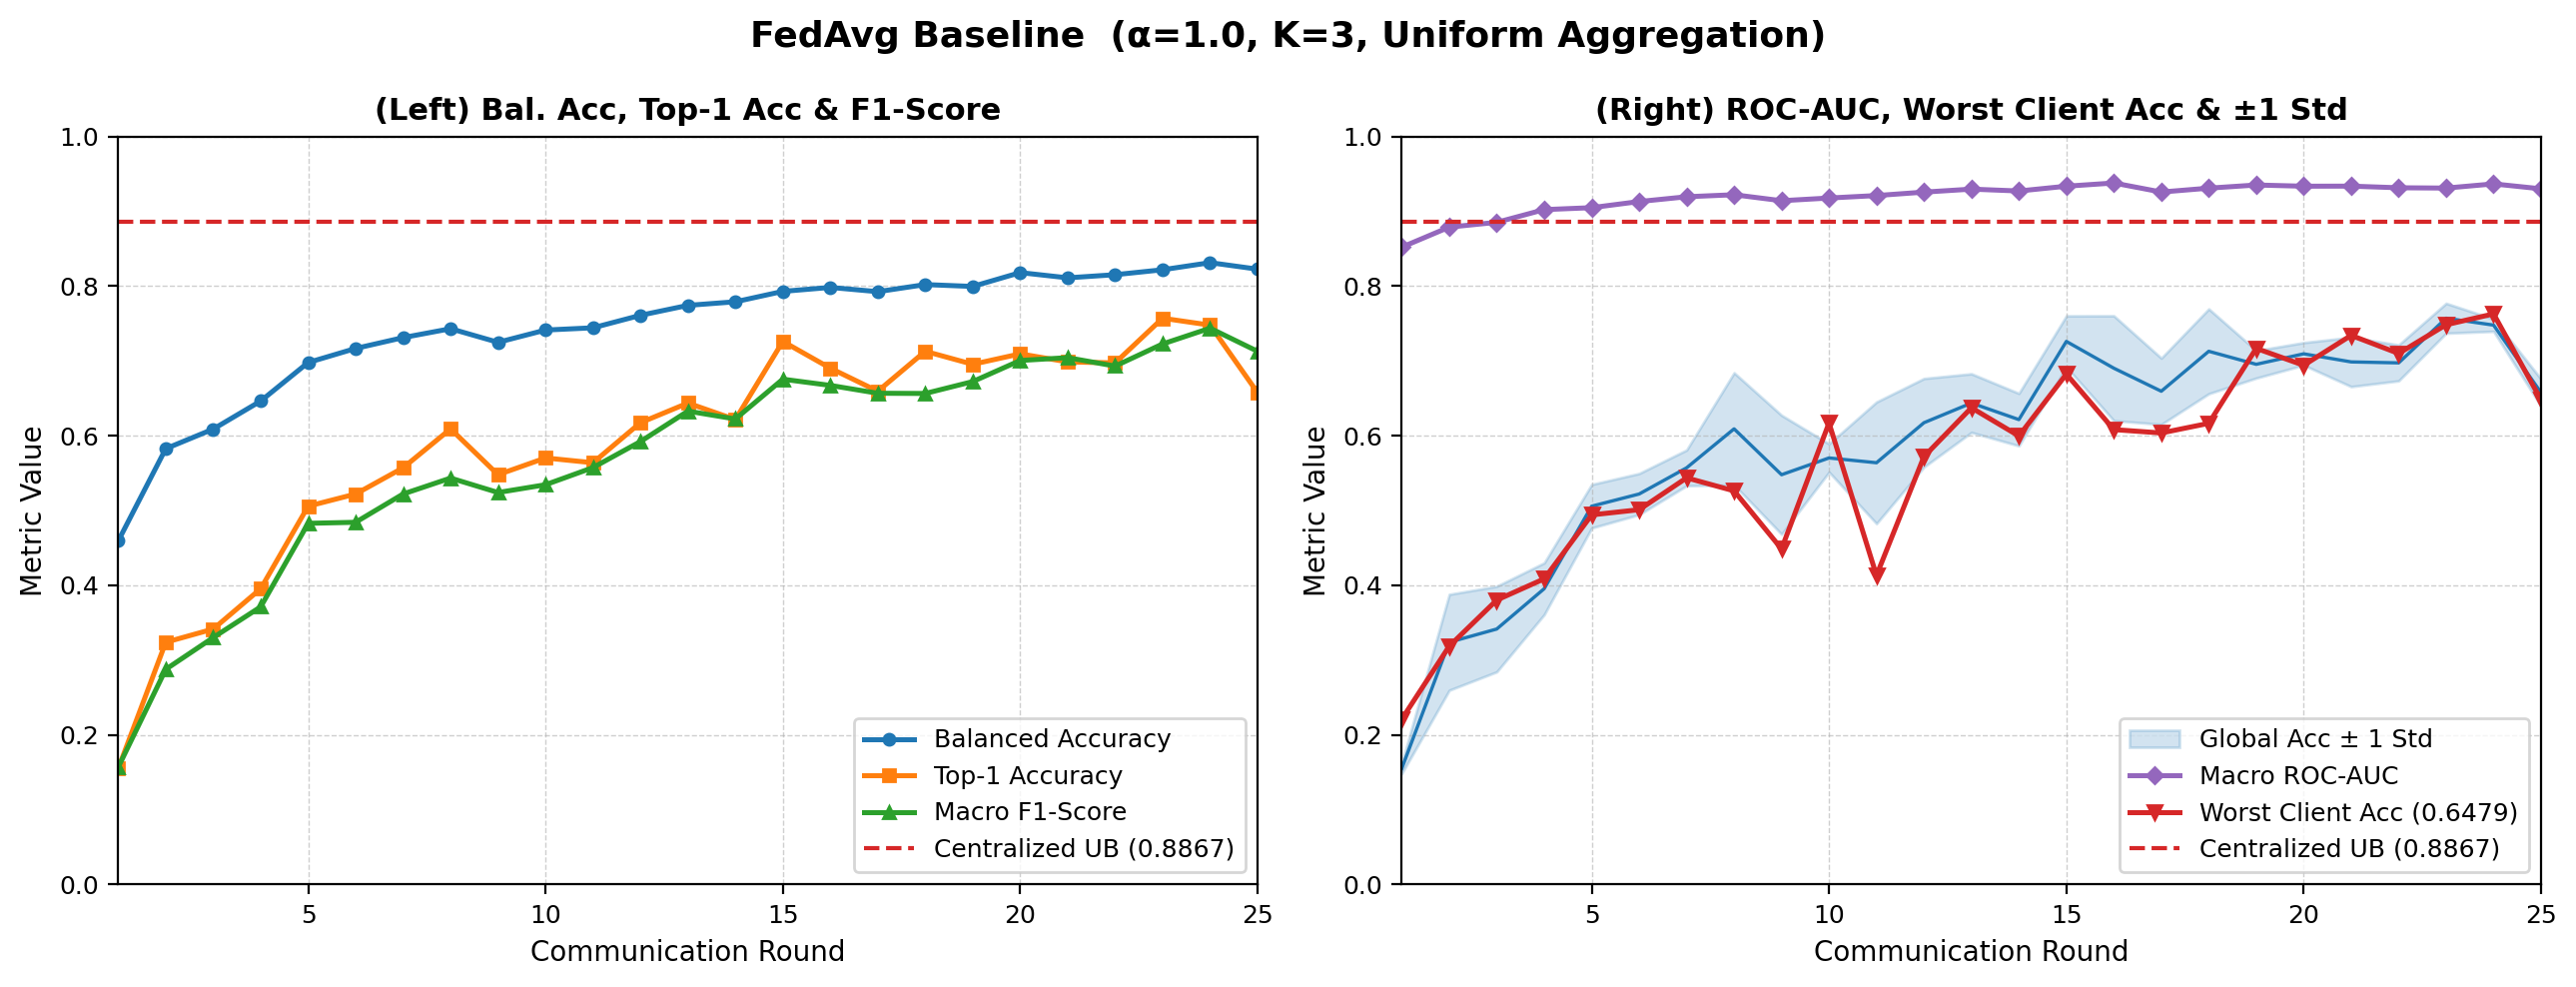
\includegraphics[width=0.80\textwidth]{images/fedavg_near_iid_curves.png}\\[4pt]
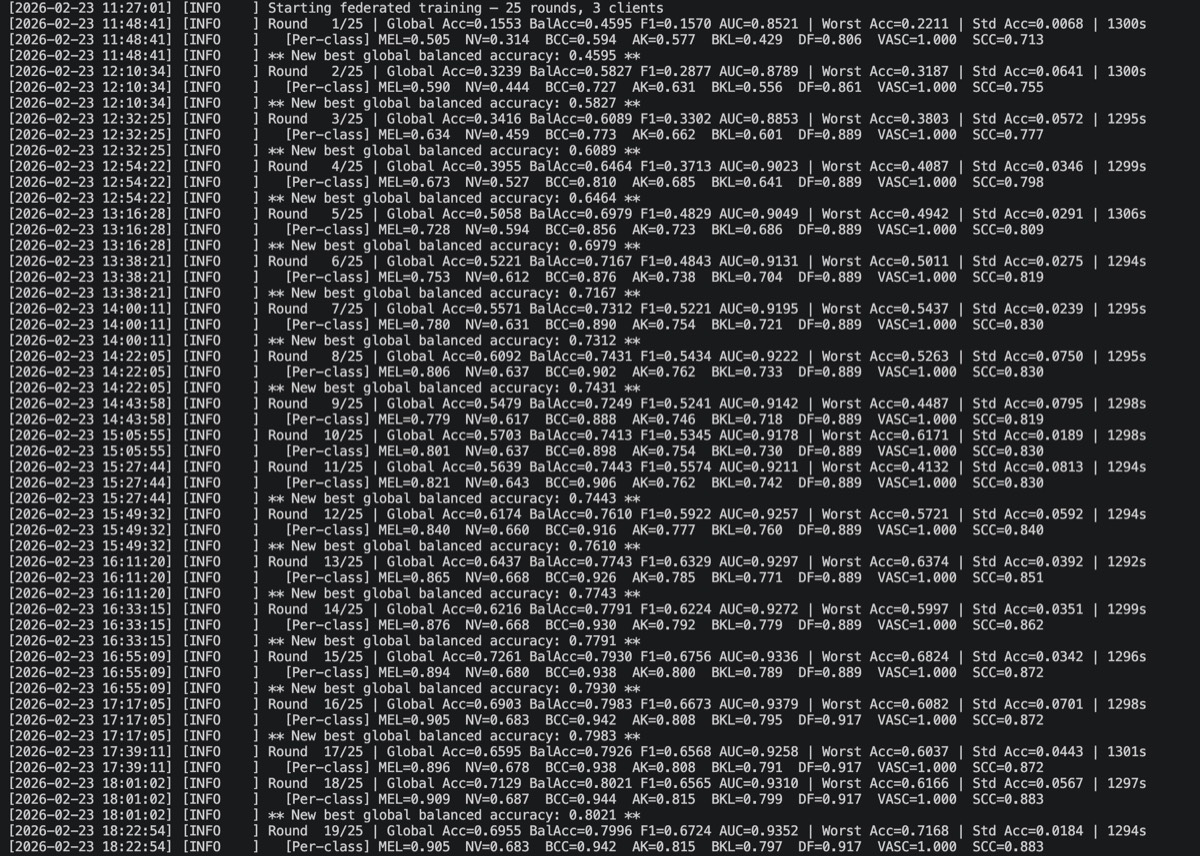
\includegraphics[width=0.80\textwidth]{images/a=1, client=3, drift= False1.jpg}\\[4pt]
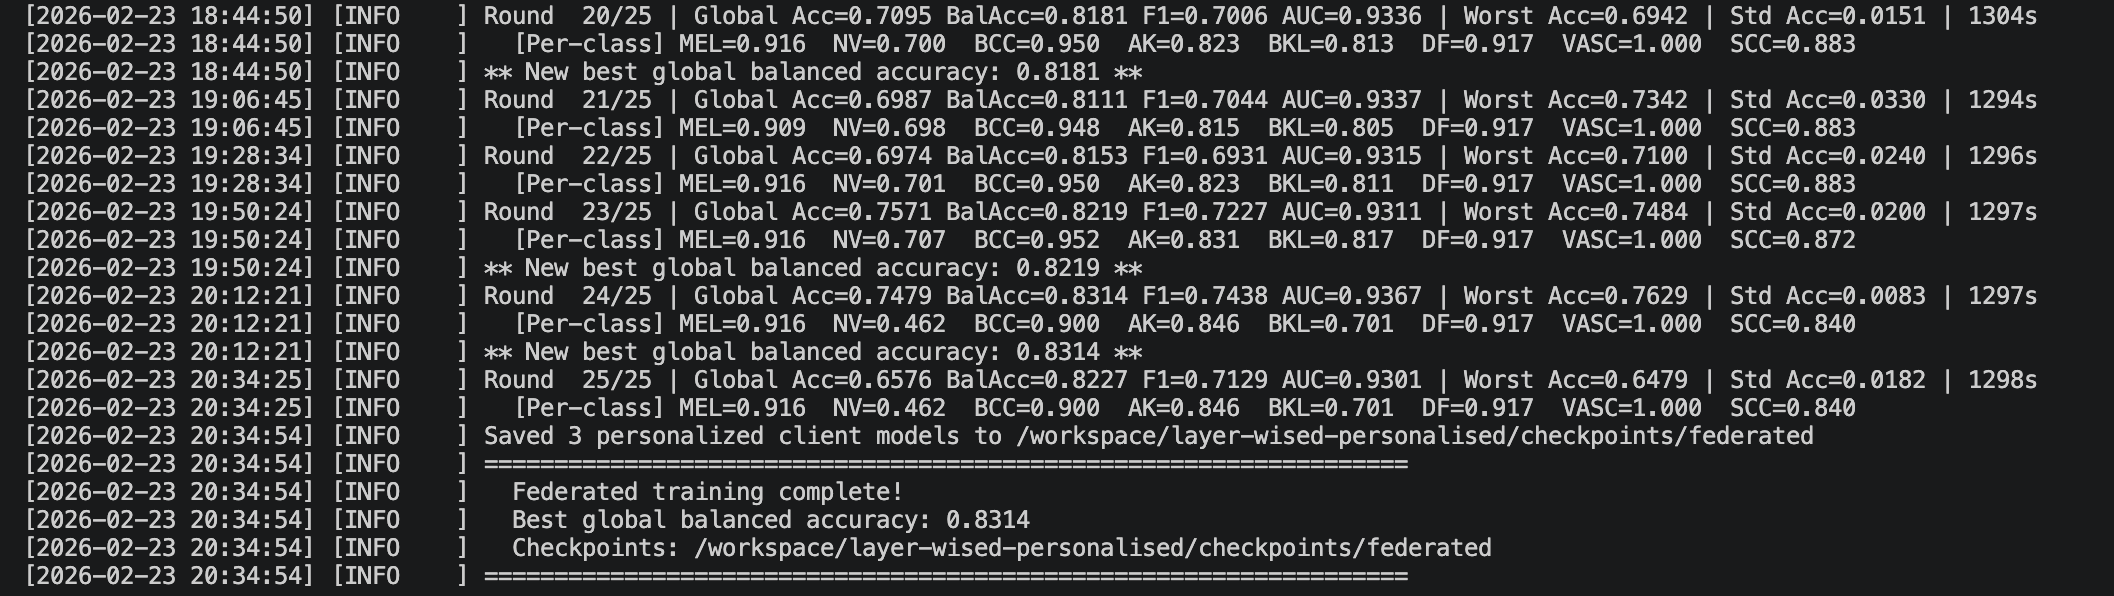
\includegraphics[width=0.80\textwidth]{images/a=1, client=3, drift= False2.png}
\caption[FedAvg near-IID (alpha=1.0, K=3)]{FedAvg near-IID setting ($\alpha{=}1.0$, $K{=}3$): top panel shows convergence metrics; middle and bottom panels show terminal outputs (Rounds 1--13 and 14--25). Final Balanced Accuracy: 0.8314, Worst Client Accuracy: 0.6479.}
\label{fig:near_iid_fedavg_bundle}
\end{figure*}

\subsubsection{Moderately Heterogeneous Setting ($\alpha = 0.5$, $K = 5$)}

The introduction of significant class imbalance across institutions ($K{=}5$ and $\alpha{=}0.5$) produces a more realistic clinical scenario. The use of \sadrift{} to correct for drift provides an improvement over the worst client (lowest accuracy) of \textbf{+9.05 percentage points} from 0.4800 to 0.5705 and reduces the inter-client standard deviation of accuracy by \textbf{38.7\%} from 0.0833 to 0.0511 (observed in a single experimental trial). The results in Figures~\ref{fig:non_iid_sadrift_bundle} and~\ref{fig:non_iid_fedavg_bundle} indicate that the convergence of the different model types will be slower and noisier than in the near-IID case. Therefore, the improvement to the performance floor is clearly visible in this comparison.

\begin{figure*}[!t]
\centering
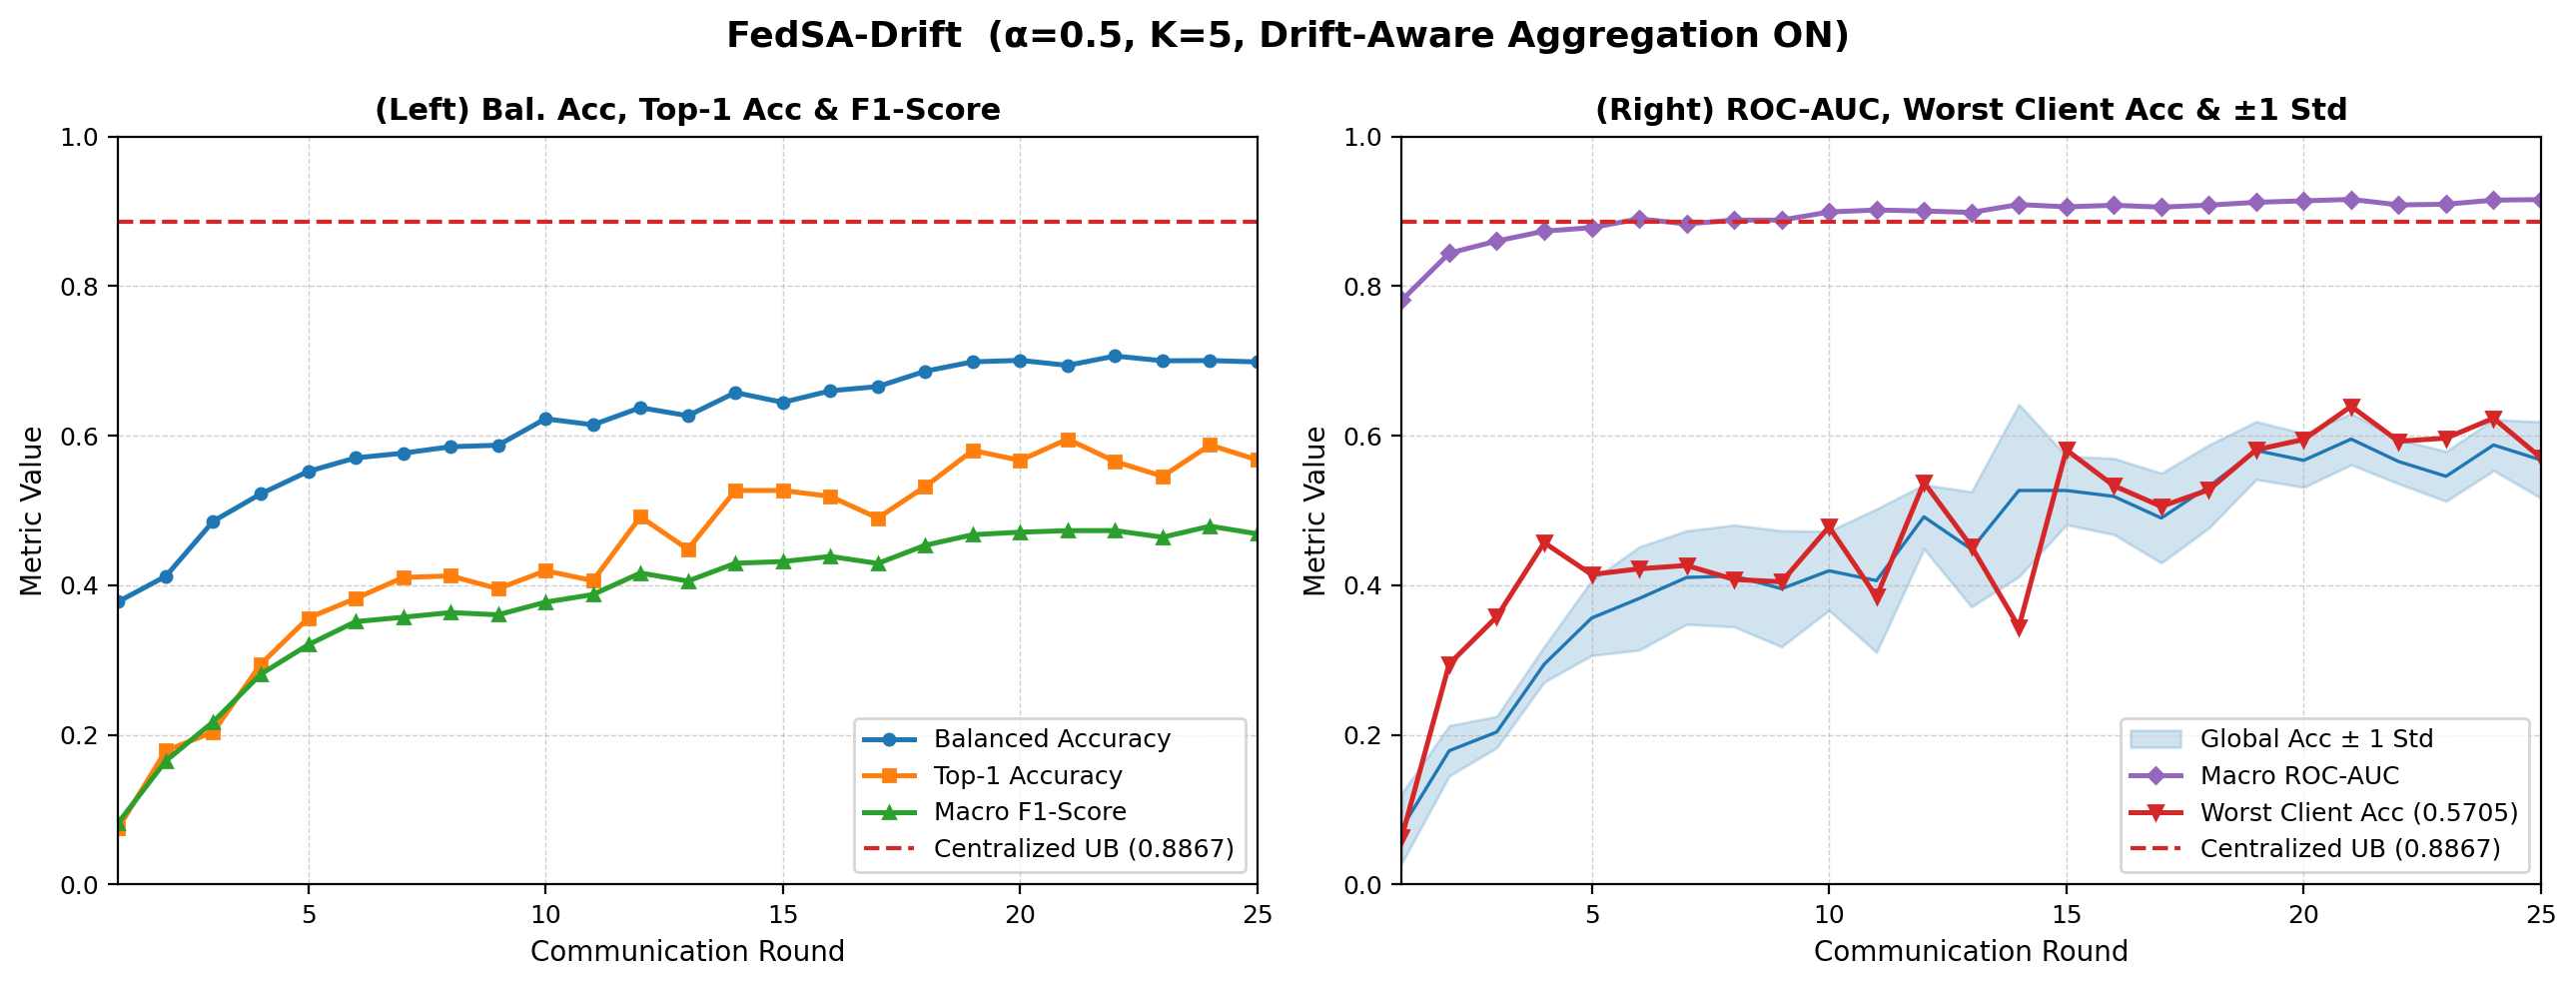
\includegraphics[width=0.80\textwidth]{images/sa_drift_non_iid_curves.png}\\[4pt]
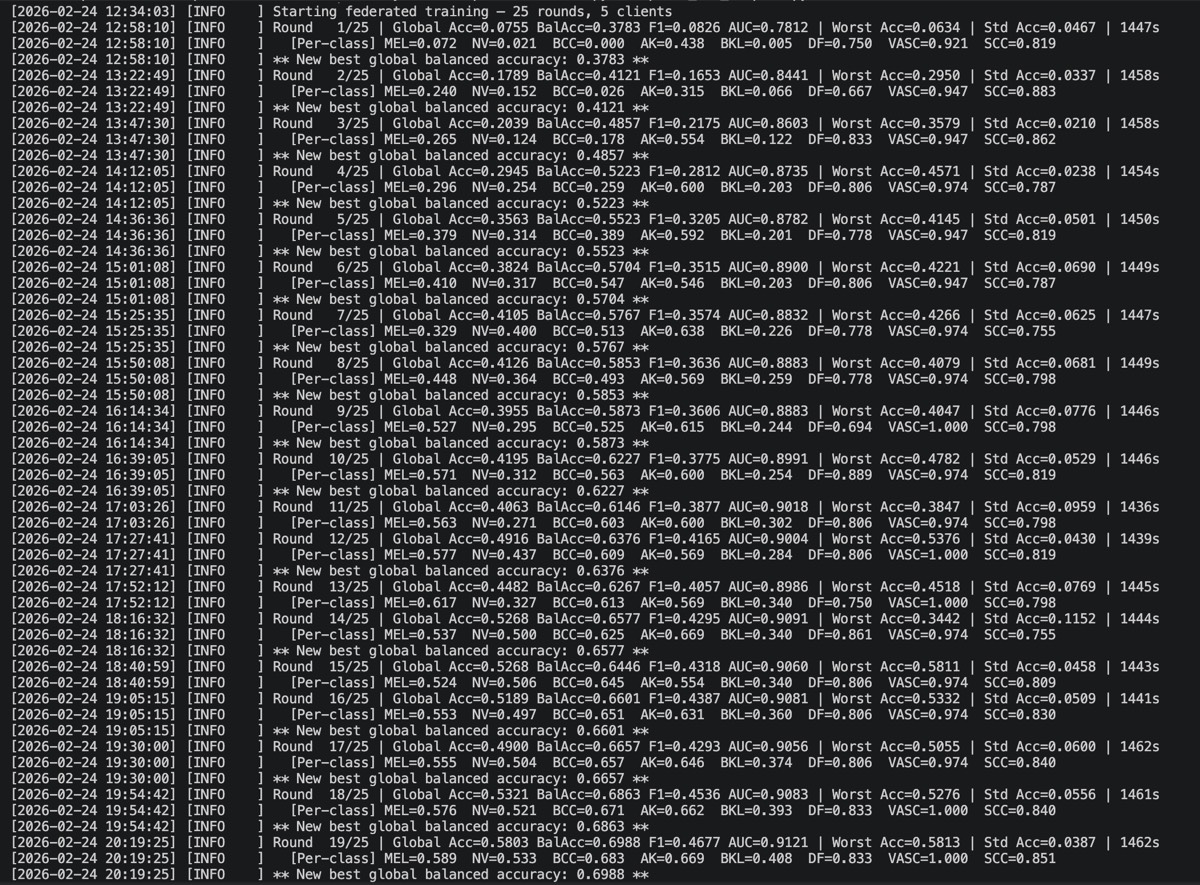
\includegraphics[width=0.80\textwidth]{images/a=0.5, client=5, drift= True1.jpg}\\[4pt]
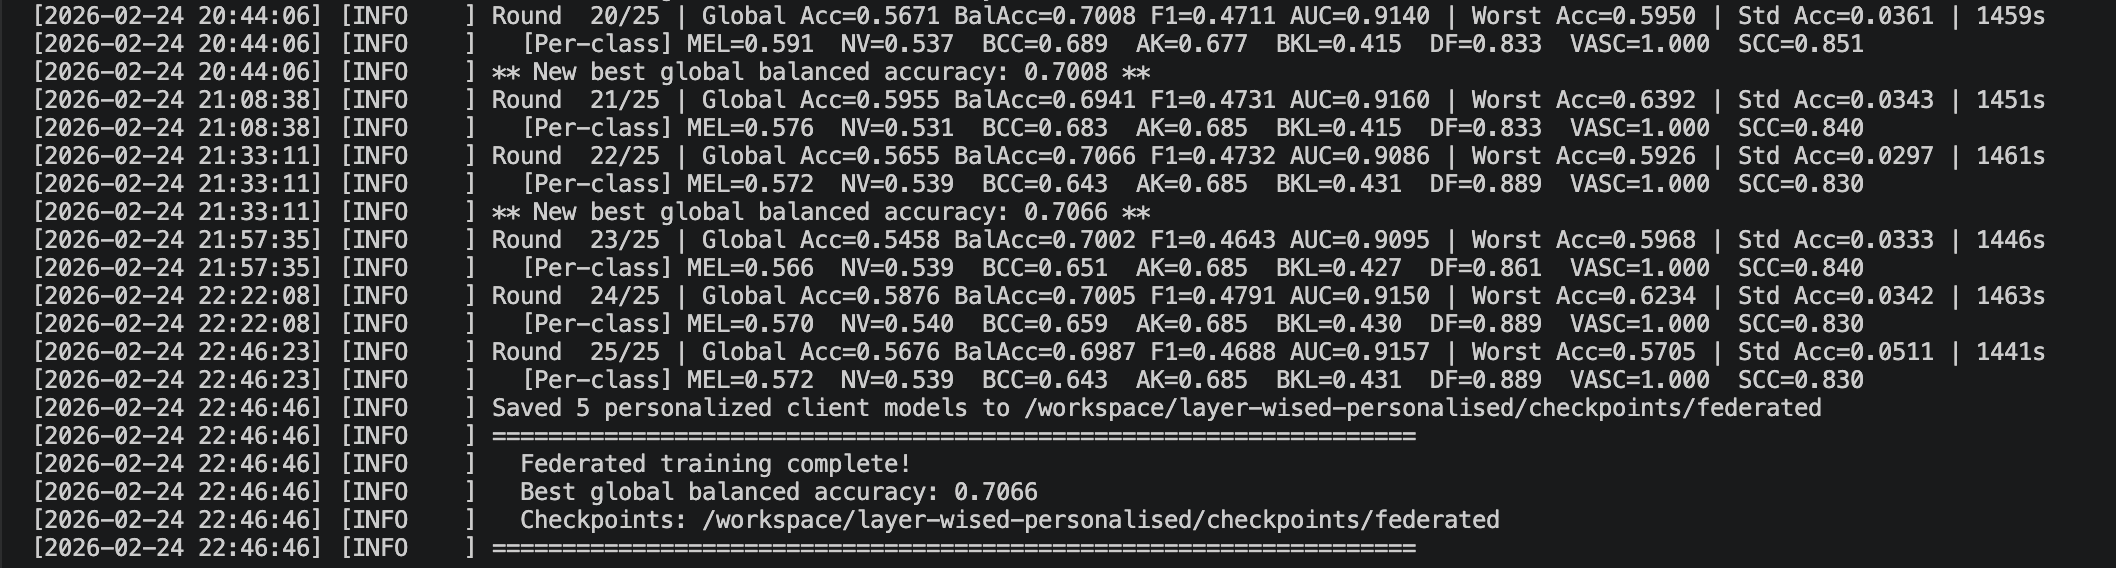
\includegraphics[width=0.80\textwidth]{images/a=0.5, client=5, drift= True2.png}
\caption[FedSA-Drift non-IID (alpha=0.5, K=5)]{FedSA-Drift non-IID setting ($\alpha{=}0.5$, $K{=}5$): top panel shows convergence metrics; middle and bottom panels show terminal outputs (Rounds 1--13 and 14--25). Final Balanced Accuracy: 0.7066, Worst Client Accuracy: 0.5705.}
\label{fig:non_iid_sadrift_bundle}
\end{figure*}

\begin{figure*}[!t]
\centering
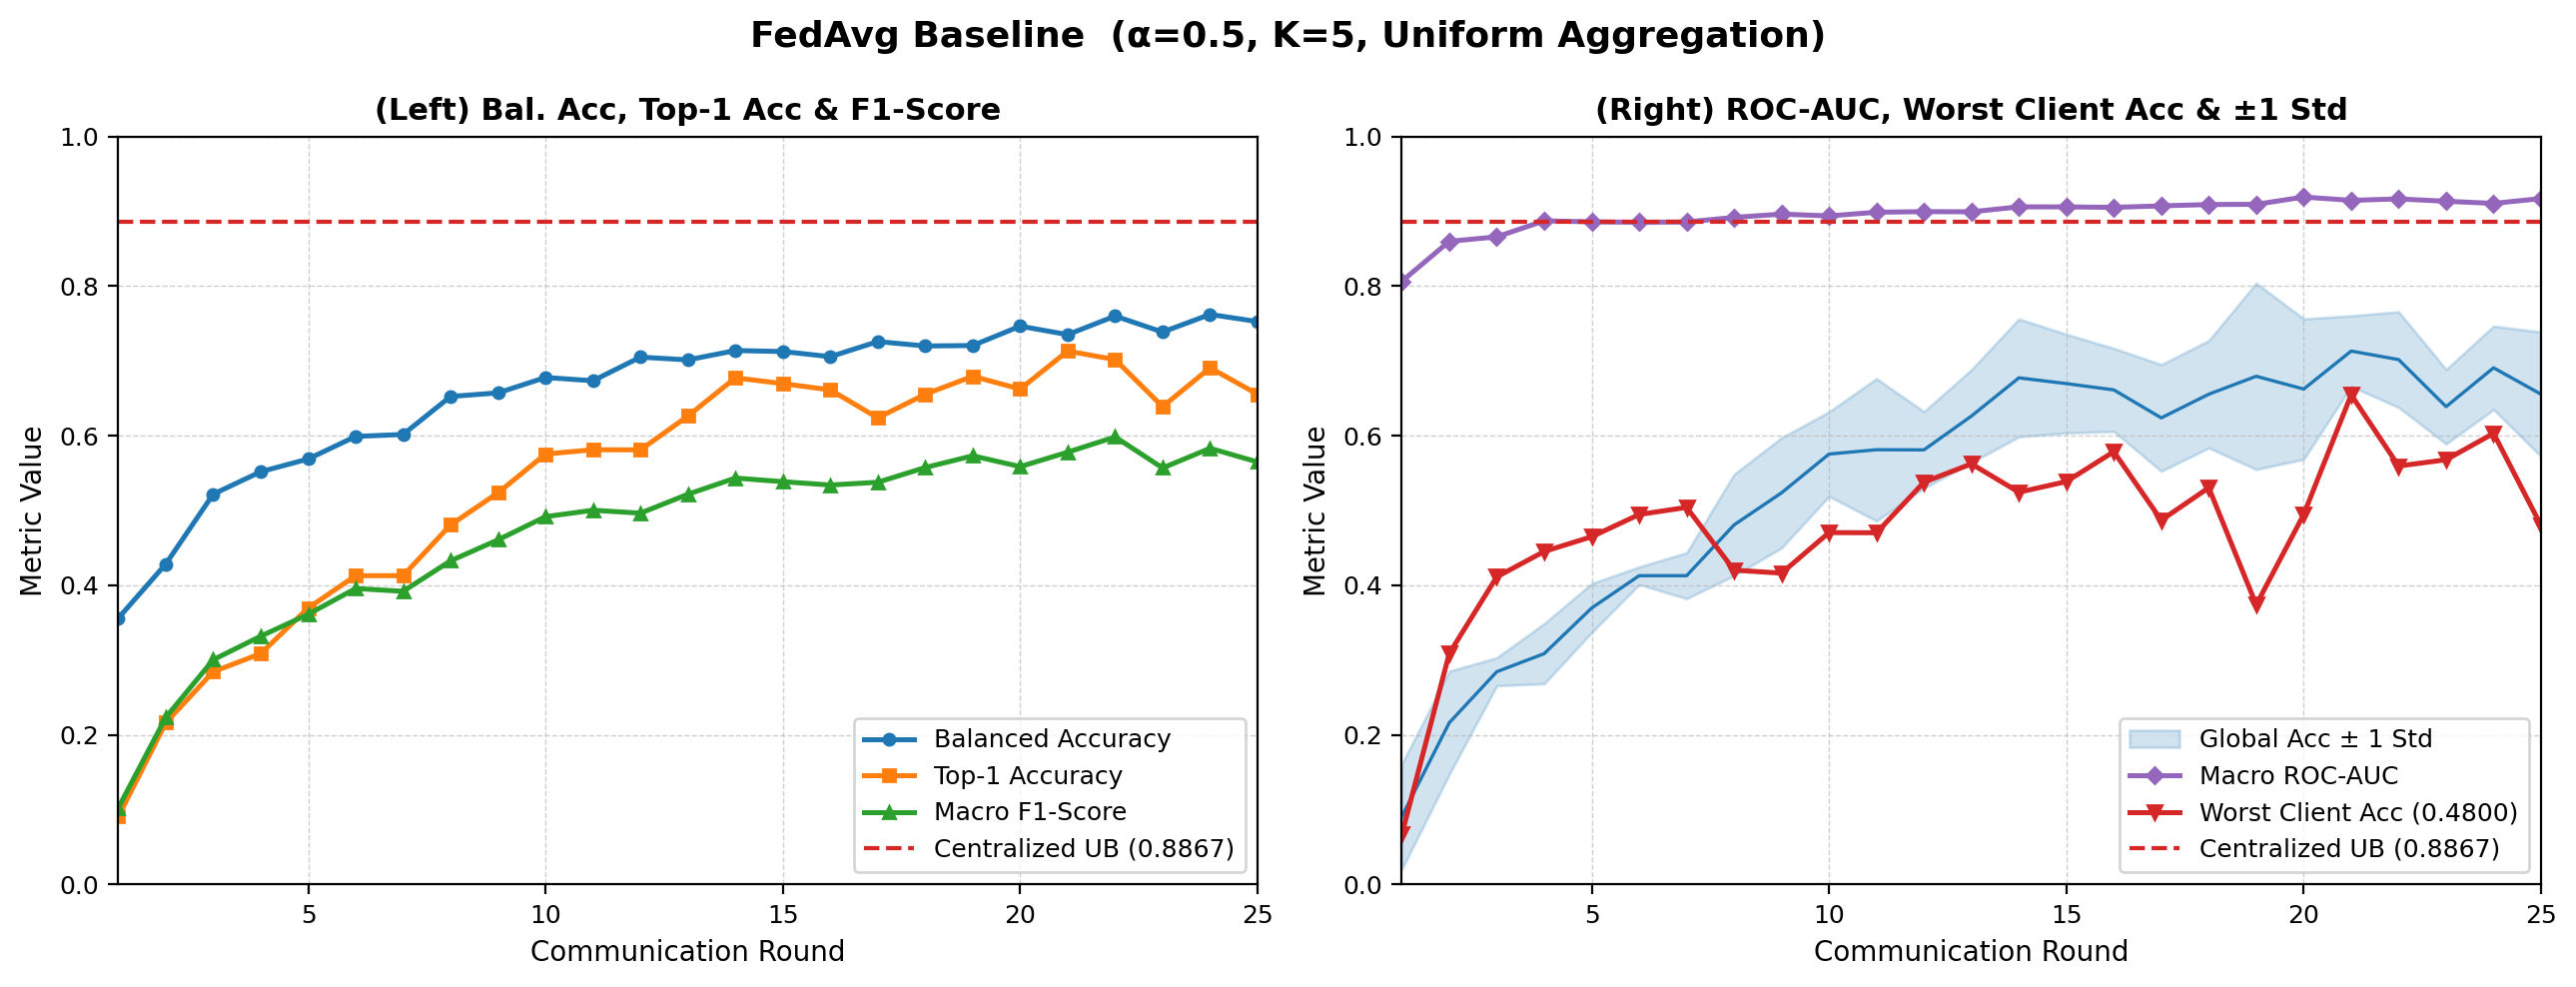
\includegraphics[width=0.80\textwidth]{images/fedavg_non_iid_curves.png}\\[4pt]
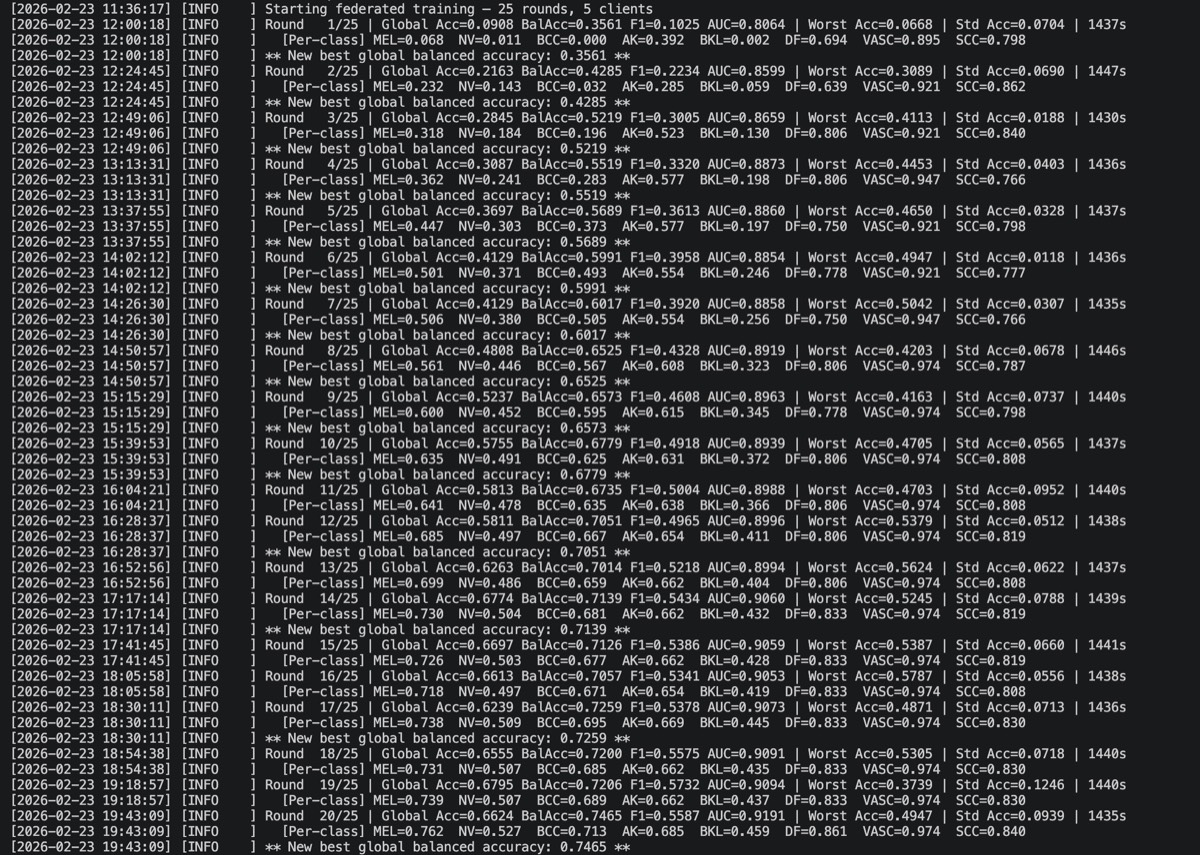
\includegraphics[width=0.80\textwidth]{images/a=0.5, client=5, drift= False1.jpg}\\[4pt]
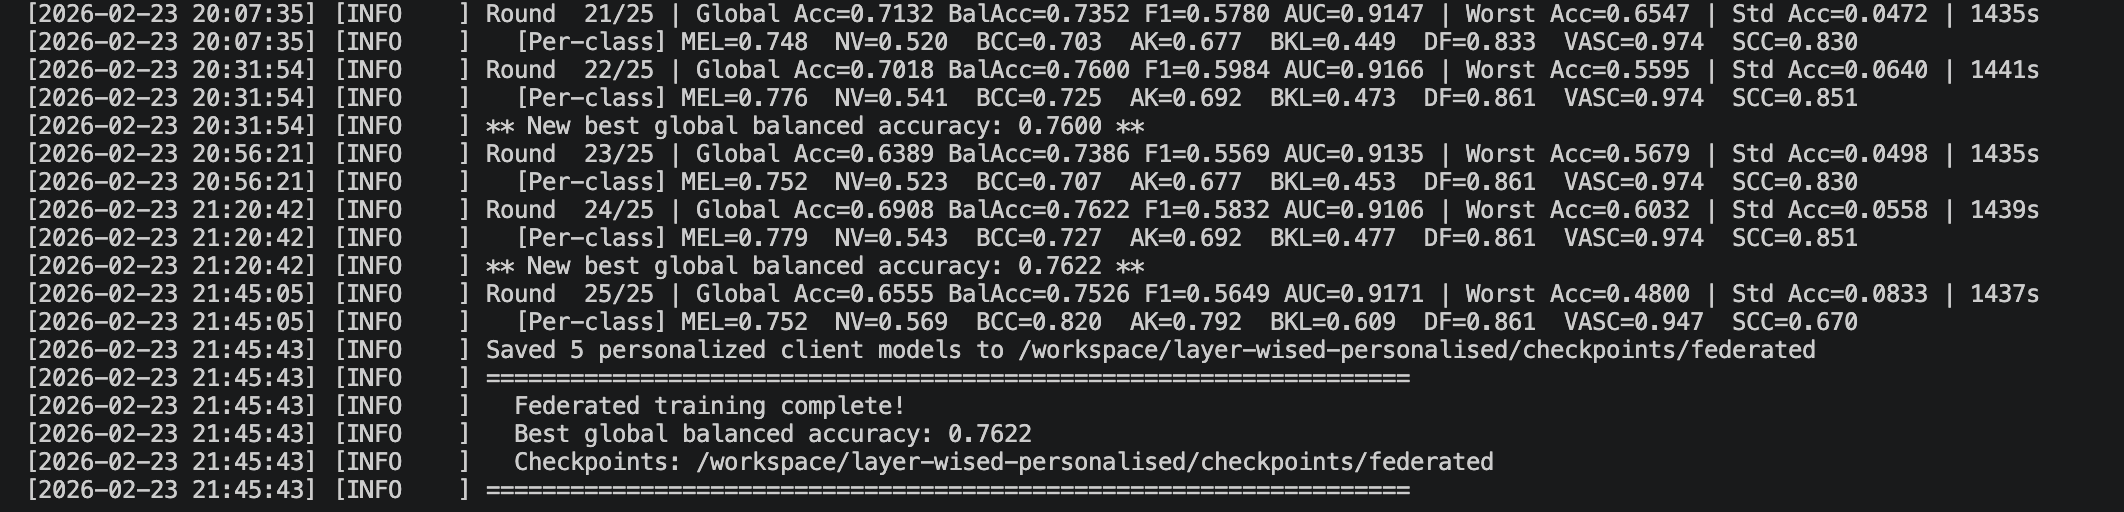
\includegraphics[width=0.80\textwidth]{images/a=0.5, client=5, drift= False2.png}
\caption[FedAvg non-IID (alpha=0.5, K=5)]{FedAvg non-IID setting ($\alpha{=}0.5$, $K{=}5$): top panel shows convergence metrics; middle and bottom panels show terminal outputs (Rounds 1--13 and 14--25). Final Balanced Accuracy: 0.7622, Worst Client Accuracy: 0.4800.}
\label{fig:non_iid_fedavg_bundle}
\end{figure*}

\subsubsection{Severely Heterogeneous Setting ($\alpha = 0.1$, $K = 5$)}
\label{sec:severe_setting}

At $\alpha{=}0.1$ the partition becomes genuinely pathological rather than merely imbalanced. Client~1 holds 2687 samples of which 2645 belong to a single class; client~2 holds 11339 samples---53\% of the federation---but has no samples at all for melanoma, BCC, AK or VASC; and melanoma itself is concentrated almost entirely on client~3, which holds 3815 of the 3844 cases. Three configurations were trained on this identical partition: the FedAvg baseline with the decomposition removed (Figure~\ref{fig:severe_fedavg_bundle}), decomposition only with drift weighting disabled (Figure~\ref{fig:severe_decomp_bundle}), and full \sadrift{} (Figure~\ref{fig:severe_sadrift_bundle}).

Comparing the two personalizing configurations, drift-aware weighting raises worst-client accuracy by \textbf{+23.44 percentage points} from 0.1953 to 0.4297 and reduces the inter-client standard deviation of accuracy by \textbf{57.4\%} from 0.1294 to 0.0551. Both margins exceed those observed at $\alpha{=}0.5$ and $\alpha{=}1.0$, indicating that the benefit of drift correction grows as heterogeneity worsens. On the held-out test split the same comparison gives $+21.53$ points of worst-client accuracy and a 67.1\% reduction in dispersion, so the effect is not specific to the validation partition. Averaging over the final five communication rounds rather than reading the final round alone gives $+23.04$ points and $-56.7\%$, confirming these are not single-round artefacts.

The FedAvg baseline in Figure~\ref{fig:severe_fedavg_bundle} deserves separate attention. Its convergence curve is unremarkable and its overall accuracy is the highest of the three, yet the per-class lines of its terminal output record \texttt{MEL=0.000} at every one of the 25 rounds. The model reaches competitive aggregate accuracy by learning four classes well and never predicting the other four at all. Section~\ref{sec:threeway} examines this behaviour in detail.

\begin{figure*}[!t]
\centering
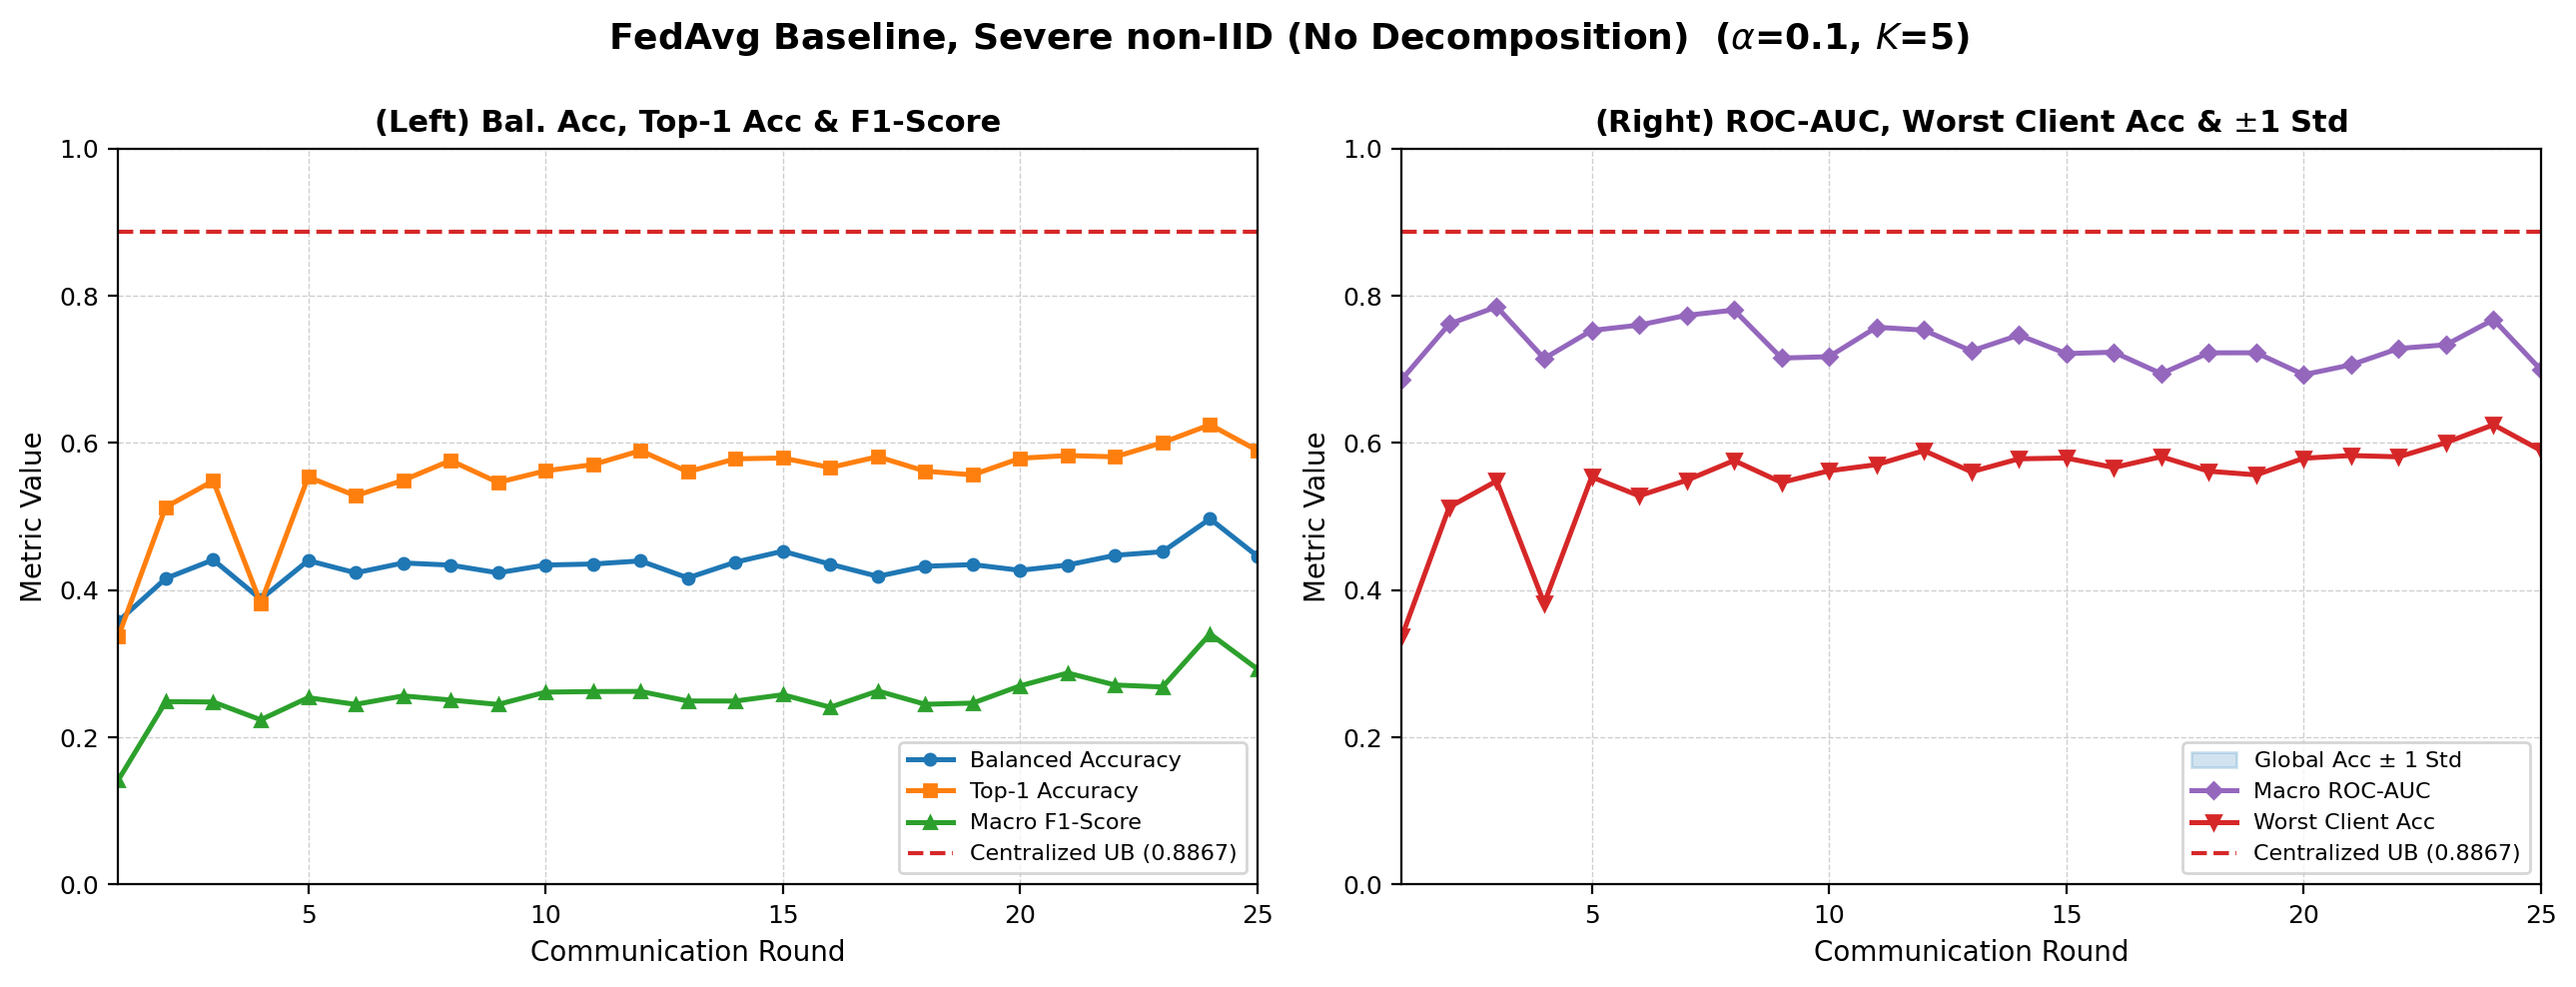
\includegraphics[width=0.80\textwidth]{images/fedavg_severe_curves.png}\\[4pt]
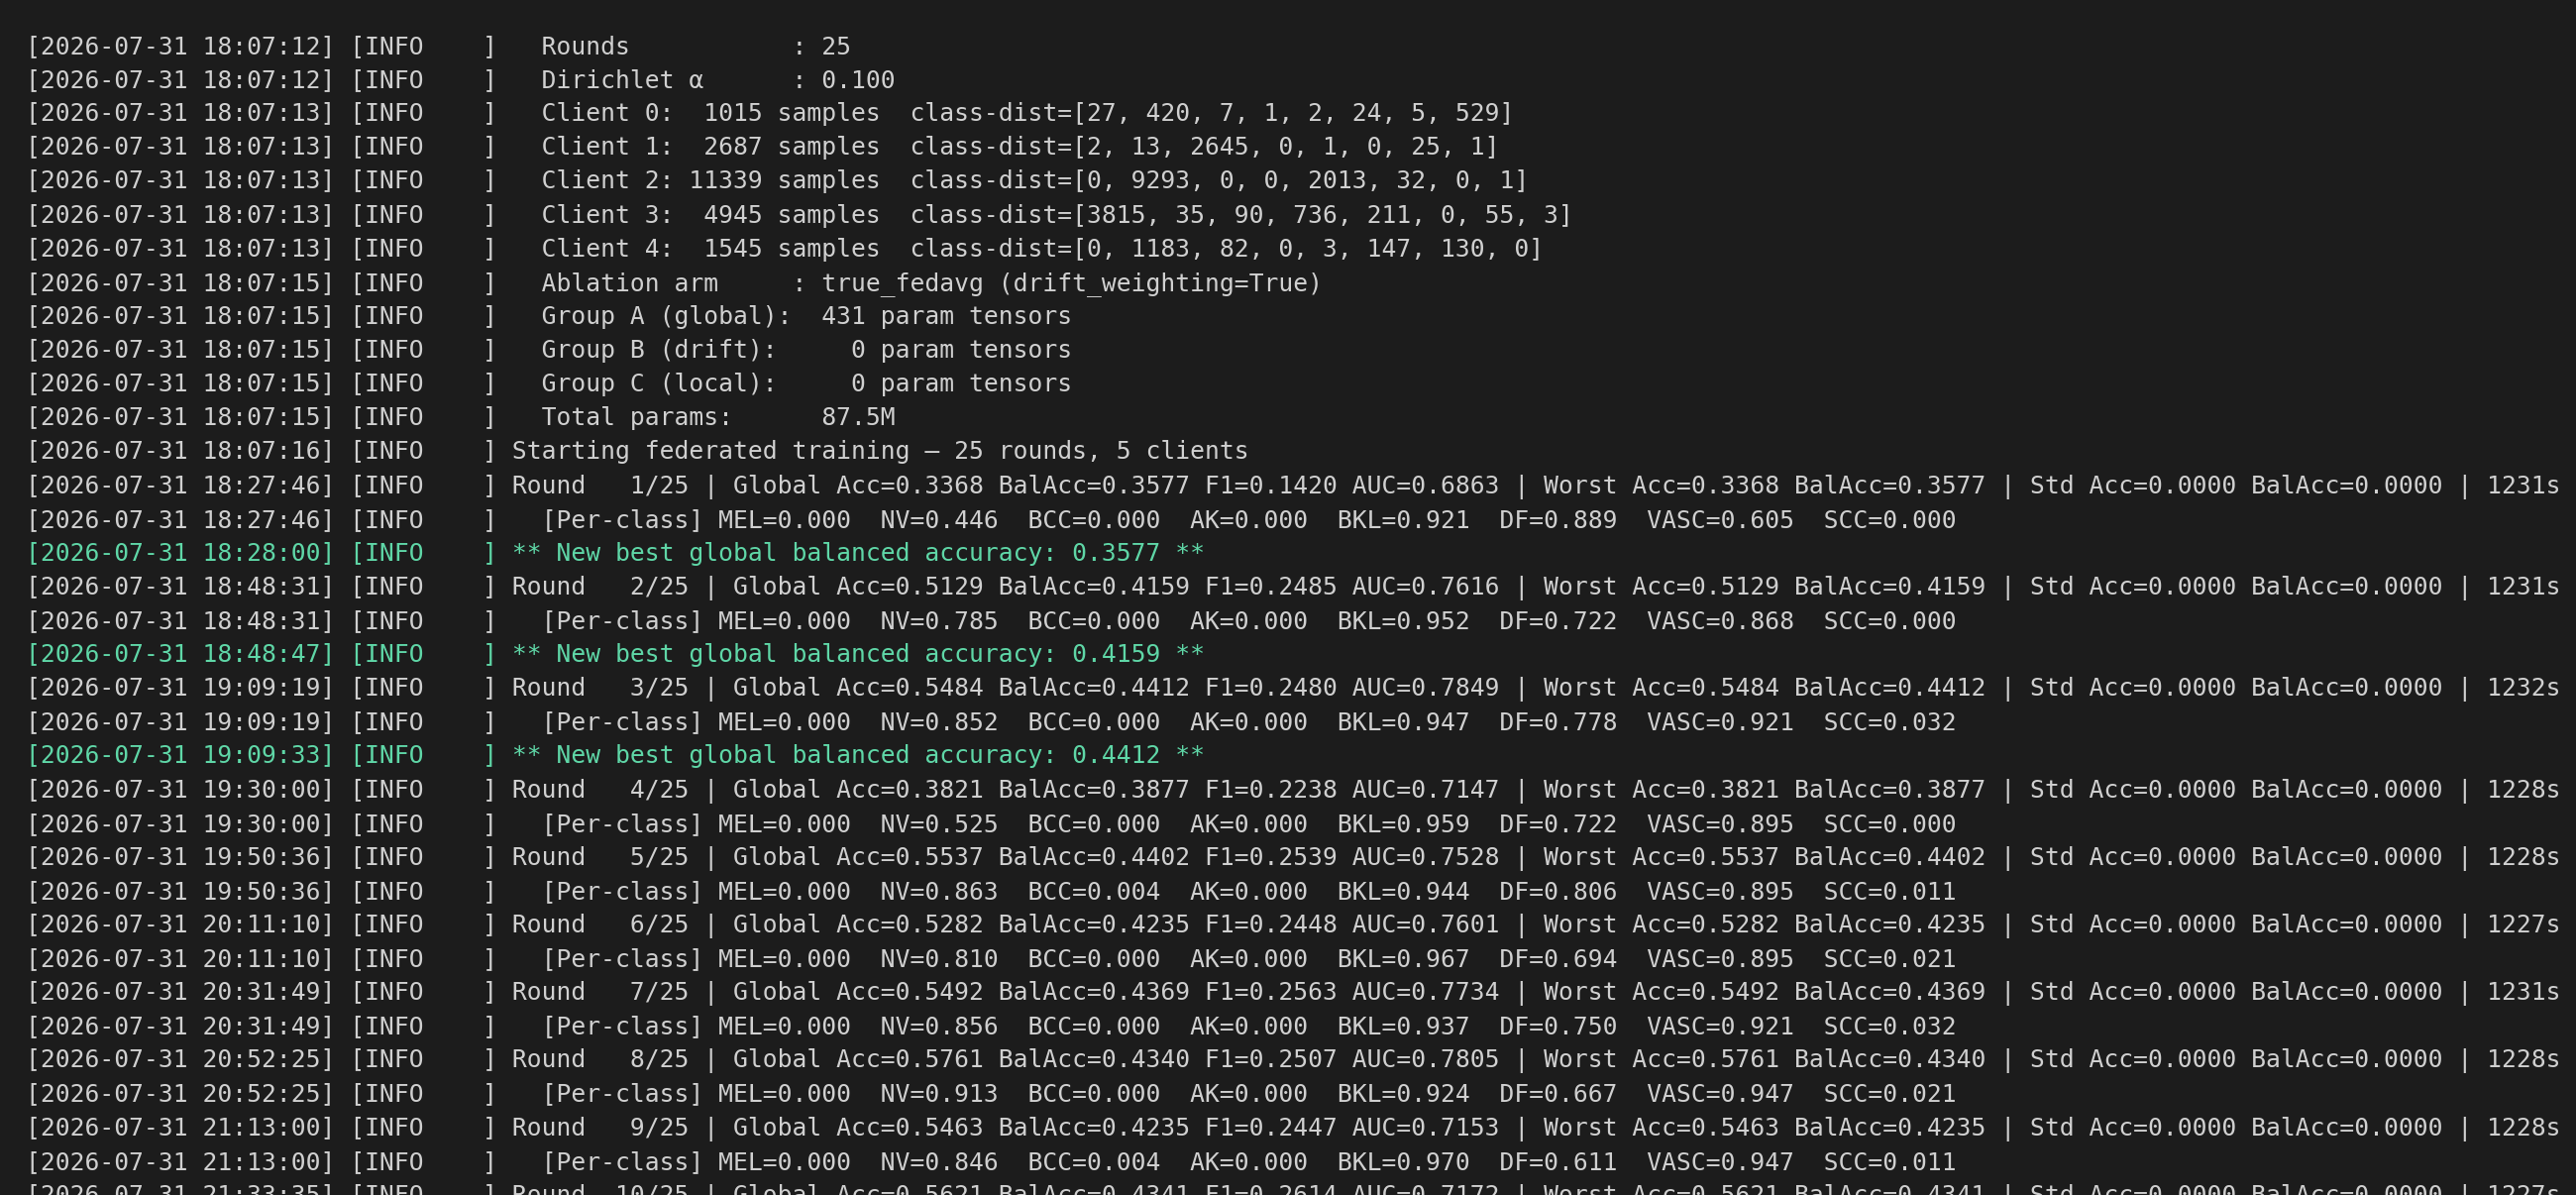
\includegraphics[width=0.80\textwidth]{images/fedavg_severe_terminal_top.png}\\[4pt]
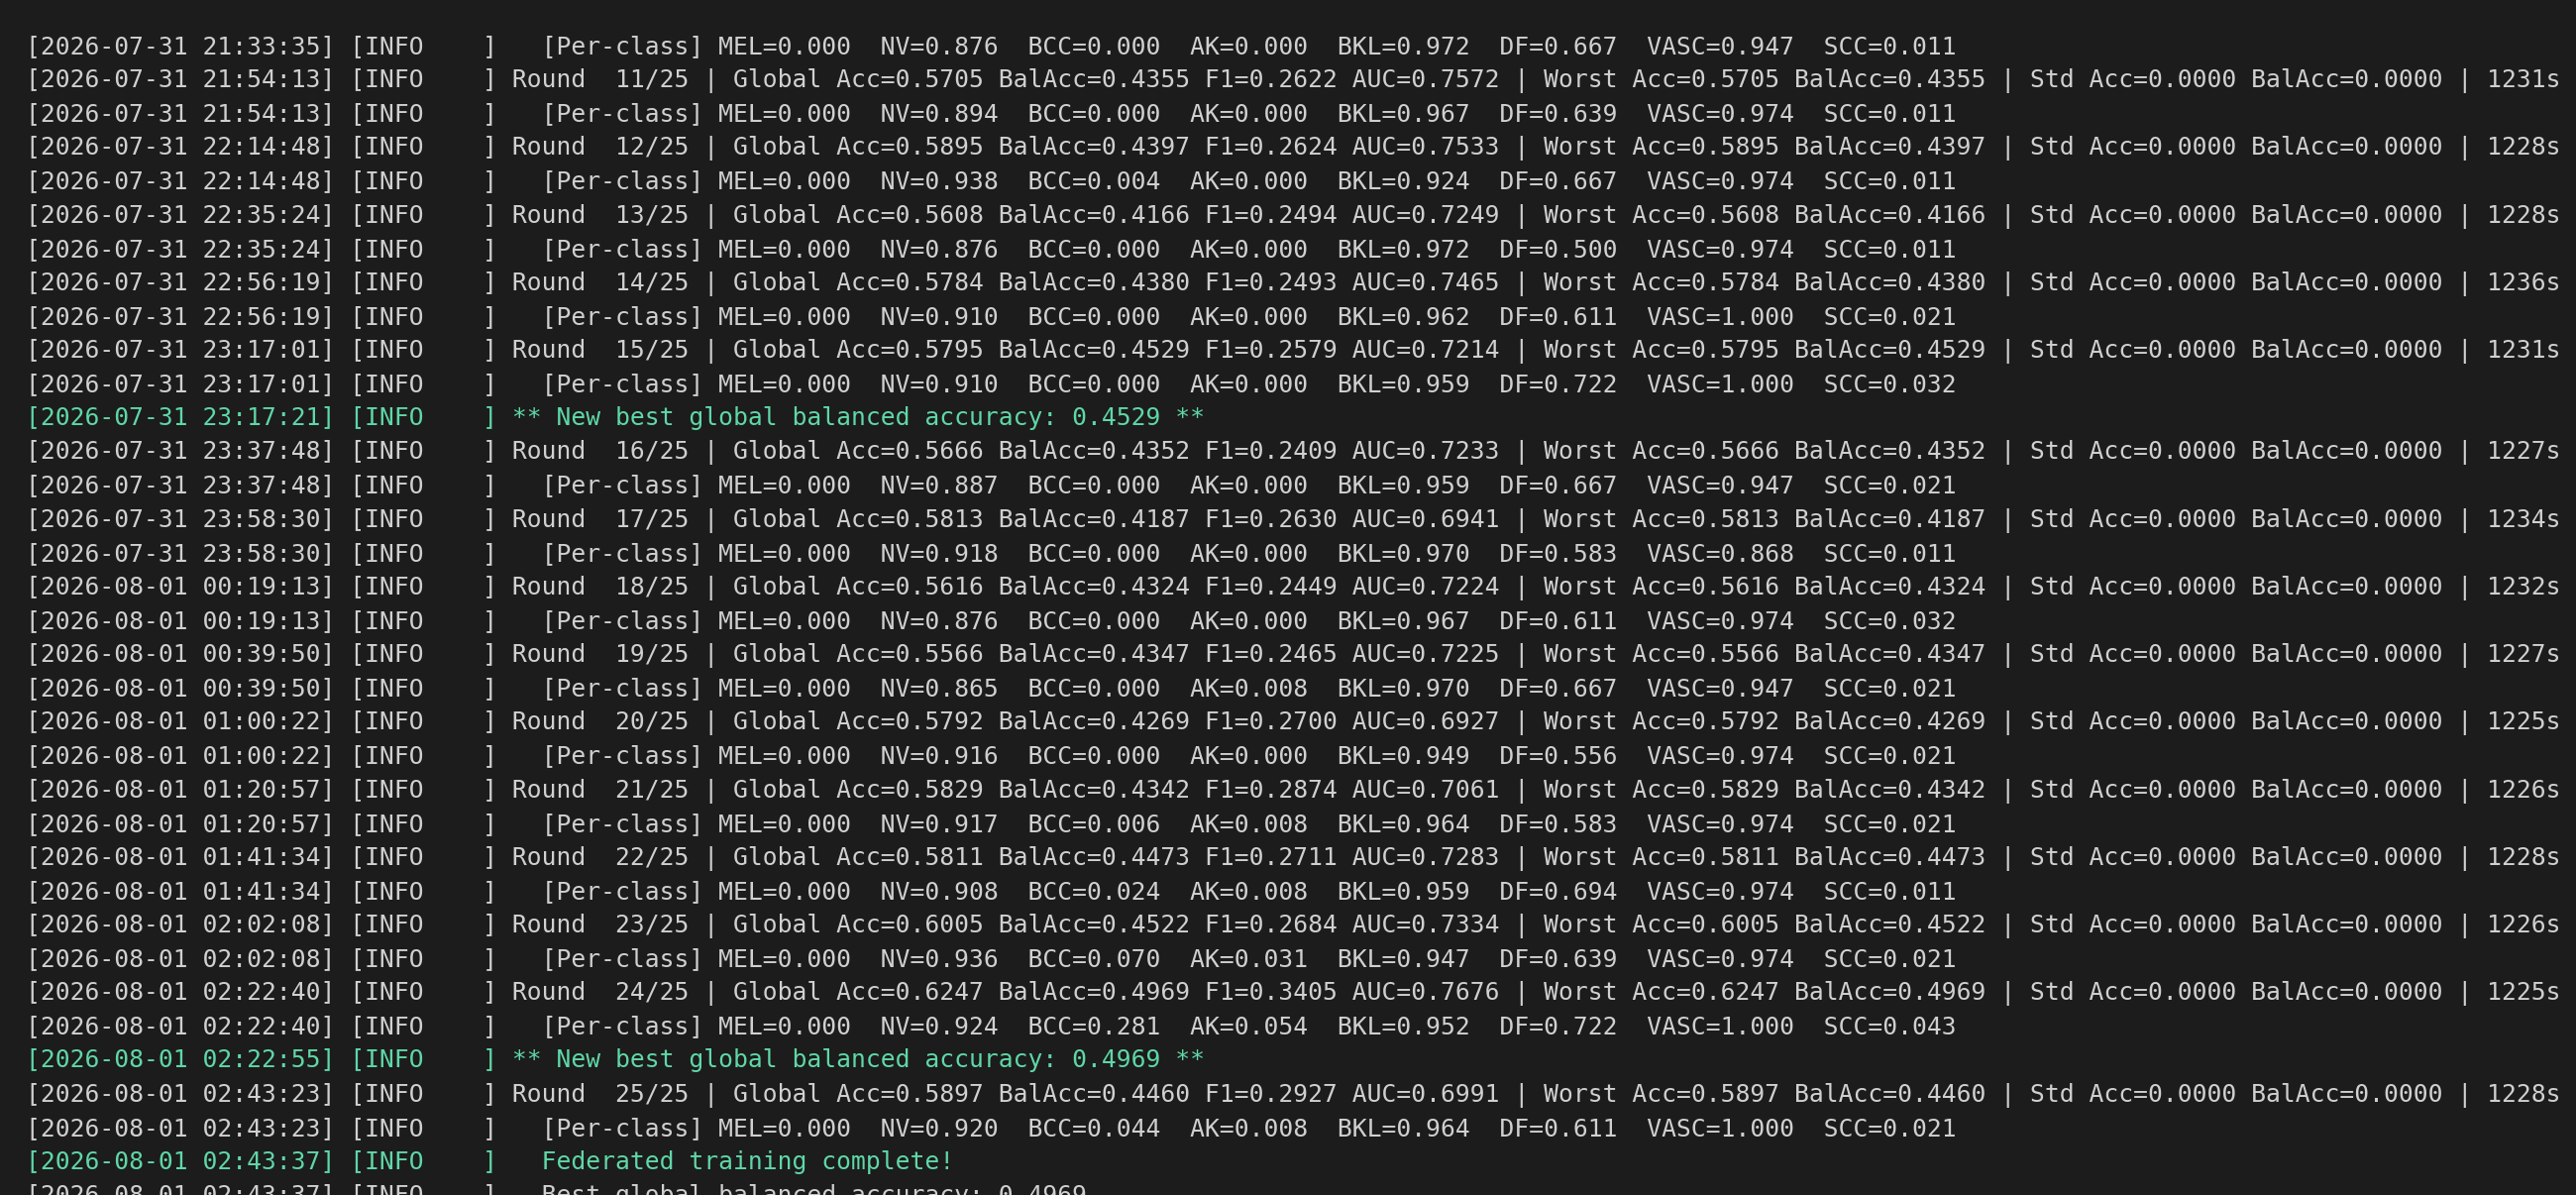
\includegraphics[width=0.80\textwidth]{images/fedavg_severe_terminal_bottom.png}
\caption[FedAvg severe non-IID (alpha=0.1, K=5)]{FedAvg baseline with the decomposition removed ($\alpha{=}0.1$, $K{=}5$): top panel shows convergence metrics; middle and bottom panels show terminal outputs. The per-class lines record \texttt{MEL=0.000} at every one of the 25 rounds, with \texttt{BCC}, \texttt{AK} and \texttt{SCC} at or near zero: the run reaches the highest overall accuracy of the three configurations while never predicting melanoma. Inter-client standard deviation is identically zero because no client-specific head exists. The \texttt{Ablation arm} line reports \texttt{drift\_weighting=True} because the command-line flag retains its default; with Group~B empty (0 tensors, shown two lines below) the drift rule has no parameters to act on and is inert, so this configuration is standard FedAvg.}
\label{fig:severe_fedavg_bundle}
\end{figure*}

\begin{figure*}[!t]
\centering
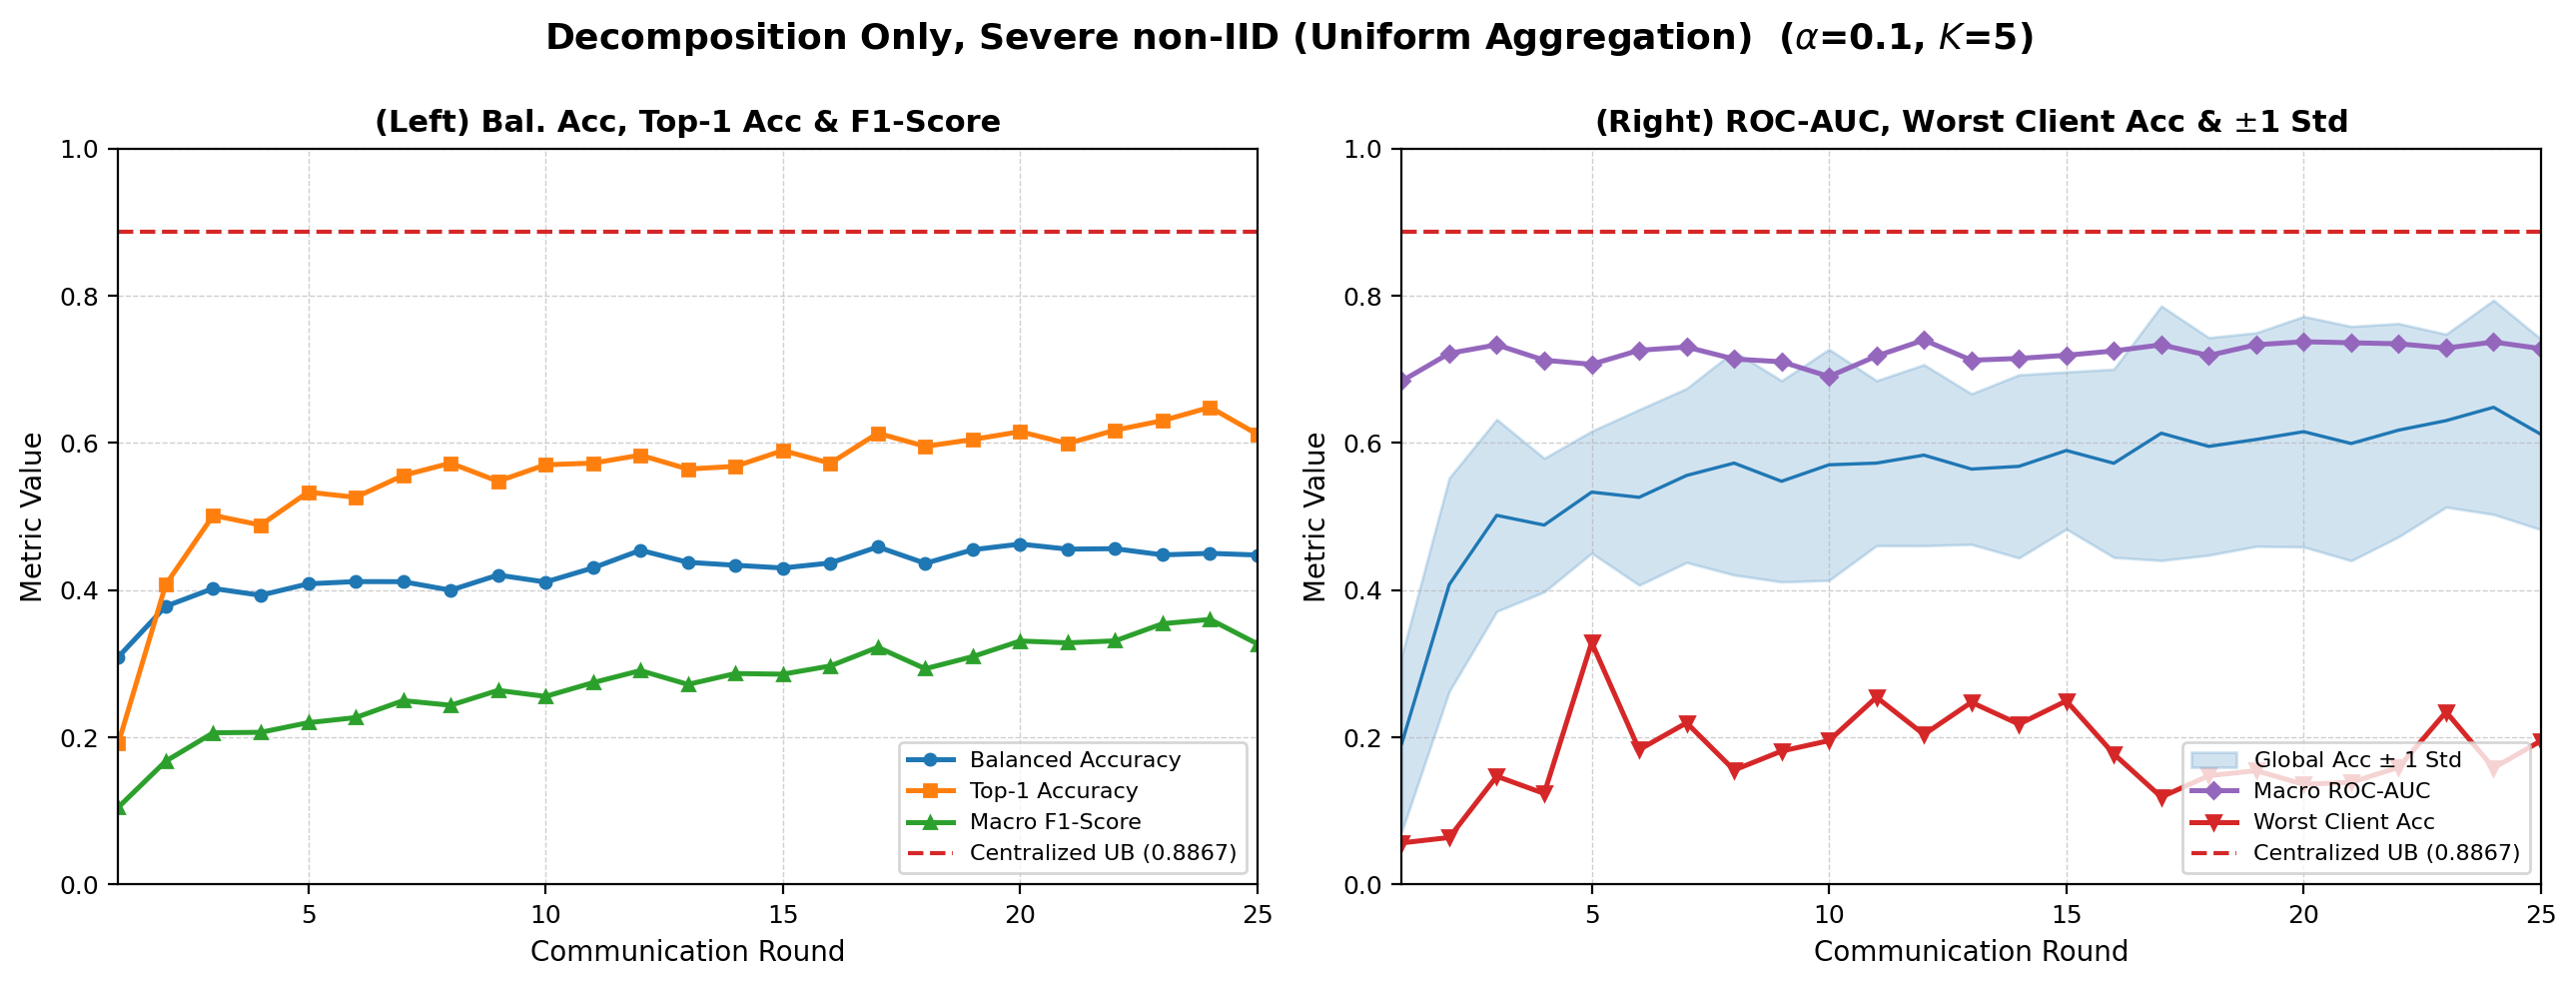
\includegraphics[width=0.80\textwidth]{images/decomp_only_severe_curves.png}\\[4pt]
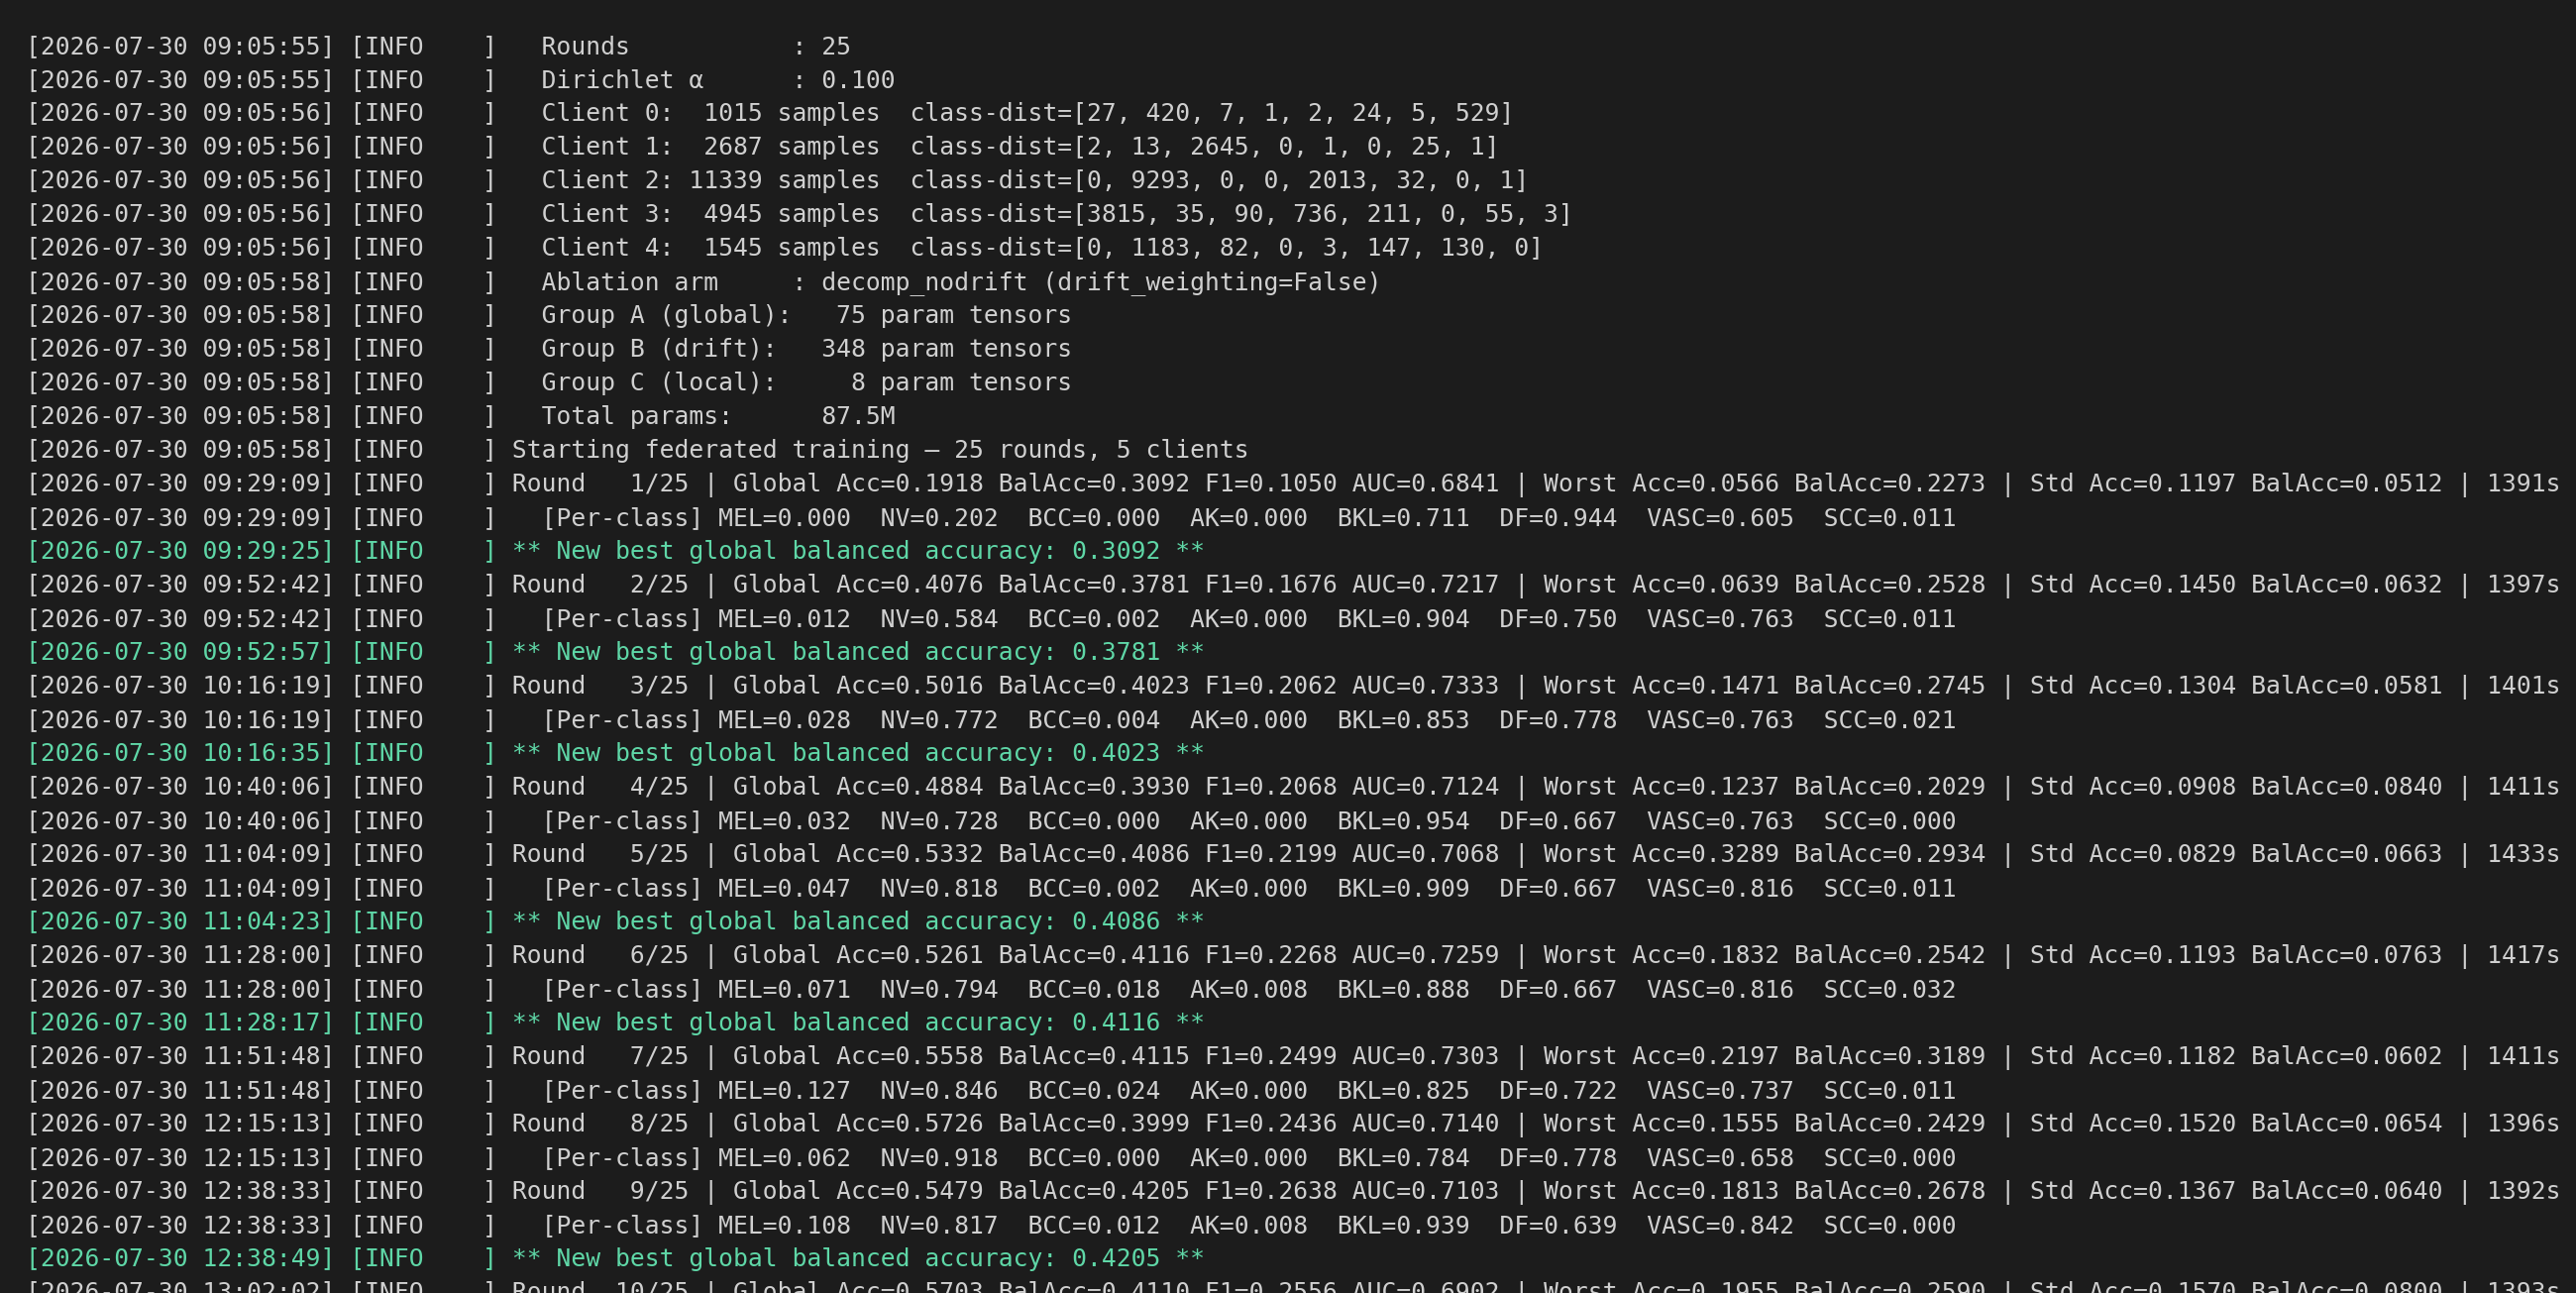
\includegraphics[width=0.80\textwidth]{images/decomp_only_severe_terminal_top.png}\\[4pt]
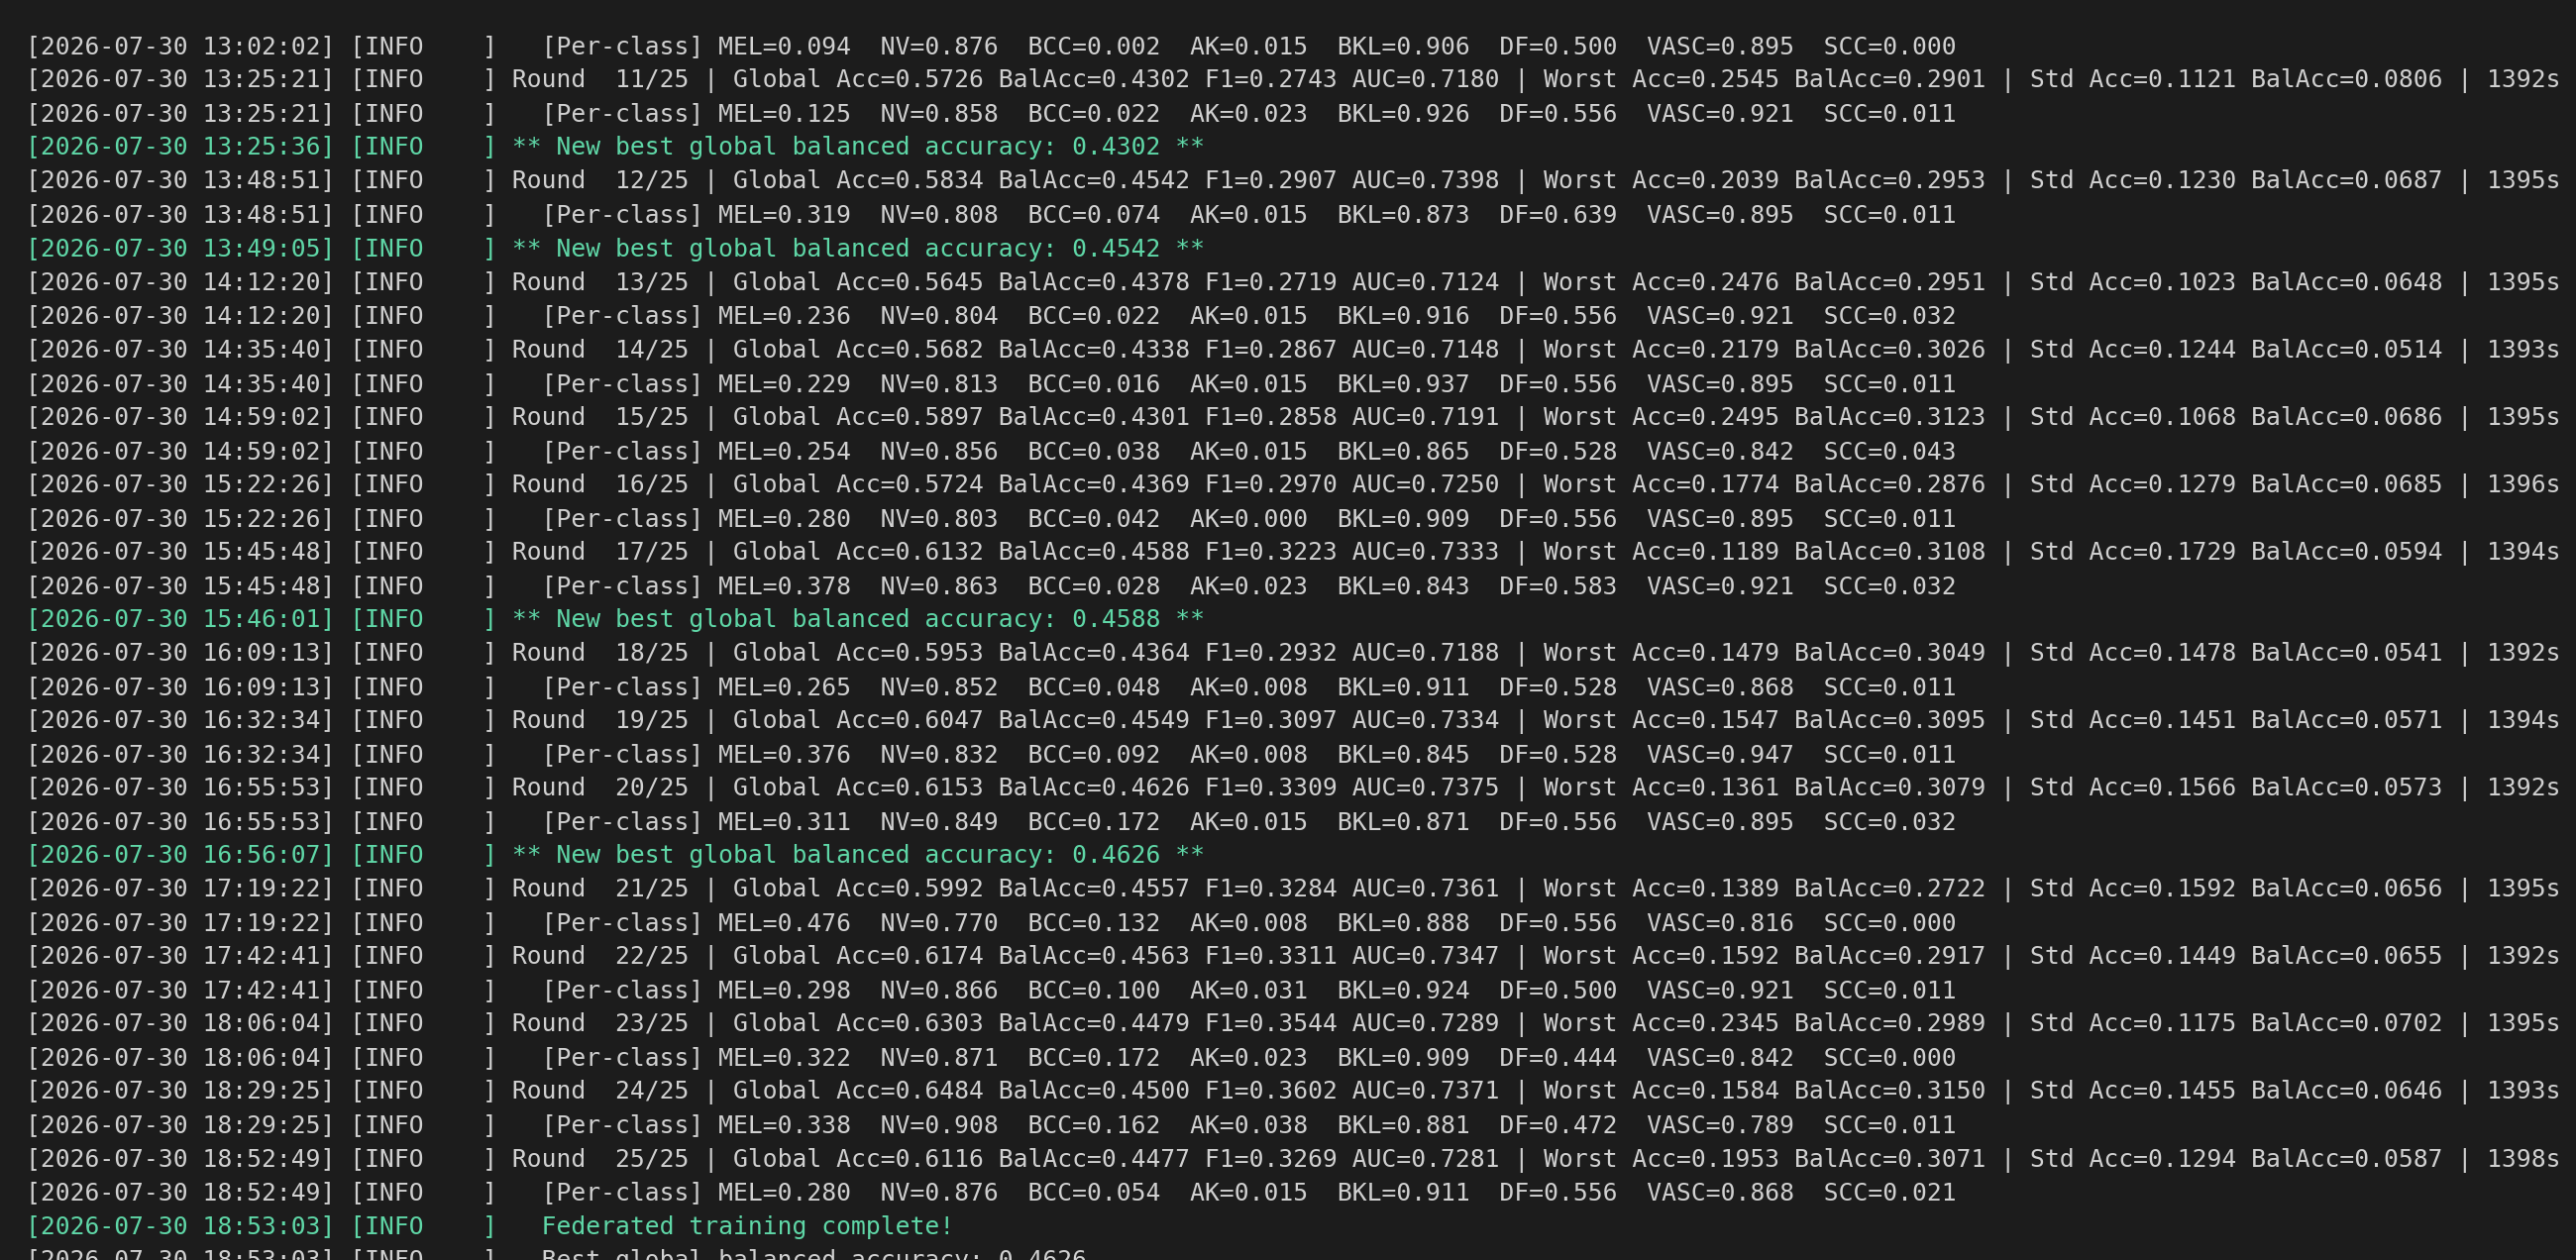
\includegraphics[width=0.80\textwidth]{images/decomp_only_severe_terminal_bottom.png}
\caption[Decomposition only, severe non-IID (alpha=0.1, K=5)]{Decomposition-only setting ($\alpha{=}0.1$, $K{=}5$, drift weighting disabled): top panel shows convergence metrics; middle and bottom panels show terminal outputs. All eight classes retain non-zero recall, but the worst-client floor is low and inter-client dispersion is wide. Final Balanced Accuracy: 0.4477, Worst Client Accuracy: 0.1953, standard deviation 0.1294.}
\label{fig:severe_decomp_bundle}
\end{figure*}

\begin{figure*}[!t]
\centering
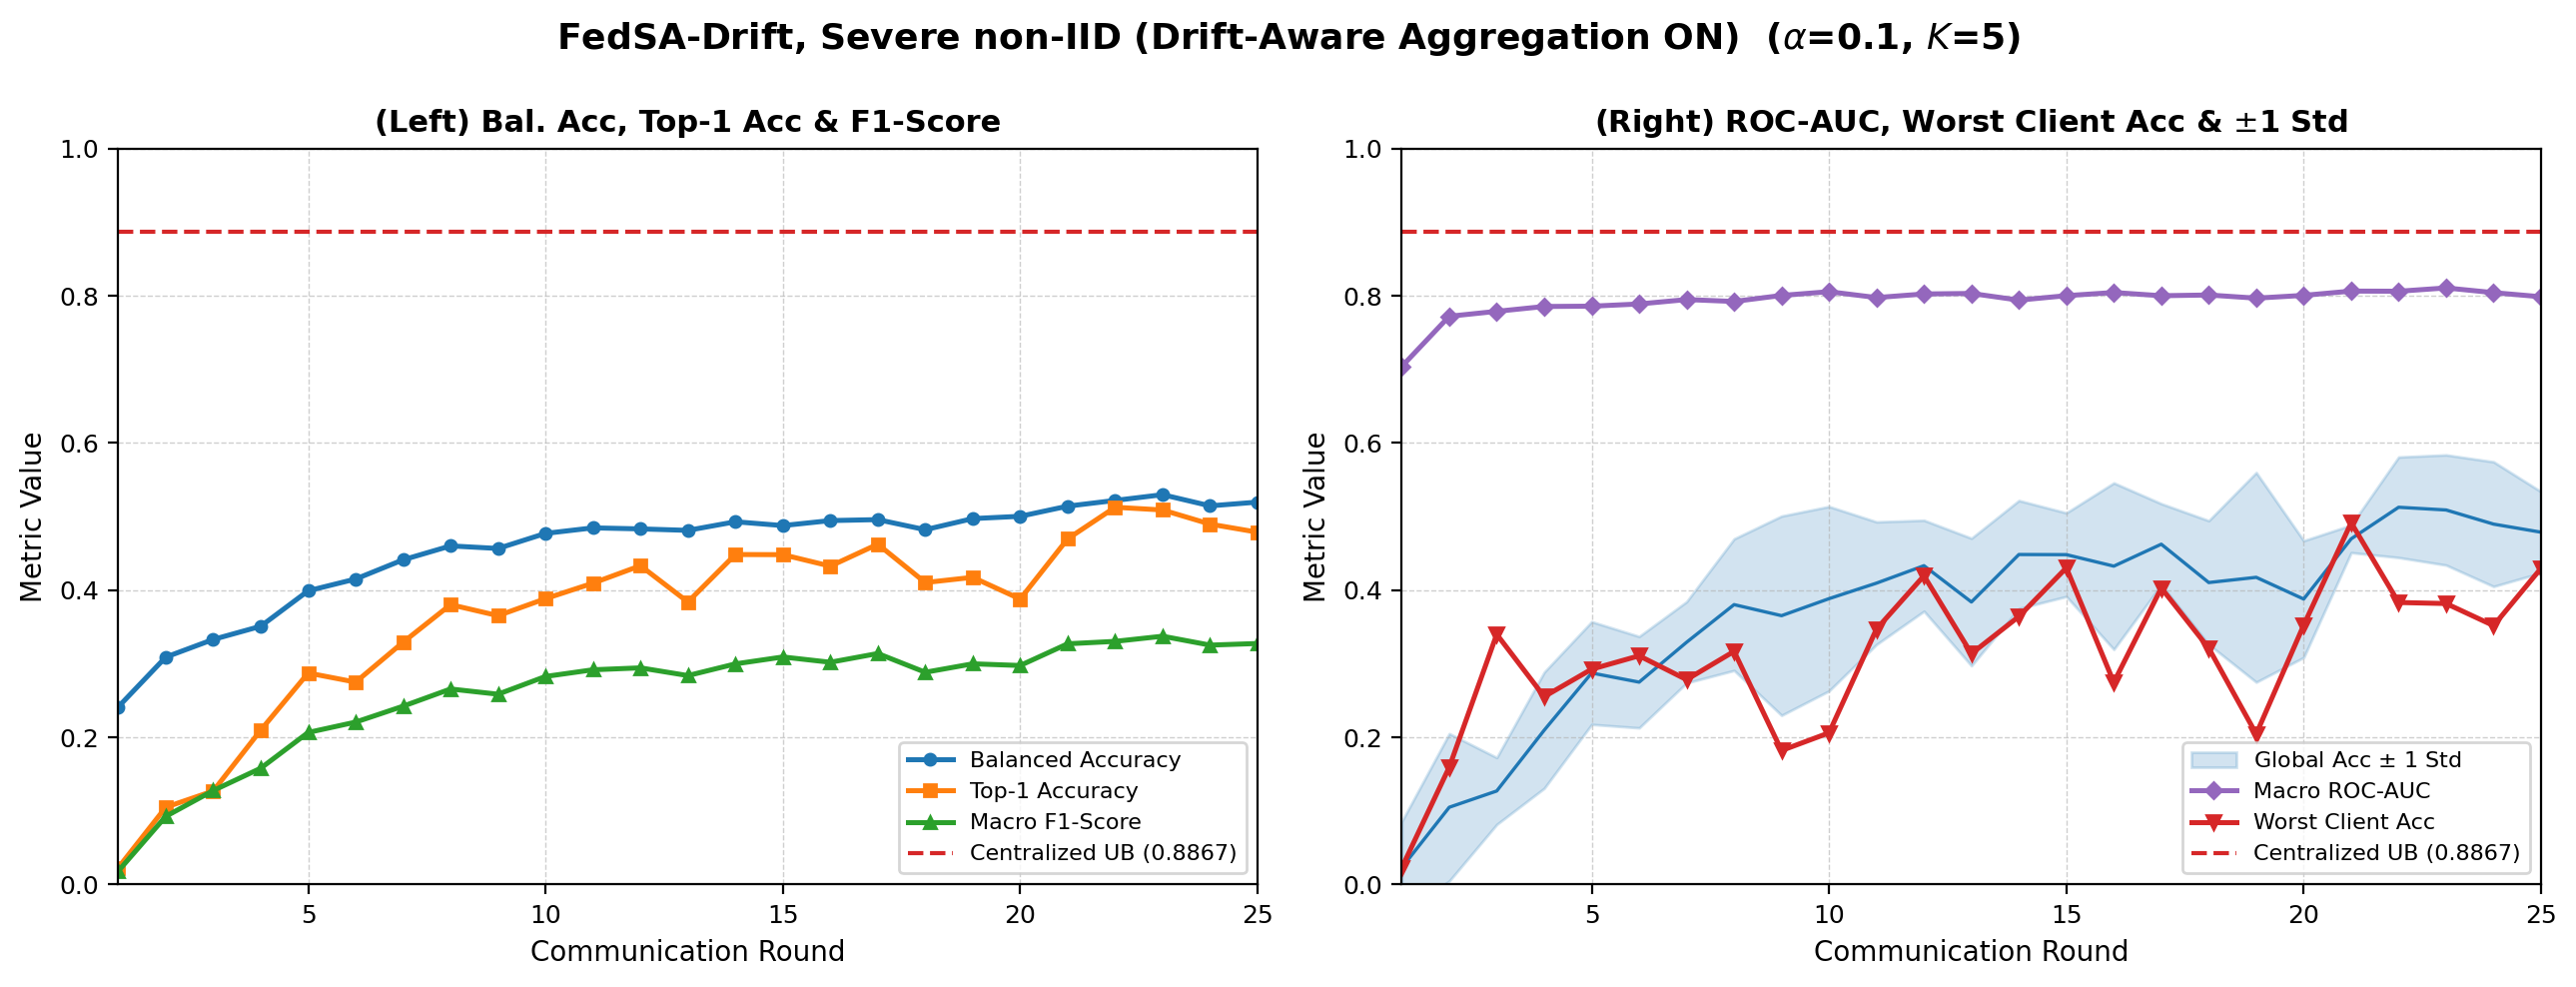
\includegraphics[width=0.80\textwidth]{images/sa_drift_severe_curves.png}\\[4pt]
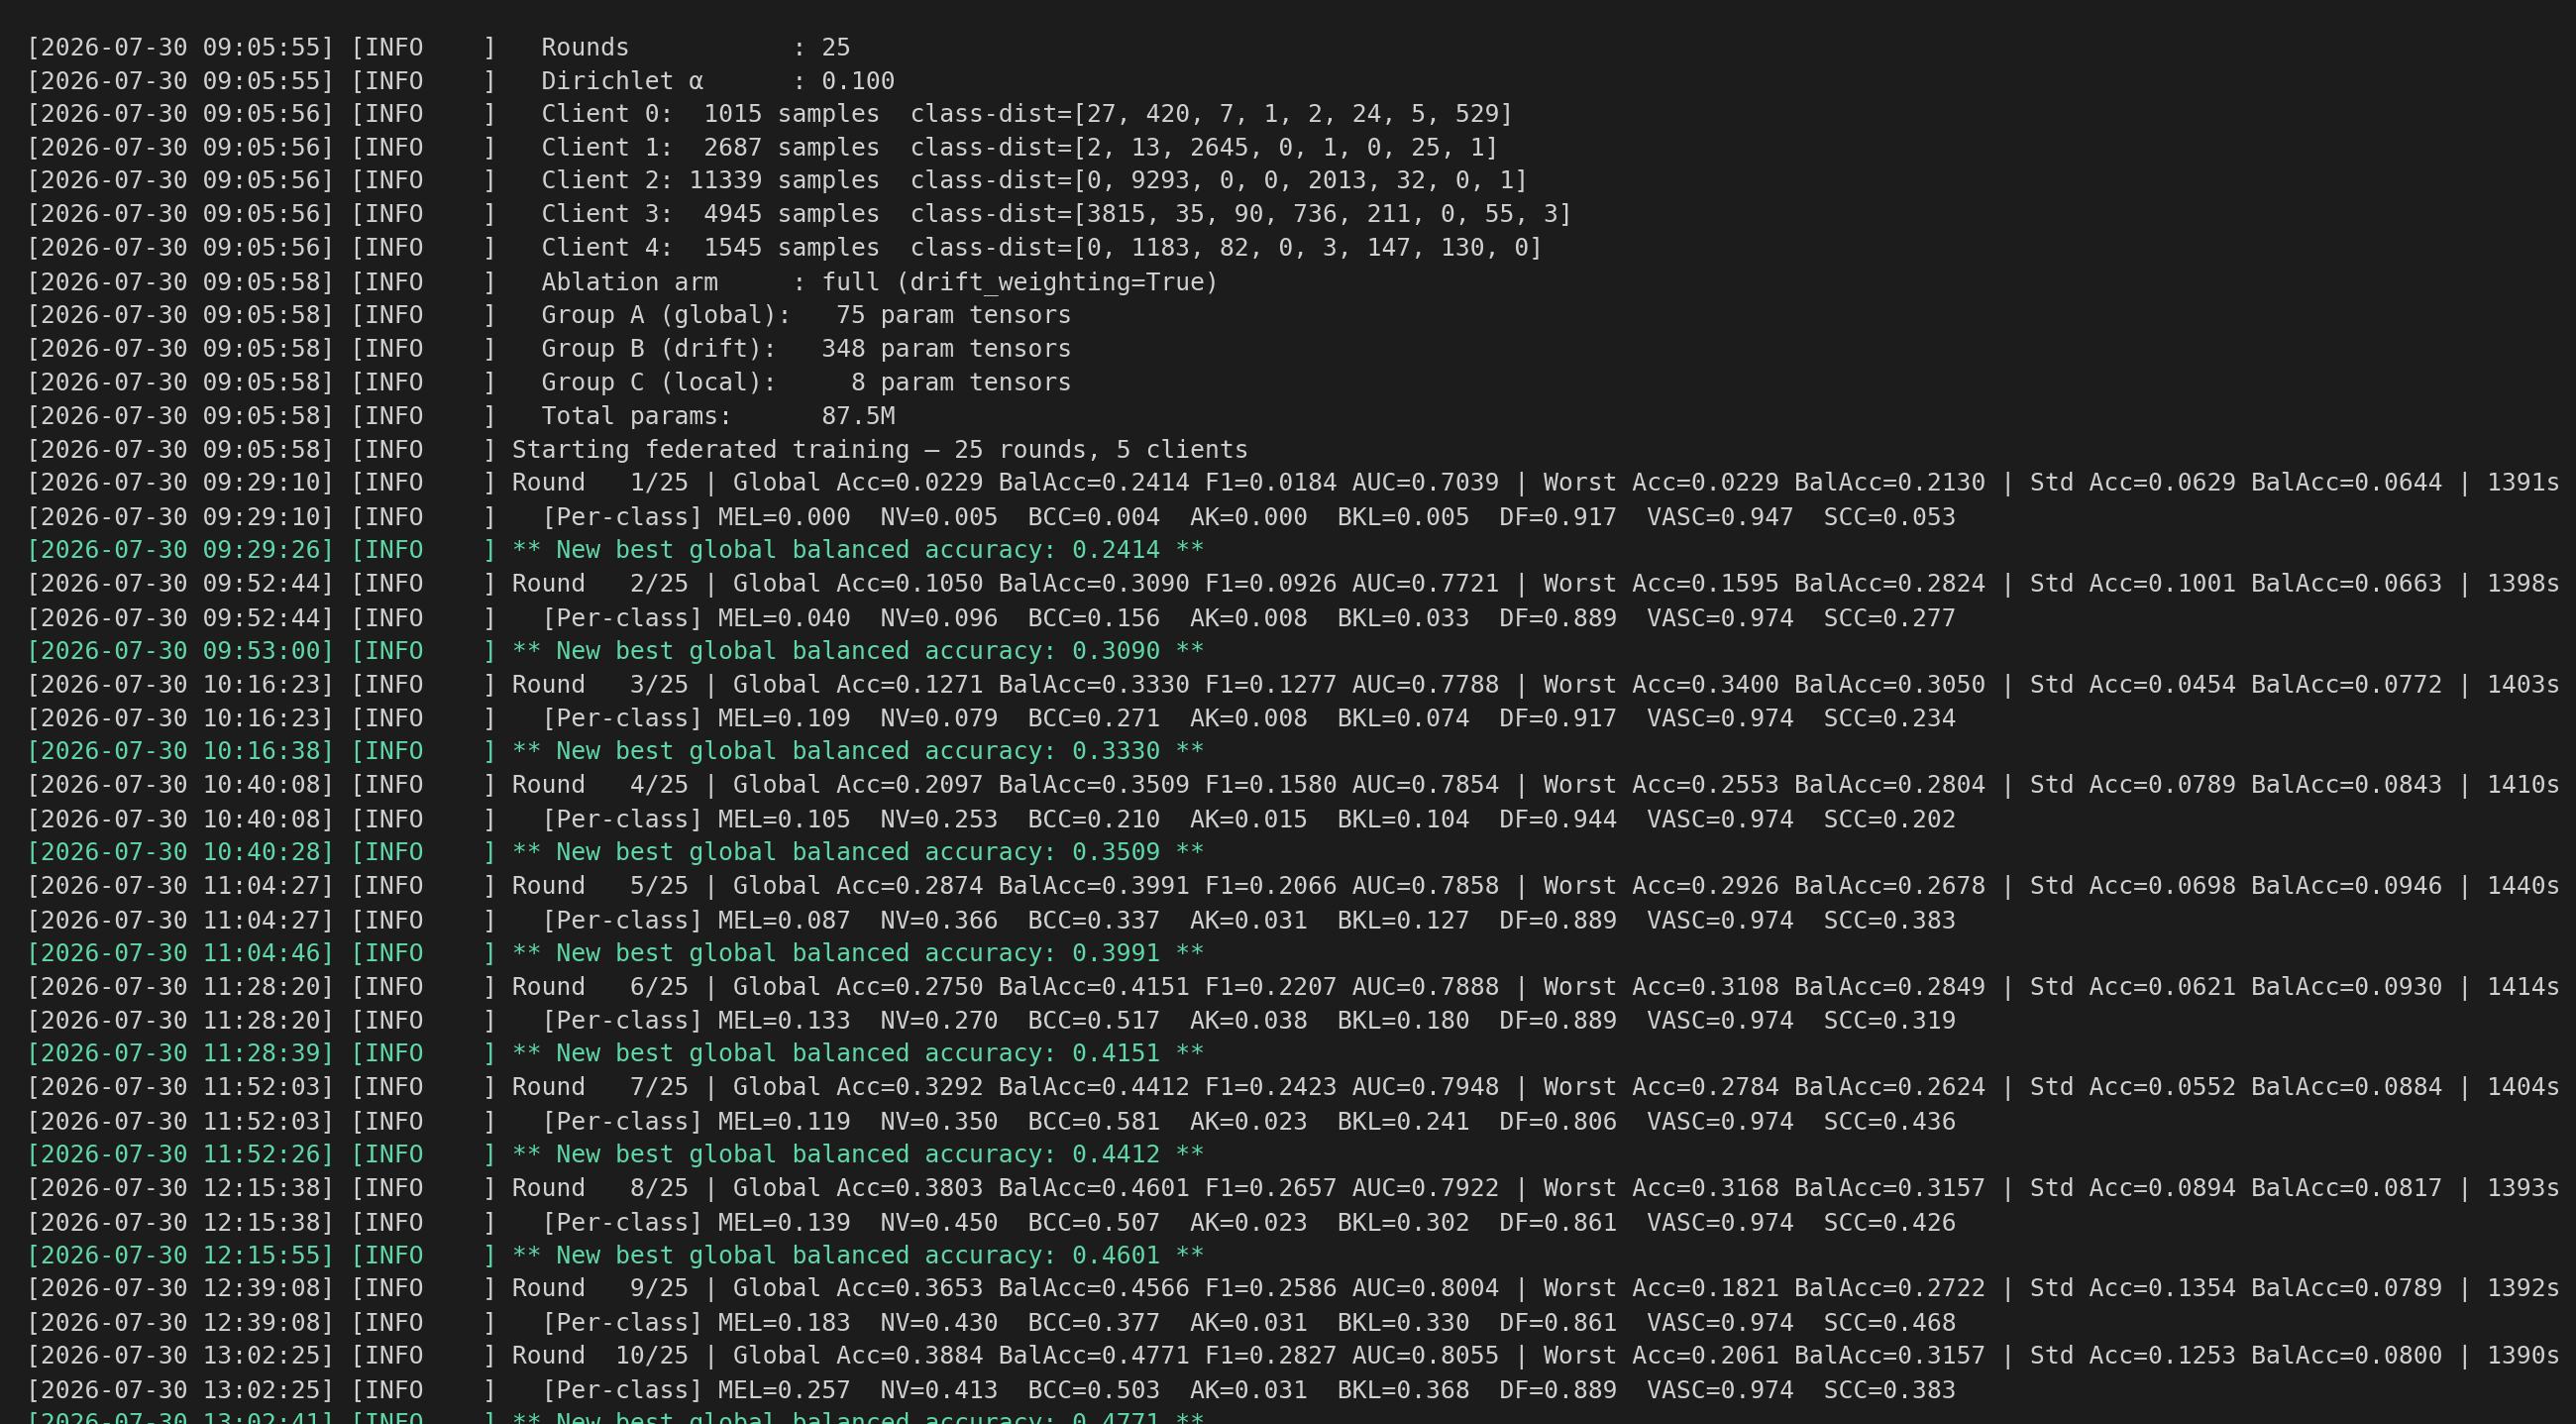
\includegraphics[width=0.80\textwidth]{images/sa_drift_severe_terminal_top.png}\\[4pt]
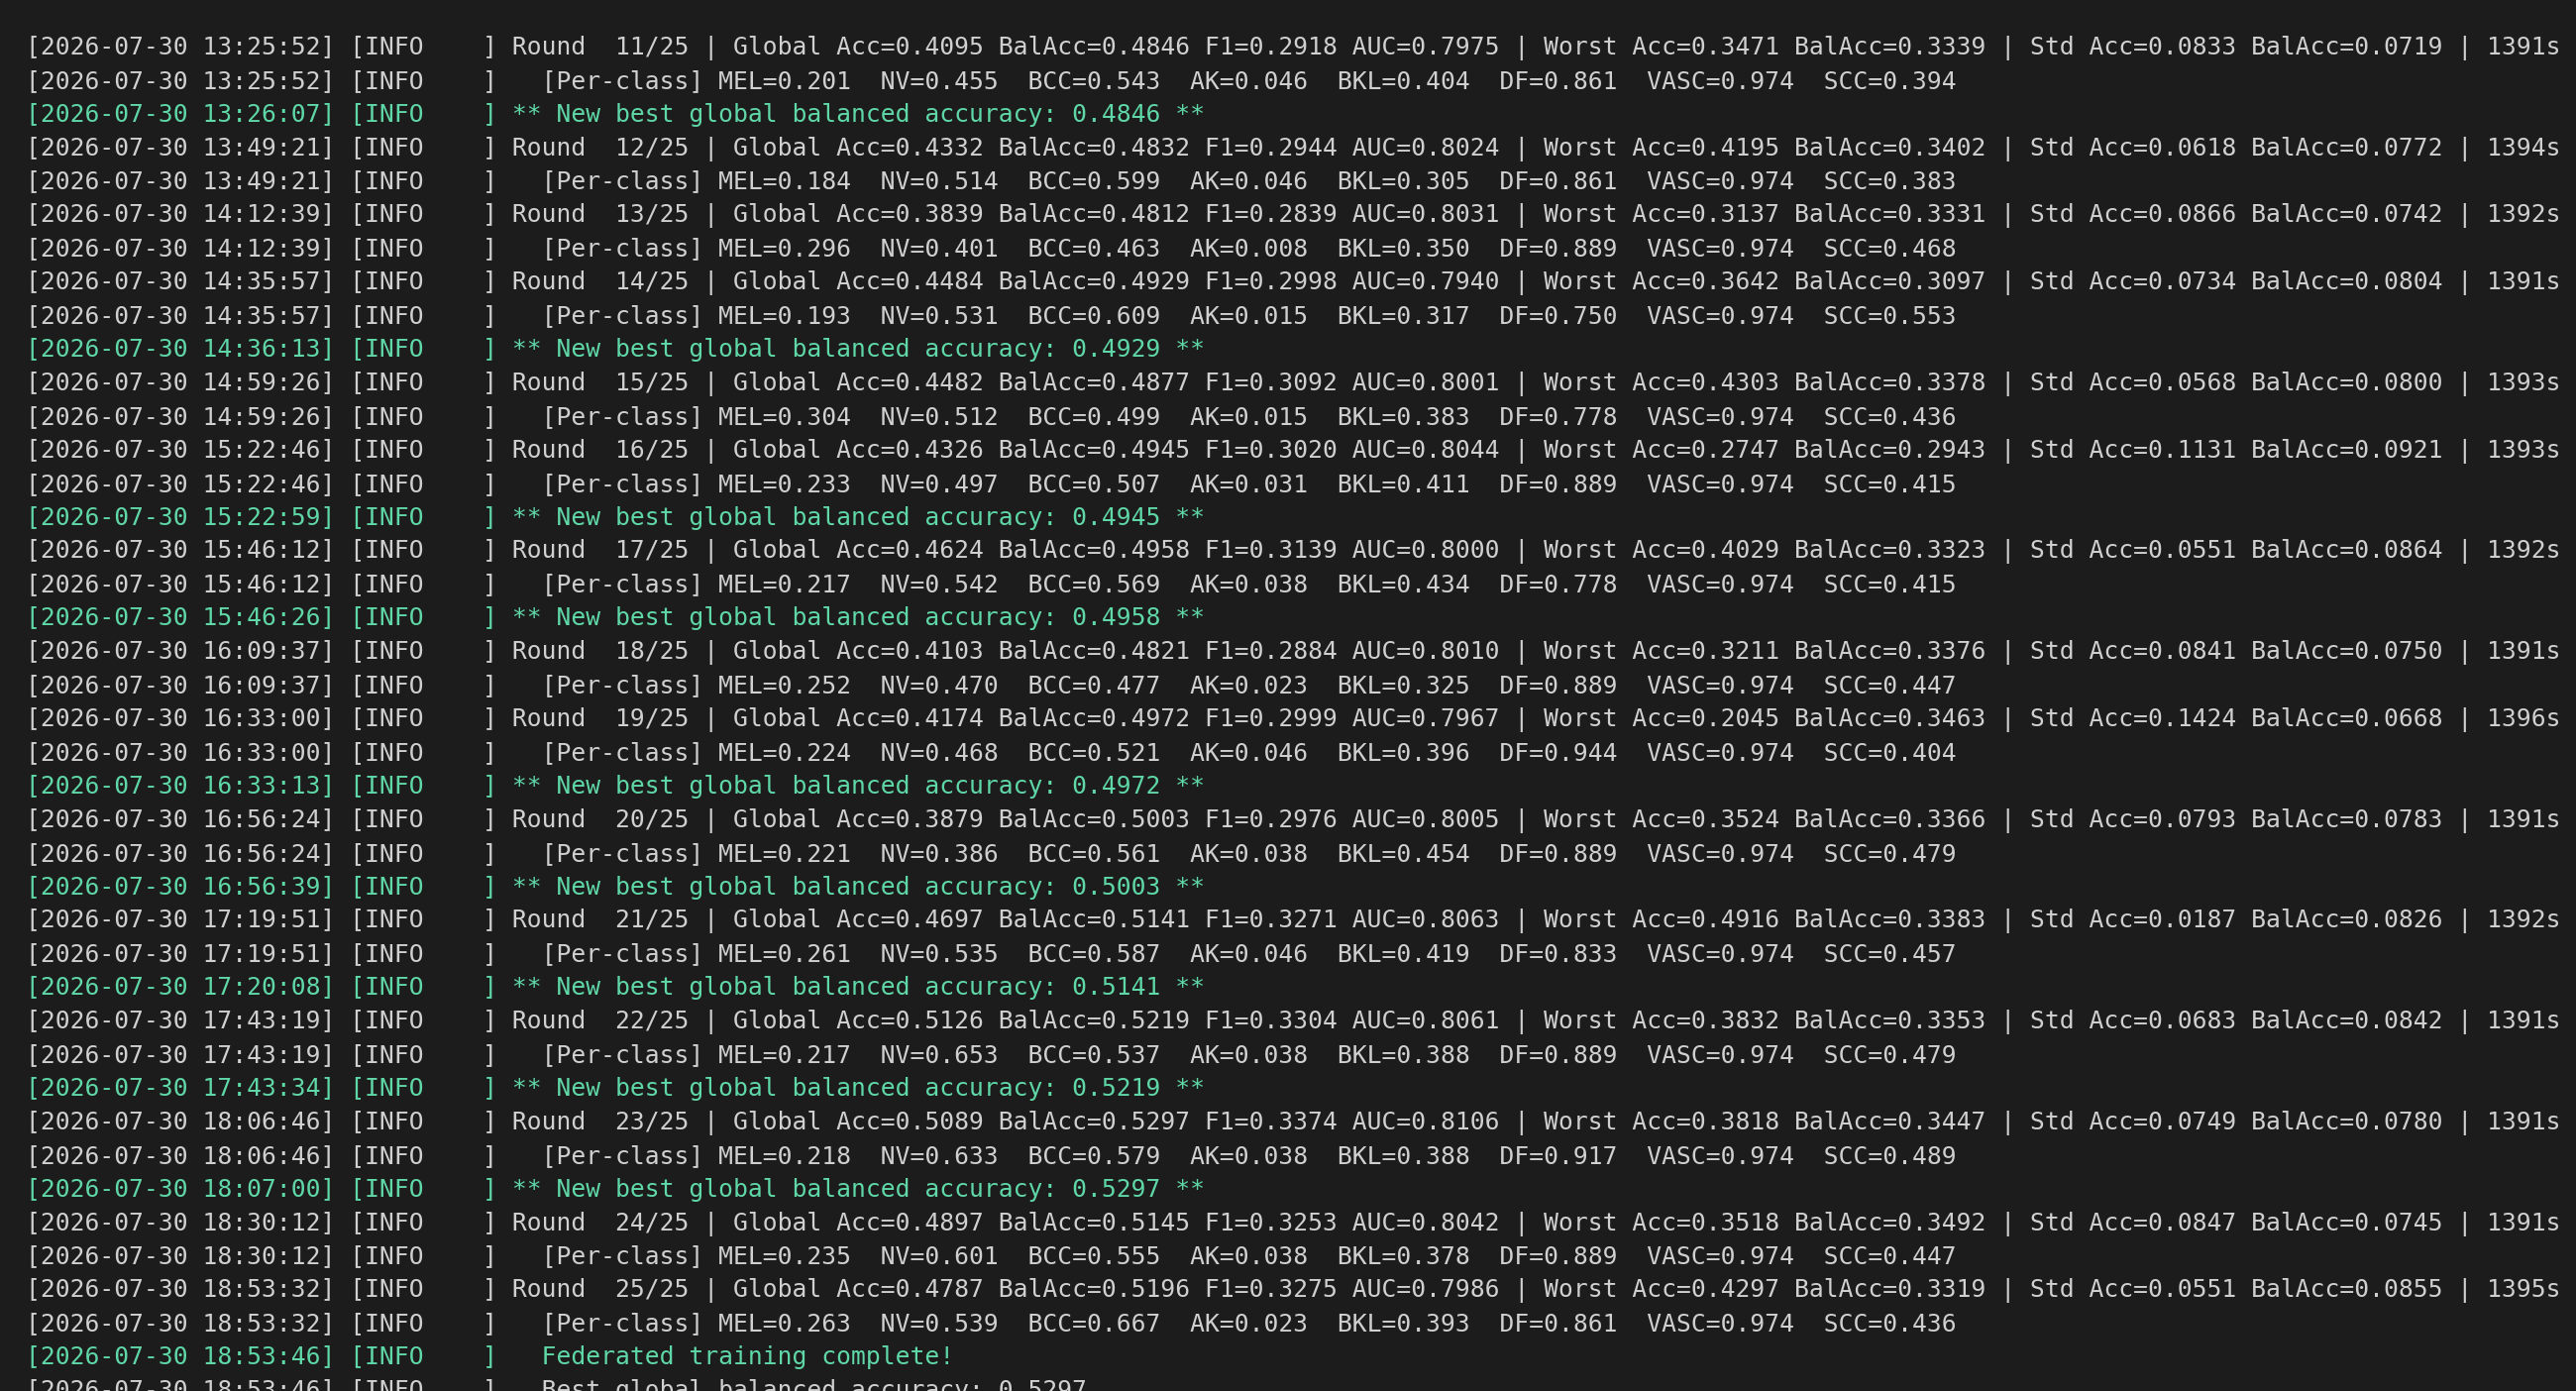
\includegraphics[width=0.80\textwidth]{images/sa_drift_severe_terminal_bottom.png}
\caption[FedSA-Drift severe non-IID (alpha=0.1, K=5)]{\sadrift{} severe non-IID setting ($\alpha{=}0.1$, $K{=}5$): top panel shows convergence metrics; middle and bottom panels show terminal outputs. Final Balanced Accuracy: 0.5196, Worst Client Accuracy: 0.4297, inter-client standard deviation 0.0551. All eight classes retain non-zero recall throughout.}
\label{fig:severe_sadrift_bundle}
\end{figure*}

\subsubsection{Interpreting the Global Accuracy Trade-off}

\sadrift{} achieves a lower global balanced accuracy than the uniform-aggregation baseline at the milder settings (0.8209 vs.\ 0.8314 at $\alpha{=}1.0$; 0.7066 vs.\ 0.7622 at $\alpha{=}0.5$). The more pronounced gap at $\alpha{=}0.5$ (5.6 percentage points, vs.\ 1.1 at $\alpha{=}1.0$) reflects a genuine cost of the fairness--utility trade-off that is well-recognized in the federated learning literature~\cite{Li2021,Mohri2019}. We do not claim this cost is negligible; a global accuracy reduction of this magnitude in medical imaging warrants careful clinical evaluation before deployment.

The relevant comparison, however, is not global accuracy in isolation. Under FedAvg at $\alpha{=}0.5$, the worst-performing client reaches only 48.0\% balanced accuracy---little better than chance for an eight-class problem. \sadrift{} raises this floor to 57.1\%. The minimax fairness objective~\cite{Mohri2019,Li2021}, which optimizes the worst-case client rather than the population average, has been explicitly motivated in federated healthcare AI contexts where a model that fails disproportionately at one institution creates inequities in clinical outcomes~\cite{Darzi2024,Rieke2020}. Improving the minimum performance guarantee at the cost of some global average is the stated design goal of \sadrift{}, and the observed trade-off is consistent with that goal. A comprehensive clinical validation comparing deployment outcomes across institutions is an important direction for future work.

The direction of this trade-off is not fixed. At $\alpha{=}0.1$ it reverses within the decomposed family: \sadrift{} attains \emph{higher} global balanced accuracy than decomposition alone (0.5196 vs.\ 0.4477), so drift-aware weighting costs nothing in aggregate utility once heterogeneity is severe, while still raising the worst-client floor by 23.4 points. The utility cost seen at $\alpha \in \{0.5, 1.0\}$ therefore appears to be a feature of mild heterogeneity rather than an inherent price of the method.

A separate comparison applies once the decomposition itself is removed. The no-decomposition FedAvg baseline at $\alpha{=}0.1$ records the highest mean per-client accuracy of the three configurations (0.4702 on the held-out test split, against 0.4264 for \sadrift{}), and marginally higher balanced accuracy (0.3778 vs.\ 0.3681). We do not present \sadrift{} as superior on aggregate accuracy in this regime. As Section~\ref{sec:threeway} shows, that baseline reaches its figure by abandoning four of the eight diagnostic classes outright, so the aggregate comparison and the clinical comparison point in opposite directions.

\subsection{Contextual Reference Against Related Methods}
\label{sec:sota_comparison}

Table~\ref{tab:sota_comparison} places \sadrift{} alongside related published methods for contextual reference. \textbf{This is not a controlled head-to-head comparison.} The methods listed use different backbone architectures, training datasets, class distributions, federation setups, and evaluation protocols; direct numerical comparison is therefore not appropriate. The table is intended only to situate the design choices and claims of \sadrift{} within the broader literature.

\begin{table*}[t]
\centering
\caption{Contextual Reference Comparison with Related Methods. \textbf{Note:} methods differ in dataset, backbone, class count, and experimental setup. Direct numerical comparison is inappropriate; this table contextualizes design choices only.}
\label{tab:sota_comparison}
\begin{tabular}{p{2.8cm}p{2.4cm}p{2.2cm}p{2.0cm}p{3.2cm}p{2.8cm}}
\toprule
Method & Backbone & Multimodal & Dataset & Key Performance & Client Overhead \\
\midrule
MedFusionNet~\cite{Naeem2025} & ConvNeXt + ViT-B16 & No (images) & ISIC 2019 / HAM & Acc: 97.5--98.0\% (Cent.) & N/A (Centralized) \\
FedMHA~\cite{Darzi2024} & Pre-trained ViT & No (images) & ISIC (LDA $\alpha \in [0.1, 0.9]$) & Acc: 67.09\% ($\alpha{=}0.1$) to 83.99\% ($\alpha{=}0.9$) & High (matrix distance) \\
FedAPM~\cite{Zhu2025} & CNN / MLP & Yes (partial pers.) & CIFAR / Multimodal & Top across pFedMe/DITTO baselines & Very high (ADMM) \\
EFTViT~\cite{Wu2024} & Vision Transformer & No (images) & CIFAR / ISIC (sim.) & GFLOPs reduced by up to 5.6$\times$ & Low (75\% patch mask) \\
DAFL~\cite{Zhao2025} & ViT / CNN & No (images) & Medical (non-IID) & Adaptive focal reweighting & Medium (local focal tuning) \\
Async-FL-CNN~\cite{Yaqoob2023} & Standard CNN & No (images) & ISIC 2019 & Prec: 96.7\% / Spec: 96.3\% & Medium (async updates) \\
\midrule
\textbf{\sadrift{} (Ours)} & \textbf{SwinV2-Base} & \textbf{Yes (metadata MLP)} & \textbf{ISIC 2019 (LDA $\alpha \in [0.1, 1.0]$)} & \textbf{Bal.\ Acc: 88.67\% (Cent., internal val.) / 82.09\% (Fed $\alpha{=}1.0$, shared model)} & \textbf{None (server-side $O(|\mathbf{w}|)$)} \\
\bottomrule
\end{tabular}
\end{table*}

\subsubsection{Comparison with Centralized Baselines}

We do not benchmark our centralized figure against published ISIC 2019 results. Ours is measured on an internal validation split that shares lesions with the training partition, whereas challenge results are computed on the official held-out test collection; the two are not comparable, and the comparison is omitted rather than qualified.

\subsubsection{Comparison with Federated Vision Transformers}

Under non-IID data, standard FedAvg with self-attention results in feature collapse due to misaligned attention matrices.

\textbf{FedMHA}~\cite{Darzi2024} penalizes Euclidean deviations in the attention matrices during local backpropagation. FedMHA achieves accuracy ranging from 67.09\% to 83.99\% on the ISIC dataset across $\alpha \in [0.1, 0.9]$, while incurring the overhead of aligning the attention matrices at every local training iteration. \sadrift{} instead aggregates Group~A with FedAvg and down-weights deep-layer drift at the server. We did not measure attention-matrix stability and make no claim about it; the comparison here is one of mechanism and cost, not of effect. There is no modification to the client-side objective function. \sadrift{} records 82.09\% balanced accuracy at $\alpha = 1.0$ against 83.99\% for FedMHA at $\alpha = 0.9$, but we caution against reading these as comparable. The figures differ in dataset split, backbone, client count and heterogeneity level, and ours is measured on our internal validation split rather than a shared benchmark. We draw no conclusion from the difference. \sadrift{} also supports the use of multimodal metadata, which FedMHA does not.

\textbf{EFTViT}~\cite{Wu2024} utilizes a masking methodology that removes 75\% of input patches to lower the number of FLOPs in processing an image. By doing so, it creates a break in the contiguous spatial windows of SwinV2, which subsequently breaks cross-window connectivity. In contrast, \sadrift{} maintains full spatial representations and achieves drift mitigation purely at the server with zero client-side cost.

\subsubsection{Comparison with Partially Personalized Federated Models}

To eliminate drift from using personalized metadata heads, FedAPM~\cite{Zhu2025} imposes an augmented Lagrangian constraint using an ADMM algorithm. Through this approach, FedAPM achieves strong performance on multimodal benchmarks; however, the number of inner-loop iterations required for each ADMM sub-problem is generally prohibitive given the parameter count of SwinV2-Base.

In contrast to FedAPM, \sadrift{} completely offloads the computational burden of regularization to the server. The way that \sadrift{} computes the inverse-drift weight $\hat{\alpha}_{k,l} = \frac{1/(D_{k,l} + \epsilon)}{\sum_j 1/(D_{j,l} + \epsilon)}$ is done through a single pass over all received parameters. Furthermore, the ability to personalize over multimodal metrics is achieved without the use of ADMM or additional hyperparameters.

\subsubsection{Comparison with Adaptive Loss Methods}

DAFL~\cite{Zhao2025} has been implemented in the form of Dynamic Adaptive Focal Loss, allowing it to adjust to the class imbalance between the distributions of classes on behalf of the clients. As such, the clients must first estimate the local proportions of classes, and then they must tune both focal parameters $\gamma$ and $\alpha$ for each local dataset. These two added complexities represent an additional cost burden for the client implementation that is unnecessary when running \sadrift{}. Therefore, \sadrift{} provides a natural structure for handling drift driven by class imbalance through decoupling of Group~C at the local site and the implementation of drift-aware aggregation modifications.

\subsubsection{Comparison with Asynchronous Federated Approaches}

Yaqoob et al.~\cite{Yaqoob2023} reported 96.7\% precision and 96.3\% specificity using asynchronous CNN-based federated learning on the ISIC 2019 dataset; however, these metrics are misleading on a class-imbalanced dataset. The standard metric for the ISIC 2019 dataset is balanced accuracy, which is a more appropriate metric for this analysis~\cite{Gessert2020}. In addition, the CNN architecture used by Yaqoob et al. is less capable of representing objects than the SwinV2-Base architecture and is not capable of fusing multimodal metadata.

\subsection{Component Analysis}
\label{sec:component_analysis}

The experimental design enables a partial analysis of component contributions by comparing runs that differ only in whether Group~B is aggregated with inverse-drift weighting (full \sadrift{}) or with standard FedAvg (parameter decomposition only, no drift correction). In both settings the model architecture, Dirichlet partition, number of rounds, and all hyperparameters are held fixed; the sole variable is the Group~B aggregation rule. These are the same four runs already reported in Table~\ref{tab:consolidated_performance} (Uniform vs.\ Adaptive rows within each $\alpha$, $K$ pair), viewed here as a component-isolation comparison rather than a performance summary.

Across all three heterogeneity settings, enabling drift-aware aggregation consistently improves worst-client performance (+13.7 pp at $\alpha{=}1.0$; +9.1 pp at $\alpha{=}0.5$; +23.4 pp at $\alpha{=}0.1$) and reduces the inter-client standard deviation of accuracy (58\%, 39\% and 57.4\% respectively, in single experimental trials) at the cost of a reduction in global balanced accuracy. This isolates the contribution of the drift-aware aggregation component. A full ablation isolating the contribution of the parameter decomposition itself---replacing the A/B/C grouping with a single undifferentiated aggregation---is discussed in the Limitations section.

\subsubsection{Three-Way Component Ablation at $\alpha = 0.1$}
\label{sec:threeway}

Under severe heterogeneity we can separate both components directly. Three configurations were trained with an identical Dirichlet partition, architecture, seed, round count and hyperparameters, differing only in the aggregation scheme:

\begin{itemize}
    \item \textbf{No decomposition:} every parameter tensor aggregated by standard size-weighted FedAvg; no client-specific head.
    \item \textbf{Decomposition only:} the A/B/C split with client-specific Group~C heads, Group~B aggregated by plain FedAvg.
    \item \textbf{\sadrift{}:} as above, with drift-aware inverse-distance weighting on Group~B.
\end{itemize}

Every configuration is evaluated per client using that client's own trained head---the single shared model in the no-decomposition case---so the comparison is unaffected by the untrained-classifier issue discussed in the Limitations section. Table~\ref{tab:threeway} reports the held-out test split.

\begin{table*}[t]
\centering
\caption[Three-way component ablation at alpha=0.1]{Three-way component ablation at $\alpha{=}0.1$, $K{=}5$, evaluated per client on the held-out ISIC 2019 test split with trained classifiers throughout. Per-class values are recall, averaged over clients. Worst-client and dispersion figures are meaningful only for the two personalizing arms; the no-decomposition arm shares one model across clients, so its dispersion is zero by construction.}
\label{tab:threeway}
\begin{tabular}{lcccc|cccccccc}
\hline
\textbf{Configuration} & \textbf{Mean} & \textbf{Mean} & \textbf{Worst} & \textbf{Std} & \textbf{MEL} & \textbf{NV} & \textbf{BCC} & \textbf{AK} & \textbf{BKL} & \textbf{DF} & \textbf{VASC} & \textbf{SCC} \\
 & \textbf{Acc} & \textbf{BalAcc} & \textbf{Acc} & \textbf{Acc} & & & & & & & & \\
\hline
No decomposition   & 0.4702 & 0.3778 & --- & --- & \textbf{0.000} & 0.867 & 0.028 & 0.003 & 0.914 & 0.615 & 0.596 & \textbf{0.000} \\
Decomposition only & 0.3111 & 0.3374 & 0.1699 & 0.0911 & 0.167 & 0.360 & 0.378 & 0.205 & 0.342 & 0.486 & 0.567 & 0.194 \\
\sadrift{}         & 0.4264 & 0.3681 & 0.3852 & 0.0300 & \textbf{0.228} & 0.584 & 0.535 & 0.167 & 0.253 & 0.484 & 0.496 & 0.196 \\
\hline
\end{tabular}
\end{table*}

Reading the table as a ladder isolates each mechanism.

\textbf{The decomposition preserves class coverage.} Standard FedAvg attains the highest mean per-client accuracy (0.4702) but does so by abandoning four of the eight classes: recall is exactly zero for melanoma and SCC, and below 0.03 for AK and BCC. Introducing the decomposition with client-specific heads restores all eight classes---melanoma recall rises from 0.000 to 0.167, SCC from 0.000 to 0.194, AK from 0.003 to 0.205, BCC from 0.028 to 0.378---at a cost of 15.9 percentage points of mean accuracy.

\textbf{Drift-aware weighting recovers utility and fairness.} Added on top of the decomposition it returns 11.5 points of mean accuracy (0.3111 to 0.4264), raises the worst-client floor by 21.5 points (0.1699 to 0.3852), reduces the inter-client standard deviation by 67\% (0.0911 to 0.0300), and improves melanoma recall further to 0.228.

The recovery is not uniform across classes. Melanoma, NV and BCC improve substantially (0.167 to 0.228, 0.360 to 0.584 and 0.378 to 0.535), whereas AK falls from 0.205 to 0.167 and BKL from 0.342 to 0.253. Down-weighting divergent clients concentrates the aggregate on the consensus direction, which favours classes several clients hold in common and disadvantages those concentrated on the clients being down-weighted; AK, for example, sits almost entirely on client~3. The net effect on mean per-client accuracy is strongly positive, but we do not claim drift weighting improves every class. The same ordering holds on the validation split, where drift weighting raises mean per-client accuracy from 0.3579 to 0.5018 ($+14.39$~pp); the corresponding worst-client and dispersion figures are given in Section~\ref{sec:severe_setting}.

Neither component is redundant, and neither is sufficient alone: the decomposition buys class coverage at a utility cost that the drift weighting then largely repays.

\subsubsection{Aggregate Metrics Conceal Class Abandonment}

A consequence of Table~\ref{tab:threeway} deserves emphasis. On balanced accuracy the no-decomposition baseline (0.3778) and \sadrift{} (0.3681) are nearly indistinguishable, and on overall accuracy the baseline is ahead. Yet the baseline achieves this with four classes near 0.9 and four at approximately zero, whereas \sadrift{} spreads moderate recall across all eight. Balanced accuracy, being the unweighted mean of per-class recalls, cannot separate these two profiles.

The clinical difference is not marginal. Melanoma is the most consequential class in this task, and under standard FedAvg its recall is zero for \emph{every} client---including the client holding 3815 of the 3844 melanoma cases in the federation. Because aggregation is weighted by dataset size, the update is dominated by a client holding 53\% of all samples and no melanoma whatsoever, and the minority-class signal is averaged away. Under \sadrift{} the client holding the melanoma cases reaches 0.727 recall on that class on the test split (0.816 on the validation split), while clients that hold none rarely predict it.

A note on how the per-class figures in Table~\ref{tab:threeway} are formed. Every client is evaluated on the same test images, including clients whose training partition contains none of a given class, and the tabulated recall is the mean over clients. For melanoma this averages 0.404, 0.011, 0.000, 0.727 and 0.000 to the 0.228 shown. The mean is the right quantity for asking what the federation as a whole recovers, but it is not the recall any single deployed model attains, and the two should not be conflated: an institution that holds melanoma cases obtains 0.727, whereas one that holds none obtains approximately zero. We regard the latter as correct behaviour for a personalized model rather than a failure, and report both the mean and the per-client values so that the distinction is visible. The comparison with the no-decomposition baseline is unaffected, since that baseline yields zero for \emph{every} client, including the one holding the melanoma cases.

We therefore report per-class recall alongside aggregate metrics, and suggest that federated medical imaging evaluations should treat class coverage as a primary criterion rather than a diagnostic afterthought.

\subsubsection{Interval Estimates for the Melanoma Result}
\label{sec:intervals}

Per-class recall is a binomial proportion---$k$ correctly recalled out of the $n$ test cases of that class---so it admits an exact-coverage confidence interval without repeated training runs. We report Wilson score intervals at the 95\% level on the held-out test split, which contains $n = 1327$ melanoma cases. We emphasise that these intervals quantify \emph{evaluation-set sampling} uncertainty, that is, how far a reported value could move under a different test sample of the same size. They do not quantify seed-to-seed variability across training runs, which is addressed separately in the Limitations section.

Table~\ref{tab:mel_ci} gives the melanoma ladder for the client holding 3815 of the federation's 3844 melanoma cases, the institution for which this class matters most.

\begin{table}[h]
\centering
\caption[Melanoma recall with confidence intervals]{Melanoma recall on the held-out test split ($n{=}1327$ melanoma cases) for the client holding 3815 of 3844 melanoma cases, with 95\% Wilson score intervals. Under no decomposition all clients share one model, so this row applies to every client.}
\label{tab:mel_ci}
\begin{tabular}{lcc}
\hline
\textbf{Configuration} & \textbf{MEL recall} & \textbf{95\% CI} \\
\hline
No decomposition   & 0.000 & [0.000, 0.003] \\
Decomposition only & 0.573 & [0.546, 0.599] \\
\sadrift{}         & 0.727 & [0.703, 0.750] \\
\hline
\end{tabular}
\end{table}

The three intervals are mutually disjoint, so the ordering is not attributable to evaluation-sample noise. In particular, an observed recall of $0/1327$ places the upper confidence bound at 0.003: the failure of standard FedAvg to detect melanoma under this partition is not a small-sample artefact. The same holds for SCC, where $0/165$ gives an upper bound of 0.023. Overall test accuracy for the no-decomposition arm is 0.4702 with a 95\% interval of [0.4578, 0.4826] on $n = 6191$ evaluated images.

\subsection{Per-Class Diagnostic Behavior}

In both centralized and near-IID scenarios, recall for the minority VASC class was very close to 100\%. In the non-IID scenario, drift-aware aggregation provided more reliable maintenance of minority class recall compared to FedAvg. This behaviour becomes decisive at $\alpha{=}0.1$: as Section~\ref{sec:threeway} shows, removing the decomposition drives melanoma, SCC, AK and BCC recall to zero or near-zero on the held-out test split, whereas both decomposed configurations retain non-zero recall for all eight classes.

The primary source of diagnostic confusion across all settings was the MEL vs.\ NV distinction. In the no-drift-correction scenario at $\alpha{=}0.5$, NV recall dropped by a significant amount. This is due to the difficulty in learning consistent feature representations of a majority class under fragmented class distributions. \sadrift{} with drift correction provided improvements to minority class recall, while also maintaining the institutional specificity of the metadata head.

\subsection{Computational Overhead}
\label{sec:computational_overhead}

The drift computation $D_{k,l} = \|\mathbf{w}_{k,l} - \bar{\mathbf{w}}_l\|_2$ and inverse-distance weighting are completed at the server in $O(|\mathbf{w}_{\text{shared}}|)$ linear operations; thus no computational overhead exists on the client side. In terms of per-round training overhead, the increase in round-trip time due to \sadrift{} is insignificant. The measured per-round training times were:

\begin{itemize}
    \item Centralized: $\sim$1066\,s per epoch
    \item FedAvg ($\alpha{=}1.0$, $K{=}3$): $\sim$1297\,s
    \item \sadrift{} ($\alpha{=}1.0$, $K{=}3$): $\sim$1301\,s (\textbf{+4\,s}, +0.31\%)
    \item FedAvg ($\alpha{=}0.5$, $K{=}5$): $\sim$1439\,s
    \item \sadrift{} ($\alpha{=}0.5$, $K{=}5$): $\sim$1450\,s (\textbf{+11\,s}, +0.76\%)
    \item Decomposition only ($\alpha{=}0.1$, $K{=}5$): $\sim$1398\,s
    \item \sadrift{} ($\alpha{=}0.1$, $K{=}5$): $\sim$1397\,s (\textbf{$-$1\,s}, $-$0.07\%)
    \item FedAvg, no decomposition ($\alpha{=}0.1$, $K{=}5$): $\sim$1229\,s
\end{itemize}

At $\alpha{=}0.1$ the drift computation is not measurably more expensive than uniform averaging: the two decomposed arms differ by roughly one second per round, within run-to-run variation. The no-decomposition baseline is around 12\% faster per round, which is not attributable to the aggregation rule but to the absence of per-client head state: that configuration keeps a single model, so it avoids materialising and evaluating $K$ personalized models each round.

\sadrift{} adds at most 11 seconds per round. In comparison, FedMHA~\cite{Darzi2024} adds matrix-alignment cost at each local training step, and FedAPM~\cite{Zhu2025} requires additional ADMM cycles per round. When compared to either FedMHA or FedAPM, \sadrift{} provides equivalent fairness and drift mitigation without a significant penalty in training time.

\subsubsection{Communication and Computational Budget}
\label{sec:budget}

Wall-clock time alone is a weak measure of overhead, so we report the budget analytically. The model holds 87.51\,M parameters, distributed across the three groups as follows: Group~A 2.132\,M (2.44\%, 75 tensors), Group~B 84.762\,M (96.86\%, 348 tensors) and Group~C 0.613\,M (0.70\%, 8 tensors).

\textbf{Communication.} Groups~A and~B are transmitted; Group~C never leaves the client. Each client therefore uploads 173.8\,MB and receives 173.8\,MB per round in FP16 (347.6\,MB each way in FP32), against 175.0\,MB for full-model exchange. Keeping Group~C local saves 1.23\,MB of upload and the same again in avoided broadcast, per client per round---a 0.70\% reduction. We note plainly that this is a small saving: the communication argument for \sadrift{} is not volume reduction but that personalization is obtained without any additional transmission, since the drift weights are computed at the server from parameters it already holds.

\textbf{Server computation.} Forming the drift weights requires one $\ell_2$ norm and one weighted sum over the Group~B tensors, or approximately 0.175\,GFLOPs per round. A single forward pass of the model at $384{\times}384$ costs 110.3\,GFLOPs, and one communication round at $K{=}5$ involves roughly 7{,}124\,TFLOPs of local training plus 2{,}515\,TFLOPs of evaluation. The aggregation therefore accounts for on the order of $10^{-8}$ of the round's arithmetic, which is the precise sense in which the overhead is negligible; the wall-clock differences of $-1$ to $+11$\,s reported above are dominated by scheduling noise rather than by the drift computation.

\textbf{Client computation and memory.} Clients perform standard local training and are unmodified by the method: no auxiliary model, control variate or proximal term is stored, in contrast with SCAFFOLD, which maintains per-client control variates of full model size, or FedProx, which requires the global parameters to be retained for the proximal penalty. Peak GPU memory during our runs was 33--35\,GB at batch size 16 on 48\,GB A40 devices, of which the drift computation contributes nothing on the client side.

\subsubsection{Communication Cost}

Each client transmits Groups A and B to the server per round; Group C (the metadata MLP and fusion head, comprising approximately 0.6M of the total 87.5M parameters) is never sent. The shared parameters (Groups A + B) total approximately 86.9M parameters. In FP16 precision, this corresponds to:

\begin{itemize}
    \item \textbf{Upload per client per round:} $86.9 \times 10^6 \times 2~\text{bytes} \approx 174~\text{MB}$
    \item \textbf{Download per client per round:} $\approx 174~\text{MB}$ (broadcast of updated global model)
    \item \textbf{Total server-side traffic per round} ($K{=}5$): $5 \times 2 \times 174~\text{MB} \approx 1.74~\text{GB}$
\end{itemize}

The communication cost of \sadrift{} is identical to that of FedAvg applied to the same parameter groups; the drift-aware weighting is computed purely from the received parameters and incurs no additional transmission. Relative to transmitting all 87.5M parameters, keeping Group C local saves approximately 1.2~MB of upload per client per round, and the same again in avoided broadcast—a small but principled reduction that also preserves institutional metadata privacy.

\subsection{Summary of Results}

Figure~\ref{fig:comparison_bal_acc} shows balanced accuracy convergence across all configurations. The findings below are ordered by the strength of the evidence supporting them: the first is measured on the held-out test collection, the next two are within-split differences that are unaffected by the validation contamination discussed in the Limitations, and the remainder are absolute validation figures that the contamination does inflate. The key findings are:

\begin{enumerate}
    \item \textbf{Class coverage under severe skew:} At $\alpha{=}0.1$, removing the parameter decomposition drives melanoma and SCC recall to exactly zero on the held-out test split, and AK and BCC below 0.03, while overall accuracy remains the highest of the three configurations. Both decomposed configurations retain non-zero recall for all eight classes. Aggregate metrics, balanced accuracy included, do not reveal this failure.
    \item \textbf{Competitive global performance:} On the internal validation split the shared model reaches 92.6\% of the centralized balanced accuracy at $\alpha{=}1.0$ and 79.7\% at $\alpha{=}0.5$, all evaluated on the same split. At $\alpha{=}0.1$ the shared model exceeds decomposition alone (0.5196 vs.\ 0.4477 balanced accuracy on validation). On the distinct measure of mean per-client accuracy on the test split, however, the no-decomposition baseline is ahead of \sadrift{} (0.4702 vs.\ 0.4264); the two statements concern different models on different splits and are not in conflict.
    \item \textbf{Substantial fairness gains:} The worst-client accuracy is improved by +13.71 points at $\alpha{=}1.0$, +9.05 points at $\alpha{=}0.5$ and +23.44 points at $\alpha{=}0.1$, the gain growing as heterogeneity worsens. The $\alpha{=}0.1$ result is reproduced on a held-out test split ($+21.53$ points).
    \item \textbf{Reduced divergence:} The inter-client standard deviation of accuracy decreases by 58\% at $\alpha{=}1.0$, 39\% at $\alpha{=}0.5$ and 57.4\% at $\alpha{=}0.1$ (67.1\% on the held-out test split), from a single experimental trial per configuration.
    \item \textbf{Negligible overhead:} The impact of server-side drift on round time is approximately 0.31\%--0.76\% at $\alpha \in \{0.5, 1.0\}$ and is not measurable at $\alpha{=}0.1$, with no incremental cost burden to clients.
    \item \textbf{Design simplicity:} \sadrift{} achieves its drift mitigation entirely at the server, without modifying local objectives or introducing regularisation hyperparameters, unlike FedMHA and FedAPM. We make no claim of performance parity with those methods: as Table~\ref{tab:sota_comparison} states, they were not re-implemented under our conditions and no controlled comparison was performed.
\end{enumerate}

\begin{figure*}[t]
\centering
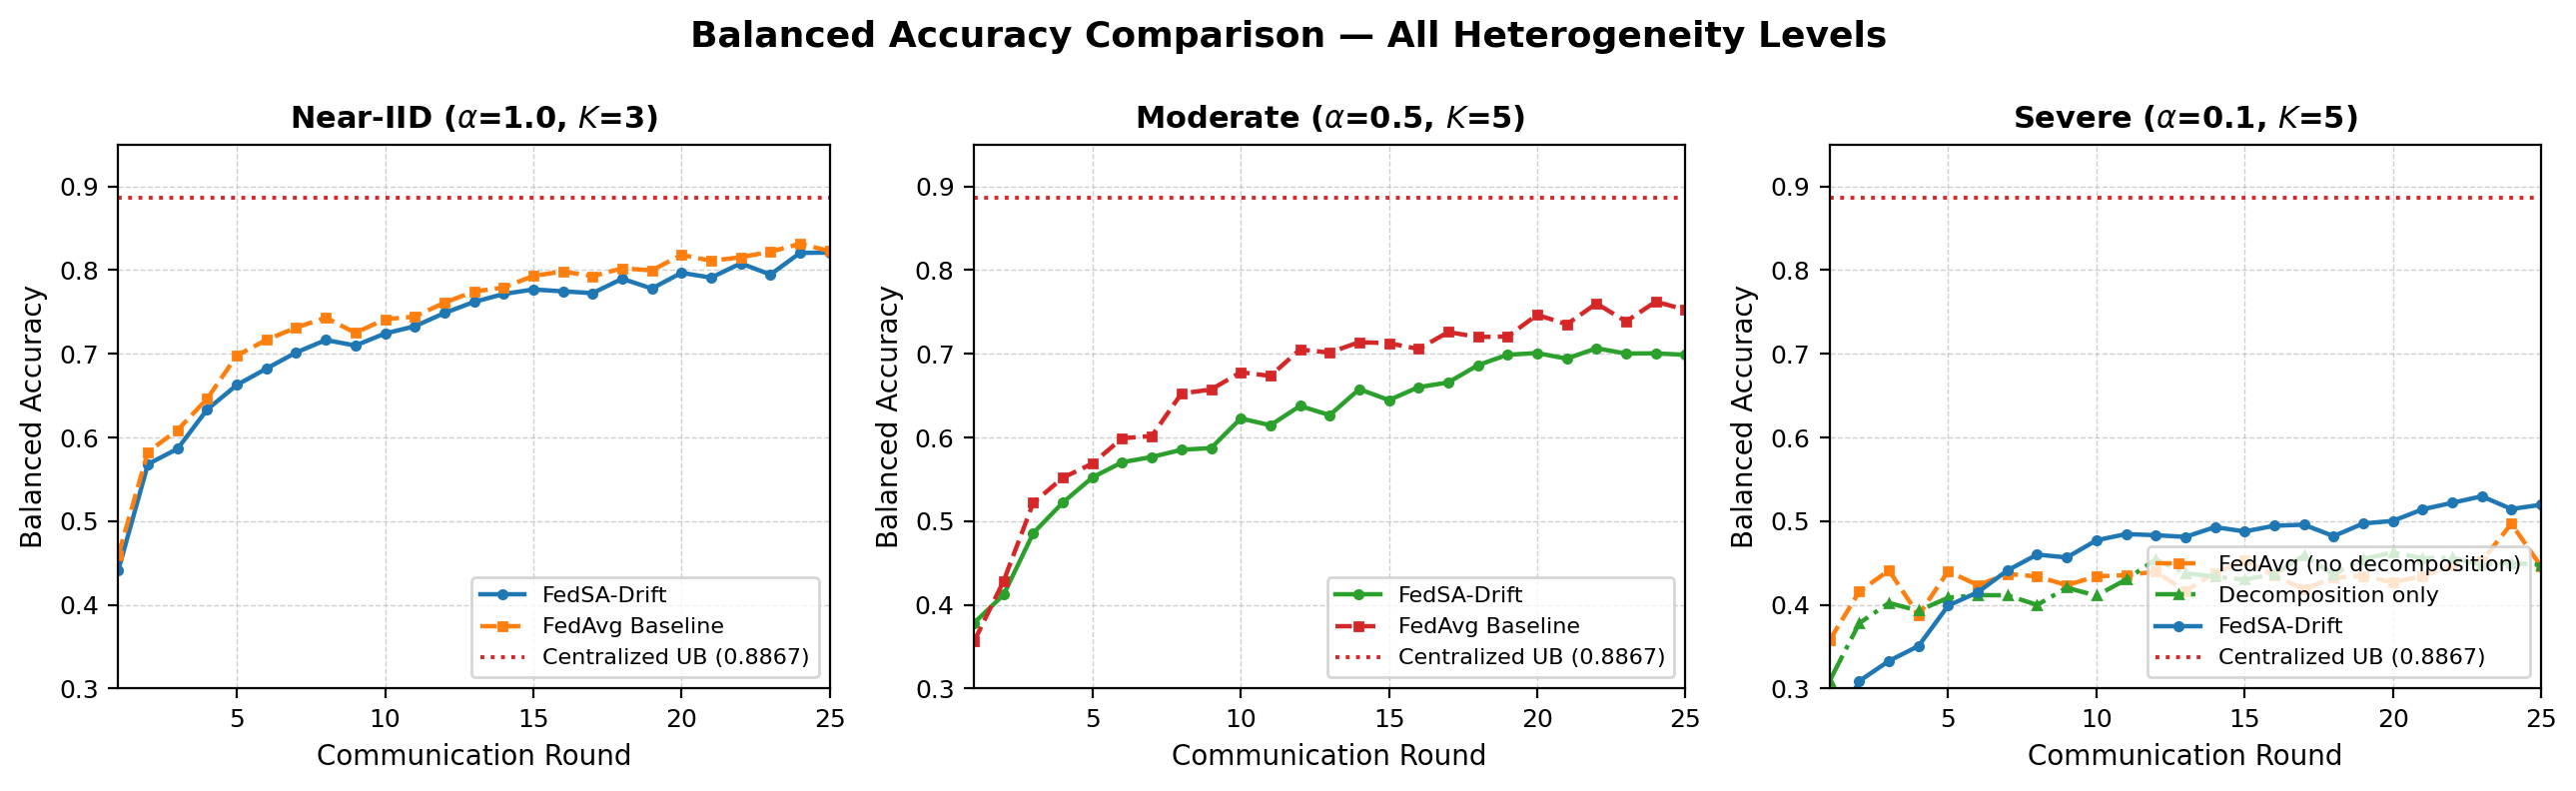
\includegraphics[width=\textwidth]{images/comparison_balanced_acc_all.png}
\caption{Balanced accuracy across all three heterogeneity levels: near-IID ($\alpha{=}1.0$, $K{=}3$), moderate ($\alpha{=}0.5$, $K{=}5$) and severe ($\alpha{=}0.1$, $K{=}5$). The severe panel additionally shows the no-decomposition baseline. The centralized upper bound is shown for reference. At $\alpha{=}0.1$ the no-decomposition baseline sits below \sadrift{} on this validation curve (0.4460 against 0.5196 at round 25), yet on the test split their mean per-client balanced accuracies are within one point (0.3778 against 0.3681) while the baseline records zero melanoma recall throughout. Balanced accuracy alone therefore does not distinguish the two.}
\label{fig:comparison_bal_acc}
\end{figure*}

Thus, global accuracy alone is insufficient for evaluating federated medical models. \sadrift{} offers a practical path toward stable and fair multi-institutional deployment.


\section{Reproducibility}
\label{sec:repro}

All code, including the model definition, the partitioning procedure, the aggregation rules, every ablation arm and the evaluation scripts, is publicly available at \url{https://github.com/apurbaaaa/layer-wised-personalised}. Every reported configuration is reproducible from a single command; the exact invocations are in \texttt{run\_reviewer\_matrix.sh} and \texttt{run\_tf\_alpha01.sh}.

Randomness is controlled by one seed, exposed as \texttt{--seed} and recorded in every run log, which governs both the model initialisation and the Dirichlet draw. All results in this paper use seed 42. The validation split is regenerated deterministically by \texttt{StratifiedShuffleSplit(test\_size=0.15, random\_state=42)} over the ground-truth CSV in its published row order, so the exact train and validation indices---and hence the per-client shards---are recoverable without transferring index files. The per-client class counts printed at the start of each run (reproduced in Figures~\ref{fig:severe_fedavg_bundle}--\ref{fig:severe_sadrift_bundle}) allow a reader to confirm that a regenerated partition matches ours.

We note as a deficiency that a single seed was used throughout; this is discussed under Limitations.

\section{Limitations}

Several limitations of this work should be acknowledged explicitly.

\textbf{Experimental scale and two kinds of uncertainty.} All experiments use $K \in \{3, 5\}$ clients and $\alpha \in \{0.1, 0.5, 1.0\}$, with a single training run per configuration. Two distinct sources of uncertainty affect the reported figures, and we are able to quantify only one of them.

\emph{Evaluation-set sampling} uncertainty---how far a number could move under a different test sample---is quantified directly. Per-class recall is a binomial proportion, so Wilson score intervals apply without repeated training; these are reported in Section~\ref{sec:intervals} and are tight enough for the melanoma ladder to have mutually disjoint intervals. Where a claim depends on a fixed trained model evaluated on held-out data, it therefore carries an interval estimate.

\emph{Training-run} uncertainty---seed-to-seed variability arising from a different Dirichlet partition draw and initialisation---is \emph{not} quantified, because it requires repeating each configuration across multiple seeds and each run costs approximately 10 GPU-hours. Figures such as the 58\% variance reduction and the +13.71 pp worst-client improvement remain single-trial point estimates in this respect, and we make no claim of statistical significance for them. Seeding is now an explicit and logged experimental parameter, so the reported runs are exactly reproducible, and we additionally verify that the $\alpha = 0.1$ effects are stable across the final five communication rounds rather than resting on a single round; but neither substitutes for a multi-seed study, which remains necessary future work. Validation at larger client counts ($K \ge 10$) likewise remains future work.

\textbf{What the shared global model contains.} Group~C comprises the metadata MLP and the fusion head; as the backbone is instantiated with no classifier of its own, the fusion head \emph{is} the classifier. Group~C is never aggregated, so the classifier carried by the shared global model remains at its initialisation for the whole run---we verified that all Group~C tensors are bit-identical to their initialisation after training, while Group~A tensors have changed.

This does not make the shared model a random classifier, and its accuracy is not degenerate. Every client begins local training from that same initial head, and gradients reach the backbone through it, so the aggregated backbone is optimised to produce features that are discriminative \emph{under that particular fixed projection}. The composite is a functioning model: at $\alpha{=}0.1$ it reaches 0.5196 balanced accuracy, which is in fact \emph{higher} than the 0.4382 mean achieved by the personalized client models on the same split. The shared model and the personalized models are different objects---one uses the common initial head, the others their own adapted heads---and neither dominates the other.

Two consequences follow. Global-model accuracy is meaningful \emph{within} the decomposed family, where every arm shares this construction. It is not directly comparable with a method that also aggregates its classifier, such as the no-decomposition baseline, whose shared model is a fully aggregated network. For cross-arm comparison we therefore use mean per-client accuracy, evaluating each client with the head it would actually deploy.

\textbf{Dispersion depends on the accuracy measure.} Our reported variance-reduction figures use the standard deviation of overall per-client accuracy. Under severe heterogeneity ($\alpha = 0.1$) the ordering reverses if balanced accuracy is used instead (0.0855 for \sadrift{} versus 0.0587 without drift weighting). This does not indicate degradation at any client: every client's balanced accuracy improves under drift-aware aggregation, but by an amount that scales with how many classes that client actually holds---clients observing seven or eight of the eight classes gain approximately 9~pp, whereas a client observing four gains 3~pp. Balanced accuracy is bounded by classes a client has never seen, so the benefit is unevenly distributed and dispersion in that measure widens even as every client improves.

\textbf{Ablation scope.} The three-way ablation of Section~\ref{sec:threeway} separates both components, but only at $\alpha = 0.1$ and with a single seed. At $\alpha \in \{0.5, 1.0\}$ only the drift component is isolated, because the corresponding no-decomposition configurations were not run and the earlier decomposed runs did not retain per-client checkpoints from which mean per-client accuracy could be reconstructed. Whether the division of labour we observe---decomposition supplying class coverage, drift weighting supplying utility and fairness---persists at milder heterogeneity is therefore untested. We would expect the effect to shrink as $\alpha$ increases, since class abandonment under FedAvg is itself a consequence of severe label skew.

\textbf{Aggregate accuracy at severe heterogeneity.} We do not claim that \sadrift{} improves overall or balanced accuracy at $\alpha = 0.1$. Standard FedAvg attains higher mean per-client accuracy (0.4702 versus 0.4264) and marginally higher balanced accuracy (0.3778 versus 0.3681) on the held-out test split. The case for \sadrift{} in this regime rests on class coverage, worst-client performance and inter-client dispersion, not on aggregate accuracy.

\textbf{Same-lesion contamination in the validation split.} The ISIC 2019 archive contains multiple photographs of the same lesion, and the metadata assigns a \texttt{lesion\_id} to 23,247 of the 25,331 images, covering 11,847 distinct lesions. Our validation split is a stratified random split over images, not over lesions. Auditing it, 1,881 lesions have images on both sides, so 2,340 of the 3,800 validation images (61.6\%) depict a lesion that also appears in the training partition. No image occurs in both splits, but sibling images of the same lesion do.

Validation-split figures are therefore optimistically biased, and this includes the centralized 0.8867 and every round-by-round result at $\alpha \in \{1.0, 0.5\}$. The magnitude is visible in the gap to the held-out test collection, where balanced accuracy falls to 0.368--0.378. We report this rather than leave it implicit because it bounds how the validation numbers should be read.

Two things are unaffected. Comparisons \emph{between} configurations remain valid, because every arm is trained and evaluated on the identical split, so the contamination is common to all of them and cancels in the differences that carry our claims---worst-client accuracy, dispersion and the component ablation. And all test-split results, including the entire three-way ablation of Section~\ref{sec:threeway} and the melanoma finding, are computed on the separate ISIC 2019 test collection and are not affected. A lesion-grouped split would give unbiased absolute validation figures and is the correct design for future work; it requires retraining every configuration and was not possible within the compute available for this revision.

\textbf{Baseline set.} Our comparisons are to FedAvg, to the decomposition without drift weighting, and to a variant with the decomposition removed. We did not evaluate against FedProx, SCAFFOLD, FedBN, FedRep, FedPer, FedBABU, FedNova or FedDyn. This is the most consequential gap in the evaluation: the three-way ablation of Section~\ref{sec:threeway} establishes what each of \emph{our} components contributes, but it cannot establish that this design is preferable to an established personalized method. In particular, a substantial part of our benefit may come simply from not sharing the classification head, which FedPer, FedRep and FedBABU also do. We state in Section~\ref{sec:positioning} that we make no superiority claim over that literature, and a controlled comparison against at least FedProx, FedBN and FedRep is the first priority for further work.

\textbf{Client scale.} All experiments use $K \in \{3,5\}$. Deployments of interest involve tens to hundreds of institutions, and several properties of the method are scale-sensitive in ways we have not measured: the inverse-distance weights are normalised over $K$, so the concentration bound of Section~\ref{sec:weight_analysis} tightens as $K$ grows, and partial client participation---which we do not use, as $\texttt{client\_frac}{=}1.0$ throughout---would make the drift estimate noisier. Results at $K \in \{10,20,50\}$ are needed before any claim about deployment scale.

\textbf{Aggregation design choices are unvalidated.} The decomposition boundary (stages 0--1 versus 2--3), the Euclidean distance, and the inverse-distance functional form were fixed a priori and not compared against alternatives such as different split points, cosine similarity, or softmax, exponential and inverse-square weightings. Section~\ref{sec:weight_analysis} gives our reasoning for each, but reasoning is not evidence, and we cannot claim these choices are optimal.

\textbf{Client count and heterogeneity are confounded.} The three federated configurations are $(\alpha{=}1.0, K{=}3)$, $(\alpha{=}0.5, K{=}5)$ and $(\alpha{=}0.1, K{=}5)$. They do not form a factorial grid: any comparison between the near-IID setting and the other two changes both the concentration parameter and the number of clients simultaneously, so the two effects cannot be separated there. The $\alpha{=}0.5$ versus $\alpha{=}0.1$ comparison, and the three-way ablation of Section~\ref{sec:threeway}, both hold $K$ fixed at 5 and are unaffected.

\textbf{No calibration or uncertainty analysis.} We report discrimination metrics only. For a triage setting the operating threshold, the calibration of predicted probabilities, and some expression of predictive uncertainty matter at least as much as recall at the default threshold, and a model that abandons a class silently is precisely the case where an uncertainty estimate would be informative. We report neither reliability diagrams nor expected calibration error, and all per-class figures are taken at the $\arg\max$ decision rule. This is a substantive gap for clinical deployment and not merely a presentational one.

\textbf{Single dataset.} All federated experiments use ISIC 2019. Generalization to other dermatology datasets or to different medical imaging modalities is not verified and remains an open question.

\textbf{Simulation environment.} All federated experiments are simulated rather than deployed: clients are trained sequentially within one process on NVIDIA A40 hardware (the $\alpha{=}0.1$ configurations were run concurrently across three such GPUs, one arm per device, which affects wall-clock time but not results). Real-world deployment involves network latency, heterogeneous edge hardware, and bandwidth constraints not captured in this simulation.

\textbf{Baseline conditions.} The published baselines in Table~\ref{tab:sota_comparison} are evaluated under different experimental conditions. A fully controlled re-implementation of FedMHA, FedAPM, and EFTViT on ISIC 2019 under identical conditions was not performed; the comparison is therefore contextual rather than definitive.

\section{Conclusion and Future Work}

This paper has proposed a structure-aware federated learning framework called \sadrift{} for multimodal skin lesion classification. The framework was developed to specifically target stability and fairness issues that arise from heterogeneous clinical data distributions. The architecture of \sadrift{} decomposes model parameters into early vision backbone layers, deep semantic Transformer layers and client-specific multimodal heads, thus allowing for both selective aggregation and individual personalization of the aggregated model within the Vision Transformer framework. To stabilize the deep semantic representations at the server, this paper implements a drift-aware inverse-distance aggregation mechanism during the aggregation process. This mechanism does not alter the local optimization objectives or add additional hyperparameters for regularisation. The clearest evidence for the framework comes from the held-out ISIC 2019 test collection under severe heterogeneity, where the choice of aggregation scheme determines whether a diagnostic class survives training at all. Experimental results further show that \sadrift{} achieves comparable aggregate accuracy while substantially improving robustness at the client level. Under moderately heterogeneous conditions ($\alpha = 0.5$, $K = 5$), the drift-aware aggregation mechanism reduced inter-client performance variability by approximately 39\% in a single experimental trial, with minimal computational overhead.

Under severe heterogeneity ($\alpha = 0.1$, $K = 5$) a three-way ablation on a held-out test split separates the two mechanisms. Standard FedAvg achieves the highest aggregate accuracy but abandons four of eight diagnostic classes outright, recording zero melanoma recall for every client---including the institution that holds almost all of the melanoma cases---because size-weighted aggregation is dominated by a client holding none. The parameter decomposition restores all eight classes at a cost in mean accuracy, and drift-aware weighting then recovers most of that cost while raising the worst-client floor by 21.5 points and reducing dispersion by 67\%. That the two configurations differ by only one point of balanced accuracy despite these very different clinical profiles is itself instructive: aggregate metrics, balanced accuracy included, cannot detect the complete loss of a diagnostic category. Future work will examine how \sadrift{} generalizes across datasets beyond ISIC 2019, particularly in settings where class distributions and imaging protocols differ substantially between institutions. The broader implication is that federated frameworks designed for medical imaging should be evaluated against client-level variance from the outset, not retrofitted for fairness after the fact. As a result, it can be concluded that using only global metrics to evaluate the performance of federated models for medical imaging is insufficient, and that stability and fairness must also be considered as essential criteria for the clinical deployment of federated models.

Future research may focus on investigating the use of adaptive layer-wise drift sensitivity for increased control over how aggregation occurs within each layer of a Transformer architecture. In addition, parameter-efficient methods of personalizing large models, such as adapter-based or low-rank adaptation schemes, could reconcile the sharing of global knowledge from the model with institution-specific specialization. There is also an opportunity to improve worst-case performance guarantees by incorporating fairness-based optimization criteria and methods at the server level. In addition, using structured quantization to achieve communication efficiency could potentially allow the implementation of a large model across many resource-constrained edge devices. Cross-dataset generalization and domain shift remain open questions for assessing the clinical robustness of the model. Finally, integrating drift-based aggregation schemes with formal privacy techniques such as secure aggregation and differential privacy could provide additional theoretical support for the use of federated Vision Transformer models in medical imaging applications.




\begin{thebibliography}{99}

\bibitem{Arnold2022}
M. Arnold, M. Singh, S. Laversanne, D. Vignat, J. Ferlay, and I. Soerjomataram,
“Global burden of cutaneous melanoma in 2020 and projections to 2040,”
\emph{JAMA Dermatology}, vol. 158, no. 5, pp. 495–503, 2022.

\bibitem{Hay2014}
R. J. Hay, N. E. Johns, H. C. Williams, et al.,
“The global burden of skin disease in 2010: An analysis of the prevalence and impact of skin conditions,”
\emph{Journal of Investigative Dermatology}, vol. 134, no. 6, pp. 1527–1534, 2014.

\bibitem{Aguirre2024}
J. Aguirre, et al.,
“A comparative analysis of CNN models and vision transformers for skin lesion classification,”
\emph{SOL-SBC (Sociedade Brasileira de Computação)}, 2024.

\bibitem{Voigt2017}
P. Voigt and A. Von dem Bussche,
\emph{The EU General Data Protection Regulation (GDPR): A Practical Guide}.
Cham, Switzerland: Springer, 2017.

\bibitem{Law2023}
S. Law,
“Consumer data privacy: EU’s GDPR vs. China’s PIPL,”
\emph{Bloomberg Law}, 2023.

\bibitem{McMahan2017}
B. McMahan, E. Moore, D. Ramage, S. Hampson, and B. A. y Arcas,
“Communication-efficient learning of deep networks from decentralized data,”
in \emph{Proc. 20th Int. Conf. Artificial Intelligence and Statistics (AISTATS)}, 2017, pp. 1273–1282.

\bibitem{Rieke2020}
N. Rieke, J. Hancox, W. Li, et al.,
“The future of digital health with federated learning,”
\emph{NPJ Digital Medicine}, vol. 3, no. 119, 2020.

\bibitem{Zhao2018}
Y. Zhao, M. Li, L. Lai, N. Suda, D. Civin, and V. Chandra,
“Federated learning with non-iid data,”
arXiv:1806.00582, 2018.

\bibitem{Li2020}
T. Li, A. K. Sahu, M. Zaheer, M. Sanjabi, A. Talwalkar, and V. Smith,
“Federated optimization in heterogeneous networks,”
in \emph{Proc. MLSys}, 2020.

\bibitem{Nunnari2020}
F. Nunnari, G. Pappalardo, and C. Lombardo,
“A study on the fusion of pixels and patient metadata in CNN-based classification of skin lesion images,”
in \emph{Proc. IJCNN}, 2020.

\bibitem{Gessert2020}
N. Gessert, M. Nielsen, M. Shaikh, R. Werner, and A. Schlaefer,
“Skin lesion classification using ensembles of multi-resolution EfficientNets with meta data,”
in \emph{ISIC 2019 Challenge Proceedings}, 2020.

\bibitem{Zhu2025}
X. Zhu, et al.,
“FedAPM: Federated learning via ADMM with partial model personalization,”
in \emph{Proceedings of the 31st ACM SIGKDD Conference on Knowledge Discovery and Data Mining (KDD ’25)}, 2025.

\bibitem{Karimireddy2020}
S. P. Karimireddy, S. Kale, M. Mohri, S. Reddi, S. Stich, and A. T. Suresh,
“SCAFFOLD: Stochastic controlled averaging for federated learning,”
in \emph{Proc. ICML}, 2020.

\bibitem{Collins2021}
L. Collins, H. Hassani, A. Mokhtari, and S. Shakkottai,
“Exploiting shared representations for personalized federated learning,”
in \emph{Proc. ICML}, 2021.

\bibitem{Darzi2024}
A. Darzi, et al.,
“Tackling heterogeneity in medical federated learning via aligning vision transformers,”
arXiv preprint, 2024.

\bibitem{Li2021}
T. Li, S. Hu, A. Beirami, and V. Smith,
“Ditto: Fair and robust federated learning through personalization,”
in \emph{Proc. ICML}, 2021.

\bibitem{Zhao2025}
Y. Zhao, H. Chen, L. Wang, and J. Liu,
“Federated Vision Transformer with adaptive focal loss for medical image classification,”
arXiv preprint, 2025.

\bibitem{Wu2024}
J. Wu, X. Li, Y. Zhang, and K. Huang,
“EFTViT: Efficient federated training of vision transformers with masked images on resource-constrained clients,”
arXiv preprint, 2024.

\bibitem{Naeem2025}
M. Naeem, et al.,
“Automated skin cancer detection using MedFusionNet with attention-based fusion of ConvNeXt and vision transformer,”
\emph{Scientific Reports}, 2025.

\bibitem{Alshdaifat2025}
E. Alshdaifat, et al.,
“Triple-Stream Transformer architecture for multi-class skin cancer classification in dermoscopic images,”
\emph{Journal of Posthumanism}, 2025.

\bibitem{HyperFusionNet2025}
Y. Li, et al.,
“HyperFusionNet: Vision transformer-based early melanoma detection with precise lesion segmentation,”
\emph{Scientific Reports}, 2025.

\bibitem{HasanRifat2024}
M. Hasan and S. Rifat,
“Hybrid ensemble of segmentation-assisted classification and gradient-boosted decision trees for skin cancer detection,”
arXiv preprint, 2024.

\bibitem{Zoravar2024}
S. Zoravar, et al.,
“Domain adaptive skin lesion classification via conformal ensemble of vision transformers,”
arXiv preprint, 2024.

\bibitem{Wegley2026}
A. Wegley, et al.,
“Dermatology skin lesion image analysis,”
\emph{Scholars' Mine Research Repository}, 2026.

\bibitem{SkinDiversity2024}
M. Alipour, et al.,
“Skin type diversity in skin lesion datasets: A review,”
\emph{Current Dermatology Reports}, 2024.

\bibitem{Guan2024}
Q. Guan, et al.,
“Federated learning for medical image analysis: A survey,”
\emph{Pattern Recognition}, 2024.

\bibitem{Subramanian2025}
S. Subramanian, et al.,
“Skin cancer classification and detection using federated learning,”
in \emph{Proc. 3rd Int. Conf. Futuristic Technology (INCOFT)}, 2025.

\bibitem{Yaqoob2023}
T. Yaqoob, et al.,
“Federated machine learning for skin lesion diagnosis: An asynchronous and weighted approach,”
\emph{Diagnostics}, 2023.

\bibitem{Paxton2024}
R. Paxton, et al.,
“Skewness-guided pruning of multimodal Swin transformers for federated skin lesion classification on edge devices,”
arXiv preprint, 2024.

\bibitem{Zuo2024}
Q. Zuo, et al.,
“FedViT: Federated continual learning of vision transformer at edge,”
\emph{Future Generation Computer Systems}, 2024.

\bibitem{Yao2024}
L. Yao, et al.,
“Task-agnostic federated learning with imbalanced data,”
arXiv preprint, 2024.

\bibitem{Almalik2022}
H. Almalik, et al.,
“Self-ensembling vision transformer (SEViT) for robust medical image classification,”
in \emph{Proc. MICCAI}, 2022.

\bibitem{Imam2023}
M. Imam, et al.,
“On enhancing the robustness of vision transformers: Defensive diffusion,”
arXiv preprint, 2023.

\bibitem{Narimani2024}
M. Narimani, et al.,
“FedRP: A communication-efficient approach for differentially private federated learning using random projection,”
arXiv preprint, 2024.

\bibitem{Mohri2019}
M. Mohri, G. Sivek, and A. T. Suresh,
“Agnostic federated learning,”
in \emph{Proc. 36th Int. Conf. Machine Learning (ICML)}, 2019, pp. 4615--4625.

\end{thebibliography}

\begin{IEEEbiography}[{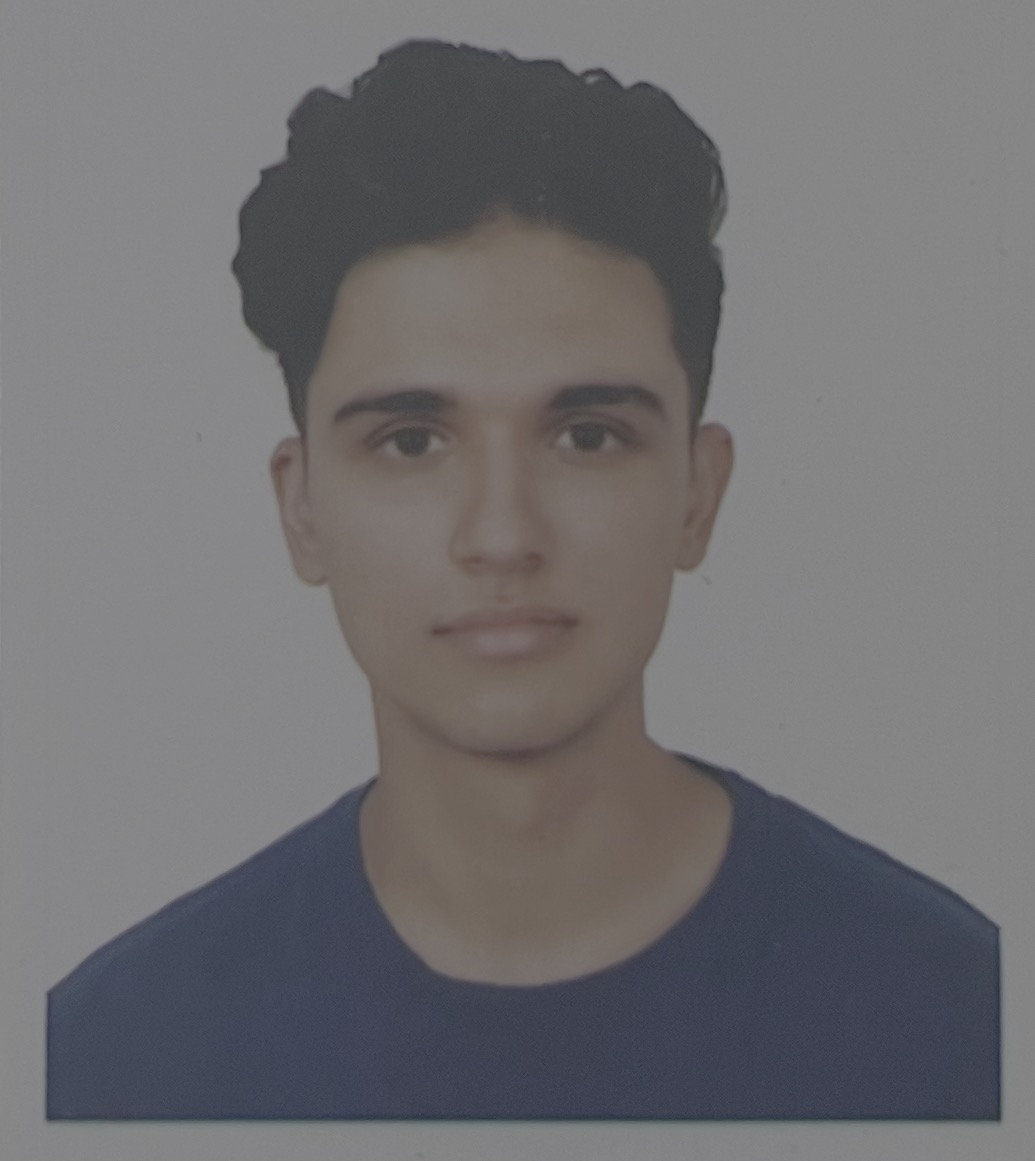
\includegraphics[width=1in,height=1.25in,clip,keepaspectratio]{images/Apurba.jpg} }]{APURBA KOIRALA}
received his secondary education from Rato Bangala School, Kathmandu, Nepal. He is currently pursuing a Bachelor of Technology degree in Computer Science and Engineering at Vellore Institute of Technology, Vellore, India. His research interests include machine learning, deep learning, federated learning, and the application of artificial intelligence in healthcare and neuroimaging. He intends to conduct further research at the nexus of AI and biomedical sciences, having worked on several projects centred on medical data analysis and privacy-preserving AI.

\end{IEEEbiography}

\begin{IEEEbiography}[{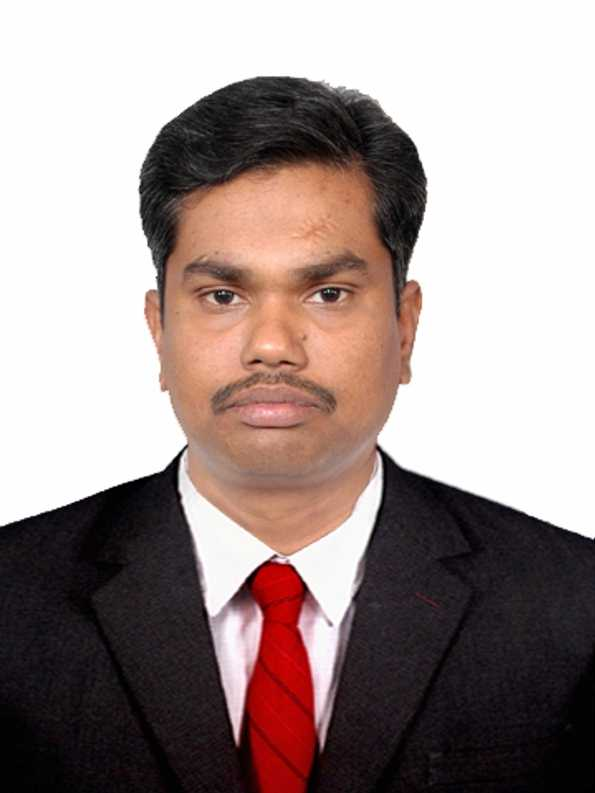
\includegraphics[width=1in,height=1.25in,clip,keepaspectratio]{images/rkannanimage.png}}]{RAJESHKANNAN REGUNATHAN}
received his M.Tech.\ degree in Computer Science and Engineering from SASTRA University, Tanjore, India, and his Ph.D.\ degree in Computer Science and Engineering from Vellore Institute of Technology, Vellore, India. He is currently a Professor at VIT, Vellore, India. His areas of interest include cloud computing, artificial intelligence, natural language processing, and data science. He has over 20 years of teaching experience and has published numerous papers in international journals and conferences. He is a member of CSI and IEEE (WIE).

\end{IEEEbiography}

\begin{IEEEbiography}[{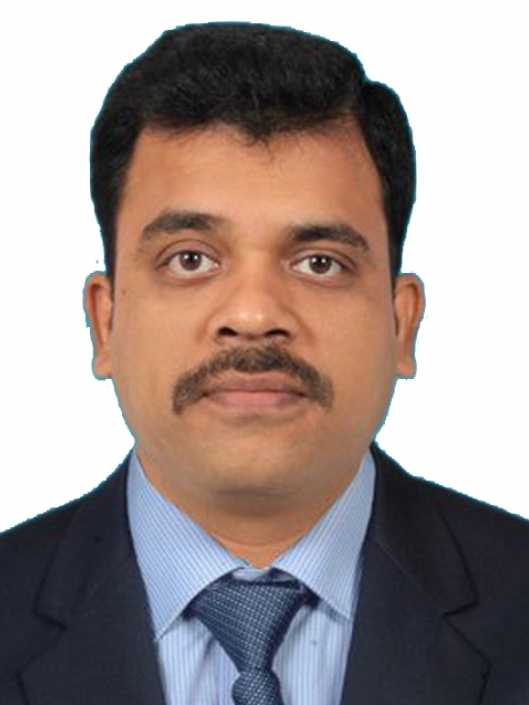
\includegraphics[width=1in,height=1.25in,clip,keepaspectratio]{images/raksaravanaguruimage.png}}]{RA K SARAVANAGURU}
is a Professor in the Department of Information Security, School of Computer Science and Engineering, Vellore Institute of Technology (VIT), Vellore, India, where he has been serving since 2004. He has over 25 years of teaching, research, and academic administration experience, and previously served as Assistant Dean (Academics). His research interests include Artificial Intelligence, Generative AI, Context-Aware Computing, Blockchain Technology, Deep Learning, and Software Design Patterns. He has published numerous research articles in reputed international journals and conferences, with notable contributions in areas such as Internet of Vehicles, Digital Evidence Management, Healthcare Analytics, and Intelligent Computing Systems.

\end{IEEEbiography}

\EOD

\end{document}
